\documentclass[12pt]{report}
\usepackage{jrl_thesis}
\usepackage{fancyheadings}
\usepackage{natbib}
\usepackage{setspace}               % this package defines the spacing of your thesis and should be included
\usepackage{amsmath}
\usepackage{amsfonts}
\usepackage{amssymb}
\usepackage{amsthm}
\usepackage{mathtools}
\usepackage{url}
%\usepackage{cite}
%\usepackage{epsfig}
\usepackage{xspace}
\usepackage{graphicx}
%\usepackage{subfigure}
\usepackage{color, colortbl}
\usepackage{listings}
\usepackage{stmaryrd}
 %\usepackage{algorithm}
%\usepackage{algorithmic}

\usepackage[boxed, vlined, linesnumbered]{algorithm2e}

%\usepackage[noline,boxed]{algorithm2e}
%\usepackage[skins]{tcolorbox}

\setcounter{secnumdepth}{4}
\setcounter{tocdepth}{2}


\usepackage{algcompatible}
\usepackage{caption}
\usepackage[absolute]{textpos}
%\usepackage[inference]{semantic}
%\usepackage{multicol}
%\usepackage{wrapfig}
\usepackage{multirow}
\usepackage{todonotes}
\usepackage{tikz}
%\usepackage{mathtools}
%\usepackage{enumitem}

\usepackage{amsmath}
\usepackage{chngcntr}
\counterwithin{figure}{chapter}
\counterwithin{equation}{chapter}
\counterwithin{table}{chapter}
%\counterwithin{algorithm}{chapter}
%\counterwithin{theorem}{chapter}


\usepackage{algpseudocode}

\usepackage{wrapfig}
\usepackage{lipsum}
\usepackage{float}

\usepackage{enumerate}

\usepackage{comment}
\usepackage{color}
\specialcomment{notes}{\begingroup\sffamily\color{red}}{\endgroup}

\newcommand\red[1]{\color{red}#1}
\newcommand{\rewrite}{\mathtt{REWRITE}}


\usetikzlibrary{matrix,positioning,mindmap,automata,fit,backgrounds,
shapes, arrows,petri,calc, decorations.pathreplacing}


\newif\ifspace\spacefalse
\graphicspath{{figs/}}
\usepackage{subcaption}

\newcommand\tuple[1]{\langle #1 \rangle}

% \pagestyle{plain}
% \pagenumbering{arabic}

%\theoremstyle{plain}
%\newtheorem{observation}[theorem]{Observation}

%\setlength{\textwidth}{12.9cm}
%\setlength{\parskip}{0.001mm}

\newcommand{\SK}[1]{\textbf{#1}\footnote{Check here}}
\newcommand{\knowsnonce}[1]{has(#1)}

\newcommand{\ra}[1]{((\neg a_{#1} \, \U \, r_{#1}) \, \U \, a_{#1})}
\newcommand{\wrt}{\mathit{write}}

\newcommand{\rcvd}[4]{\mathit{rcvd}_#1(#2.#3.#4)}
\newcommand{\sendmsg}[5]{\send(#1_p.#2_p.#3.#4.#5)}
\newcommand{\sendm}[3]{\send({#1.#2.#3})}
\newcommand{\sentm}[4]{ {sent_{{#1}}(#2.#3.#4) } }
\newcommand{\sentmsg}[6]{ sent_{#1}(#2_p.#3_p.#4_l.#5_l.#6)}
\newcommand{\rcvdm}[4]{ {\rcvd_{{#1}}(#2.#3.#4) } }
\newcommand{\rcvdmsg}[6]{ rcvd_{#1}(#2_p.#3_p.#4_l.#5_l.#6)}
\newcommand{\fresh}[2]{\mathit{fresh}_{#1}(#2)}
\newcommand{\has}[2]{has_{#1}(#2)}
\newcommand{\PK}{\mathit{PK}}
\newcommand{\new}{\mathit{new}}
\newcommand{\ns}{\mathit{ns}}
\newcommand{\ps}{\sample}
\newcommand{\LC}{\mathit{LC}}


\newcommand{\I}[1]{\mathit{#1}}
\newcommand{\syntru}{\I{true}} %syntactical true
\newcommand{\synfals}{\I{false}} %syntactical false
\newcommand{\inftrace}{\sigma}
\newcommand{\fintrace}{\alpha}
\newcommand{\FinTrace}{A}
\newcommand{\tru}{\mathsf{true}}
\newcommand{\fals}{\mathsf{false}}
\newcommand{\word}{w}
\newcommand{\emptyword}{\epsilon}
\newcommand{\alphabet}{\Sigma}
\newcommand{\LS}{\mathit{Snap}}
\newcommand{\SM}{\mathit{SM}}
\newcommand{\TT}{{\top_p}}
\newcommand{\FT}{{\bot_p}}
\newcommand{\LTL}{{\sc Ltl}\xspace}
\newcommand{\LTLtri}{{\sc Ltl}\textsubscript{3}\xspace}
\newcommand{\LTLk}{$\mbox{\sc Ltl}_{2k+4}$\xspace}
\newcommand{\RVLTL}{{\sc Rv-Ltl}\xspace}
\newcommand{\FLTL}{{\sc Fltl}\xspace}
\newcommand{\LTLfour}{{\sc Ltl}\textsubscript{4}\xspace}
\newcommand{\zplus}{\mathbb{Z}_{\geq 0}}
\newcommand{\prog}{\mathcal{D}}
\newcommand{\AP}{\mathit{AP}}
\newcommand{\ap}{\mathit{ap}}
\newcommand{\F}{\mathbf{F}}
\newcommand{\G}{\mathbf{G}}
\newcommand{\X}{\mathbf{X}}
\newcommand{\U}{\mathbf{U}}
\newcommand{\udef}{\natural}
\newcommand{\monitor}{\mathcal{M}}
\newcommand{\sample}{\mathcal{S}}
\newcommand{\trace}{\sigma}
\newcommand{\alltrace}{\mathrm{\Xi}}
%\newcommand{\pred}{\mathcal{F}}
\newcommand{\pred}{\mathbf{project}}
\newcommand{\extr}{\mathbf{x}}
\newcommand{\state}{s}

\newcommand{\AN}{\mathit{AN}}
%\newcommand{\so}{\mathit{sa}}
\newcommand{\io}{\mathit{ia}}
\newcommand{\wo}{\mathit{wa}}
\newcommand{\gstate}{\mathcal{S}}
\newcommand{\trans}{\mathcal{T}}
\newcommand{\srs}{\mathfrak{s}}
\newcommand{\exprop}{\neg \mathit{spawn} \; \U \; \mathit{init}}

\newcommand{\BB}[1]{$\clubsuit$\footnote{$\clubsuit$ BB: #1}}
\newcommand{\SR}[1]{$\clubsuit$\footnote{$\clubsuit$ SR: #1}}
\newcommand{\DR}[1]{$\clubsuit$\footnote{$\clubsuit$ DR: #1}}

\newcommand{\algorithmicinput}{\textbf{Input:}}
\newcommand{\INPUT}{\item[\algorithmicinput]}
\newcommand{\algorithmicoutput}{\textbf{Output:}}
\newcommand{\OUTPUT}{\item[\algorithmicoutput]}
\renewcommand{\topfraction}{0.96}
\renewcommand{\bottomfraction}{0.95}
\renewcommand{\textfraction}{0.01}
\renewcommand{\floatpagefraction}{1}
\renewcommand{\dbltopfraction}{.97}
\renewcommand{\dblfloatpagefraction}{.99}

\newcommand\code[1]{\textsf{\small #1}}

% comments
\newcommand{\remove}[1]{}
\newcommand{\borzoo}[1]{\marginpar{\small \emph{borzoo:} #1}}
\newcommand{\sergio}[1]{\marginpar{\textcolor{blue}{\small \emph{sergio:} #1}}}
\newcommand{\pierre}[1]{\marginpar{\textcolor{red}{\small \emph{pierre:} #1}}}
\newcommand{\david}[1]{\marginpar{\small \emph{david:} #1}}




% for the appendix
%\newenvironment{theorem-repeat}[1]{\begin{trivlist}
%\item[\hspace{\labelsep}{\bf\noindent Theorem~\ref{#1} }]}%
%{\end{trivlist}}

%abbrviations for topology
\newcommand{\sfont}[1]{$\mathsf{#1}$}
\newcommand{\m}[1]{\ensuremath{\mathcal{#1}}\xspace}
\newcommand{\yes}{\mbox{\rm ``yes''}} 
\newcommand{\no}{\mbox{\rm ``no''}}
\newcommand{\ID}{\mbox{\rm ID}}
\newcommand{\sign}{\mbox{\sl sign}}
\newcommand{\val}{\mbox{\sl val}}
\newcommand{\mval}{\mbox{\sl mval}}
\newcommand{\setofval}{\mbox{\sl set}}
\renewcommand{\deg}{\mbox{\sl deg}}
\newcommand{\set}{\mbox{\sl set}}
\renewcommand{\dim}{\mbox{\sl dim}}
\newcommand{\carrier}{\mbox{\sl carrier}}
\newcommand{\opin}{\mbox{\rm \#opinion}}
\newcommand{\altn}{\mbox{\rm \#altern}}
\newcommand{\nan}{\mbox{\rm negalt}}
\newcommand{\complex}{\mbox{\sl complex}}
\newcommand{\an}{\alpha}
%\newcommand{\nan}{\bar{\alpha}}
\newcommand{\od}{orientation-detection}
\newcommand{\Od}{Orientation-detection}
\newcommand{\skel}{\mbox{\rm skel}}
\renewcommand{\tilde}[1]{\widetilde{#1}}
\newcommand{\ext}[1]{\ensuremath{\tilde{\mathcal{#1}}\xspace}}
\newcommand{\bd}{\partial}
\newcommand{\ffloor}[2]{\lfloor\frac{#1}{#2}\rfloor}
\newcommand{\floor}[1]{\left\lfloor#1\right\rfloor}
\newcommand{\INTLV}{\mathcal{I}}

\newcommand{\Exltl}{Extended \LTLtri monitor}
\newcommand{\DSM}{decentralized synchronous monitoring}
\newcommand{\intersection}{\mathcal{I}^\monstate}
\newcommand{\verdict}{V}
\newcommand{\valuation}{\nu}
\newcommand{\pevent}{E}
\newcommand{\events}{states}
\newcommand{\event}{state}
\newcommand{\monstate}{q}
\newcommand{\correctverd}{\monstate_c}
\newcommand{\correctverdict}{correct verdict}
\newcommand{\truthvalue}{truth value}
\newcommand{\abstate}{LS}
\newcommand{\absfunc}{\mu}
\newcommand{\indisting}{indisting?}
\newcommand{\disting}{disting?}
\newcommand{\dep}{covered?}
\newcommand{\partition}{PARTITION}
\newcommand{\partitionn}{partition}
\newcommand{\splitt}{SPLIT}
\newcommand{\splt}{split}
%\newcommand{\snap}{Snap}
\newcommand{\snap}{\mathit{Snap}}
\newcommand{\indist}{indistinguishable}
\newcommand{\dist}{distinguishable}
\newcommand{\covered}{covered}
\newcommand{\localreg}{local snapshot}





\newtheorem{definition}{Definition}
\numberwithin{definition}{chapter}

\newtheorem{theorem}{Theorem}
\numberwithin{theorem}{chapter}

\newtheorem{lemma}{Lemma}
\numberwithin{lemma}{chapter}

\newtheorem{claim}{Claim}
\numberwithin{claim}{chapter}

\newtheorem{corollary}{Corollary}
\numberwithin{corollary}{chapter}

%\newcommand{axiom}{Axiom}



\title{Decentralized Crash-Resilient Runtime Verification}
\author{Shokoufeh Kazemlou}

\prevdegreeone{M.Sc.}

\prevdegreetwo{M.Sc.}

\submitdate{December 2017}

\copyrightyear{2017}

\principaladviser{Dr. Borzoo Bonakdarpour}
               % your information goes here

% add all other packages that you need to use here.

% ********************************
\begin{document}
\beforepreface                      % command to create the parts of your thesis that come before the preface like title and etc.

 % \include{dedic}
  \prefacesection{Abstract}



Runtime Verification is a technique to extract information from a running 
system in order to detect executions violating a given correctness 
specification. In this thesis, we study distributed synchronous/asynchronous 
runtime verification of systems. In our setting, there is a set of distributed 
monitors that have only partial views of a large system and are subject to 
failures. In this context, it is unavoidable that monitors may have different 
views of the underlying system, and therefore may have different valuations of 
the correctness property. In this thesis, we propose an automata-based 
synchronous monitoring algorithm that copes with $f$ crash failures in a 
distrbuted setting. The algorithm solves the synchronous monitoring problem in 
$f+1$ rounds of communication, and significantly reduces the message size 
overhead. We also propose an algorithm for distributed crash-resilient 
asynchronous monitoring that consistently monitors the system under inspection 
without any communication between monitors. Each local monitor emits a verdict 
set solely based on its own partial observation, and the intersection of the 
verdict sets will be the same as the verdict computed by a centralized monitor 
that has full view of the system.     












  \prefacesection{Acknowledgements}

Foremost, I would like to express my sincere gratitude to my supervisor Dr. Borzoo Bonakdarpour for the continuous support of my M.Sc. study and research, for his patience, motivation, and immense knowledge. I could not have imagined having a better mentor for my M.Sc. study.
I am very grateful to Professor Ryszard Janicki and Professor Mark Lawford for graciously agreeing to be my examiners and for their invaluable comments and suggestions. I am also grateful for the funding and support provided by the Natural Sciences and Engineering Research Council of Canada (NSERC).
Finally, I would like to thank my loved ones, who have supported me and encouraged me  throughout my years of study and through the process of researching and writing this thesis. 





 % \prefacesection{Notation and abbreviations}

Your notations go here.


\afterpreface                      % command to create the parts of your thesis that come after your preface like contents and etc.

  \chapter{Introduction}
\label{chap:introduction}

In a computing system, {\em correctness} refers to the assertion that a system
satisfies its specification. Software errors are an everyday problem. They 
occur for a variety of reasons like coding, hardware or network errors. There 
exist many techniques to ensure correctness in computing systems, most 
notably:

\begin{itemize}


\item Model checking is a fully automated push-button method to check 
that every execution path of the system under scrutiny satisfies its 
specification, usually given in some temporal logic formula.


\item Theorem proving as a semi-automated way to rigorously demonstrate that 
the system under inspection complies with its specification usually defined in 
higher-order logic.


 \item Testing is a way to detect such failures by checking for the presence of faults for a set of executions.
 

\end{itemize}

Recently, there has been an emerging interest on monitoring a software 
system to discover bugs in obscure corner cases that can only be observed 
during online execution. Runtime verification (RV) refers to a technique,  
where a monitor checks at run time whether or not the execution of a system 
under inspection satisfies a given correctness property. RV complements  
exhaustive verification methods such as model checking and theorem proving, as
well as incomplete solutions such as testing and debugging. Exhaustive 
verification often requires developing a rigorous abstract model of the 
system and suffers from the infamous {\em state-explosion problem}. Testing  
and debugging, on the other hand, provide us with under-approximated confidence 
about the correctness of a system as these methods only check for the presence 
of defects for a limited set of scenarios.

\section{Decentralized Runtime Verification}

Most existing RV methods employ a central monitor that collects the executions 
of all components and then checks the system's global behaviour in terms of a 
linear-time temporal logic (LTL) formula. The existing work on RV techniques 
where the monitor consists of a set of components, each having a partial view 
of the system, is limited to the following:

\begin{itemize}
 \item Lattice-theoretic centralized and decentralized online
predicate 
detection in distributed systems has been studied
in \cite{cgnm13,mg05}. 
However, this line of work does not address
monitoring properties with temporal 
requirements.
This shortcoming is addressed in \cite{og07} for a fragment of
temporal operators, but for offline monitoring and in~\cite{mb15} for 
distributed monitoring of LTL specifications.

\item In~\cite{svar04}, the authors design a method for monitoring safety
properties in distributed systems using the past-time linear
temporal logic 
(PLTL). This work, however, is not sound,
meaning that valuation of some 
predicates and properties
 may be overlooked. This is because monitors gain 
knowledge
about the state of the system by piggybacking on
the existing 
communication among processes. That is, if
processes rarely communicate, then 
monitors exchange
very little information and, hence, some violations of
properties may remain undetected.

\item Runtime verification of LTL for synchronous distributed
systems, where 
processes share a single global clock, has
been studied in~\cite{bf16,cf16}.

\end{itemize}

Another short coming of existing RV methods is that they assume a fault-free 
setting, where each individual monitor is resilient to failures. In fact, 
handling monitors subject to failures, creates significant challenges specially 
in asynchronous monitoring, as local monitors would not be able to agree on the 
same perspective of the global system state, due to the impossibility of 
consensus~\cite{flp}. Therefore, it is inevitable that local monitors 
emit different local verdicts about the current run, and a consistent global 
verdict with respect to a correctness specification must be constructed from 
these verdicts. In this area, the work in the literature is limited 
to~\cite{bfrrt16}, where the authors propose a crash-resilient decentralized 
algorithm for monitoring LTL formulas in a wait-free setting.


This thesis studies the decentralized synchronous/asynchronous monitoring in a 
failure-prone environment, i.e., a faulty monitor stops executing prematurely. 
After it has crashed, a monitor does nothing. Before crashing, a monitor 
behaves correctly. In our synchronous setting, we do not employ a centralized 
monitor to check the system's global behaviour. Rather, the satisfaction or 
violation of specifications can be detected by local monitors alone. We show 
that in a framework of several synchronous or asynchronous {\em unreliable} 
monitors, naive local monitoring may lead to inconsistent global verdicts for 
$\varphi$. More specifically, the set of verdicts emitted by the monitors may 
not be sufficient to distinguish executions that violate the formula from those 
that satisfy it. Intuitively, this is because each monitor has only a partial 
view of the system under inspection, and after a finite number of rounds of 
communication among monitors, still many different perspectives about the global 
system state remain.

\section{Decentralized Synchronous Monitoring}
\label{sec:introDSM}

In the decentralized synchronous setting, we assume the system under scrutiny 
generates a finite trace $\alpha = s_0 s_1 \cdots s_k$ and is inspected by a set 
of synchronous monitors $\monitor =\{M_1, M_2, \cdots , M_n\}$ with respect to 
a correctness property expressed by an \LTL formula $\varphi$. The monitors 
communicate with each other by sending and receiving messages in 
{\em synchronous rounds}, and through point-to-point bidirectional reliable 
communication links. The decentralized crash-resilient synchronous monitoring 
can be reduced to the uniform consensus problem in the crash failure 
model.

\subparagraph{Uniform Consensus in the Crash Failure Model}

In the consensus problem, each process proposes a value, and the processes 
have to collectively agree on the same value. Of course, a process can crash 
before deciding a value. Moreover, in order to be meaningful, the value that is 
decided has to be related to the values that are proposed. This is captured by 
the following specification.

\begin{itemize}
\item {\bf Validity:} \ A decided value is a proposed value.

\item {\bf Agreement:} \ No two processes decide different values.

\item {\bf Termination:} \ Every correct process decides.
\end{itemize}

The validity and agreement properties define the safety property of the 
consensus problem. Validity relates the output to the inputs, while agreement 
captures the difficulty of the problem. Termination is the liveness property of 
the consensus problem. It states that at least the processes that do not crash 
have to decide. In a synchronous setting and in the presence of faults, 
consensus is solvable in $f+1$ rounds, where $f$ is the maximum number of 
processes than can crash.

In the synchronous monitoring problem, the validity specification is that the 
decided value must be the same value that a centralized monitor that has full 
view of the system would compute.

\section{Decentralized Asynchronous Monitoring}

In a decentralized asynchronous setting, there is a set of monitors 
\linebreak $\monitor =\{M_1, M_2, \cdots , M_n\}$ that verify a finite trace 
$\alpha = s_0 s_1 \cdots s_k$ produced by the system under inspection, with 
respect to a correctness property $\varphi$. The monitors can communicate with 
each other via a read/write shared memory, they are asynchronous wait-free 
processes, and any of them can fail by crashing.

We work in the shared memory model because we can consider runs composed 
of any interleaving of monitor operations, facilitating analysis. Also to 
including the extreme case where any number of monitors may fail. In message 
passing partitions may happen if half of the monitors can fail. Given that in 
a wait-free distributed monitoring system it is impossible for the monitors to 
solve consensus, it is unavoidable that different verdicts are emitted. We show 
how, given any \LTL formula, a set of verdicts collectively provided by the 
local monitors can be used to compute the verdict computed by a centralized 
monitor that has full view of the system under scrutiny.

Decentralized asynchronous monitoring can also be reduced to consensus in the 
asynchronous setting with the three properties mentioned in 
Section~\ref{sec:introDSM}.

% \item \textit{Omission failure models.}
% \begin{itemize}
% \item Send omission failure model. In this case, a faulty monitor 
% intermittently omits to send messages it was supposed to send, or crashes, or 
% both.
% 
% \item Receive omission failure model. In this case, a monitor intermittently 
% omits to receive messages sent to it, or crashes, or both.
% 
% \item General omission failure model. In this case, a faulty monitor is subject 
% to send or receive omission failures, or both.
% \end{itemize}
% 
% \item \textit{Byzantine failure model.}
% 
% In this case, a faulty monitor can exhibit any behavior. As an example, a 
% faulty monitor can change its state arbitrarily, send messages with erroneous 
% content, or send different messages to distinct monitors and no message to 
% others when it should send the same message to all.
% \end{itemize}


% In our setting, we consider crash failure model in both synchronous and 
% asynchronous monitoring problems.

\section{Thesis Statement}

The main difficulty created by the crash failure model is the following. 
Suppose $M$ is a monitor that crashes during a round $r$ while it is 
broadcasting a message $m$. Since the broadcast operation by $M$ is not atomic, 
and there is no predetermined sending order with respect to the destination 
monitors, a message $m$ can be received by any subset of monitors. This subset 
is completely arbitrary, and can be the empty set. This means that the crash of 
a monitor in a send phase of a round generates non-determinism, as it is 
impossible to know what are the monitors that will receive message $m$. This 
uncertainty is the main challenge in designing a distributed monitoring 
algorithm in the presence of crash failure.

Our research hypothesis is that synchronous/asynchronous monitoring in 
fault-tolerant distributed environment can be performed efficiently. More 
specifically, we can design distributed algorithms that can solve the 
synchronous monitoring problem with relatively small message size overhead, and 
solve the asynchrnous monitoring problem with little communication between the 
monitors.

\section{Contributions}

We validate our research hypothesis by proposing an automata-based distributed 
LTL monitoring algorithm for the decentralized crash-resilient synchronous 
monitoring problem, where monitors are processes that communicate by message 
passing and can crash. Our monitoring algorithm reduces the message size 
overhead from $|\AP|$ per message, where $\AP$ is a set of atomic propositions, 
to $\log(m_\monstate)$, where $m_\monstate$ is the number of outgoing 
transitions from the current monitor state in each local monitor's automaton. 
Our main contribution is to construct an automaton that is employed in each 
local monitor's algorithm. This automaton, which is called an \Exltl, is a 
deterministic finite state machine that is constructed based on the \LTLtri 
monitor~\cite{bls11} of a given \LTL formula. The intuition behind constructing 
an \Exltl~is the idea of calculating the intersection of the verdict sets 
emitted by a set of distributed monitors that have partial view of the global 
system state. The extension ensures that monitors share enough detail about 
their local state, so that crash failures do not compromise their soundness. 

Our second contribution is an algorithm for distributed crash-resilient 
asynchronous RV that can consistently monitor the system under inspection 
without any round of communication between asynchronous monitors. Each local 
monitor emits a verdict set solely based on its own partial observation, and 
the intersection of the verdict sets will be the same as the verdict computed by 
a centralized monitor that has full view of the system.



\section{Thesis Organization}

The rest of this thesis is organized as follows: Chapter \ref{chap:RW} presents 
the related work and Chapter \ref{chap:Preliminaries} provides the 
preliminary concepts. Chapter \ref{chap:extended monitor} discusses the 
synchronous monitoring in crash-resilient distributed environment and presents 
an algorithm to construct an \Exltl~which is the main contribution of this 
thesis. In Chapter \ref{chap:DAM} the decentralized crash-resilient 
asynchronous monitoring is introduced. Finally, in Chapter 
\ref{chap:Conclusion}, we make concluding remarks and discuss future work.  








                  % the first chapter
       % \setcounter{figure}{0}
       % \setcounter{equation}{0}
       % \setcounter{table}{0}

  % add other chapters go here. don't forget to reset the counters each time!

  \chapter{Literature Review}
\label{chap:RW}

Runtime verification is now an established area of research with many 
applications. Research efforts in the literature of runtime verification 
expands on many different areas including theory and system development 
with even annual competition dedicated for efficient tool 
development~\cite{sttt-rv}. The literature, however, is mainly focused on 
centralized systems or at least centralized monitors:

\begin{itemize}
 \item The seminal technique on runtime 
verification~\cite{hr01,hr01a,hr04,ar05,cr07,hr02} uses formula rewriting. In 
particular, the monitor observes the incoming states of the system produced at 
run time and rewrites the formula using the newly observed events. As long as 
the formula does not result in logical $\tru$ or $\fals$, the valuation of the 
formula can go either way in the future.

\item Automata-based monitoring was first proposed in~\cite{bls11}. The idea 
here is to synthesize an automaton from a given LTL formula that acts as a 
monitor. The work in~\cite{bls11} employs three truth values $\{\top, \bot, 
?\}$, where $\top$ (respectively, $\bot$) means that the formula is permanently 
satisfied (respectively, violated), and truth value `?' means that the 
valuation is currently unknown (i.e., both $\top$ and $\bot$ are possible for 
future extensions).

\item More domain specific techniques have also been proposed. For example, 
in~\cite{bnf11,nwbf11,nbf15,bnf13}, the authors propose {\em time-triggered} RV 
techniques for monitoring real-time systems, where schedulability is required. 
Monitoring security policies have always been an area of interest. The notion 
of security automata was first introduced in~\cite{s00} and revisited 
in~\cite{bjkz13}. Other efforts in the area of RV for security policies include 
the work on monitoring hyperproperties~\cite{ab16,bsb17,fhst17} and on 
monitoring compliance policies~\cite{DBLP:journals/fmsd/BasinCEHKM16}. Finally, 
monitoring cyber-physical systems, where computing systems interact with 
physical environments has been studied 
in~\cite{nkjdj17,DBLP:conf/rv/DeshmukhDGJJS15}, by monitoring formulas in 
the signal temporal logic (STL) and its variants, and in~\cite{mbfk15} by 
monitoring under resource constraints.

\end{itemize}

In the sequel, we only focus on reviewing the work on monitoring distributed 
systems and distributed monitors.

\section{Lattice-based Distributed Monitoring}

Lattice theory has been an important tool for design and analysis of 
distributed algorithms~\cite{g02}. The notion of {\em happened before} by 
Lamport~\cite{lamport} basically defines a partial order of events, which 
essentially constructs a distributive lattice. Such a lattice is often called a 
{\em computation}. Each node in the lattice is essentially a possible state of 
the distributed system.

{\em Predicate detection} is the problem of identifying states of a distributed 
computation that satisfy a predicate. Detecting a predicate in a computation is 
a challenging problem \cite{g02,ss95}. The reason is the combinatorial blow up 
in the number of possible states. Given $n$ processes each with $k$ local 
states, the number of possible global states in the computation could be as 
large as $O(k^n)$. Determining whether a global state satisfies the given predicate may,
therefore, require looking at a large number of consistent cuts. In fact, it is shown that the problem is in general NP-complete~\cite{mg01}. {\em Computation slicing}~\cite{mg05} is a technique for reducing the size of the computation and, hence, the
number of global states to be analyzed for detecting a predicate. The slice of a computation with respect to a predicate is the (sub)computation satisfying the following two conditions. First, it contains all global states for which the predicate evaluates to true. Second, among all computations that satisfy the first condition, it contains the least number of consistent cuts. Intuitively, slice is a concise representation of consistent cuts satisfying a given property. In~\cite{mg05}, the authors propose an algorithm for detecting regular predicates. This idea was then extended to full blown distributed algorithm for distributed monitoring~\cite{cgnm13}. One shortcoming of this line work is that it does not address monitoring properties with temporal requirements. This shortcoming is addressed in \cite{og07} for a fragment of temporal operators. In~\cite{mb15}, the authors propose the first sound and complete method for runtime verification of asynchronous distributed programs for the 3-valued semantics of LTL specifications defined over the global state of the program. The technique for evaluating LTL properties is inspired by distributed computation slicing described above. The monitoring technique is fully decentralized in that each process in the distributed program under inspection maintains a replica of the
monitor automaton. Each monitor may maintain a set of possible verification verdicts based upon existence of concurrent events. LTL formulas in this work are in terms of conjunctive predicates; i.e., predicates that are conjunctions are local propositions of processes.

One of the problems with lattice-based techniques, especially when it comes to 
temporal properties in distributed LTL monitoring, is that if processes 
communicate rarely, then the computation will include many 
concurrent global states and the lattice will become very wide. To tackle this 
problem in~\cite{ynvkd16}, the authors proposed an algorithm and analytical 
bounds if a combination of logical and physical clocks (called {\em hybrid} 
clocks) are used. This method is enriched with SAT solving techniques 
in~\cite{vyktd17}.

\section{Distributed Monitoring for Past-time LTL}

In~\cite{svar04}, the authors propose a decentralized monitoring algorithm
that 
monitors a distributed program with respect to safety properties in PT-DTL, a 
variant of past
time linear temporal logic. PT-DTL is designed in~\cite{svar04} 
to express temporal properties of distributed systems by drawing relation to 
particular process and their knowledge of the local state of other processes 
at any point in time. In the monitoring algorithm, monitors gain knowledge 
about the state of the system by piggybacking on the existing communication 
among processes. In such a framework, the valuation of some predicates and 
properties may be overlooked. That is, if processes rarely communicate, then 
monitors exchange little information and, hence, some violations of properties 
may remain undetected. This method was then used to design an algorithm for 
monitoring multi-threaded programs~\cite{svar06}.

\section{Synchronous Distributed Monitoring}

The most relevant work to this thesis is arguably the algorithms proposed 
in~\cite{bf16,cf16}. The algorithm in~\cite{bf16} for monitoring synchronous 
distributed systems with respect to LTL formulas is designed such that 
satisfaction or violation of specifications can be detected by local monitors 
alone. The framework employs a different alphabet for each process in the 
system. When a local monitor has a part of the formula that it cannot evaluate, 
it sends a message to the monitor that hosts the subformula. The subformula is 
then progressed over synchronous rounds and the monitor generates a 
suformula that represents the evaluation of the monitor in the respective round 
number. The authors also present an implementation and show that our algorithm 
introduces only a negligible delay in detecting satisfaction/violation of a 
specification. Moreover, the practical results show that the communication 
overhead introduced by the local monitors is generally  lower than the number of 
messages that would need to be sent to a central data collection point. 

In~\cite{cf16}, the authors introduce a way of organizing submonitors for 
LTL subformulas in a synchronous distributed system, called {\em 
choreography}. In particular, the monitors are
organized as a tree across 
the distributed system, and each child feeds intermediate results
to its parent 
in a manner similar to diffusing computation. They formalize 
choreography-based decentralized monitoring by showing how
to synthesize a 
network from an LTL formula, and give a decentralized monitoring algorithm
working on top of an LTL network.

These articles are different from this thesis in the following ways: (1) the 
framework in in~\cite{bf16,cf16} is fault-free, and (2) in this thesis we do 
not assume that components have disjoint propositions.

\section{Fault-tolerant Distributed Monitoring}

In~\cite{frt13}, the authors consider the problem of whether in a distributed 
task, one can determine the set of inputs and outputs satisfy their intended 
specification in a wait-free setting subject to crash faults. They call this 
problem {\em checkability} which is a special instance of runtime monitoring for 
simple safety specifications. They show that this problem is as hard as solving 
consensus. They extend their results in~\cite{frt14,frrt14} and show that if 
runtime monitors employ multiple {\em opinions} (instead of the conventional 
false/true valuations), then it is possible to monitor distributed tasks in 
a consistent manner. 

Building on the work in~\cite{frt13,frt14,frrt14}, the authors 
in~\cite{bfrrt16} show that employing the LTL four-valued logic~\cite{bls10} 
will result in inconsistent distributed monitoring for some formulas. The first 
main contribution of this work is a family of logics, called LTL$_{2k+4}$, that 
refines the 4-valued LTL incorporating $2k +4$ truth values, for each $k \geq 
0$. The truth values of LTL$_{2k+4}$ can be effectively used by each monitor to reach a consistent global set of verdicts for each given formula, provided $k$ is sufficiently large. The second contribution of this work is an algorithm for monitor construction enabling fault tolerant distributed monitoring based on the aggregation of the individual verdicts by each monitor.          
        % \setcounter{figure}{0}
       % \setcounter{equation}{0}
       % \setcounter{table}{0}


 \chapter{Preliminaries}
\label{chap:Preliminaries}

In this chapter, we review the preliminary concepts.

\section{Linear Temporal Logics}
\label{sec:pre}

Let $\AP$ be a set of {\em atomic propositions} and $\alphabet = 2^{\AP}$ be the 
{\em alphabet}. We call each element of $\alphabet$ an {\em state}. A {\em 
trace} is a sequence $ \state_0\state_1\cdots$, where  $\state_i\in \alphabet$ 
for every $i\geq 0$. The set of all finite (resp., infinite) traces over 
$\alphabet$ is denoted by $\alphabet^*$ (resp., $\alphabet^\omega$). Throughout 
the thesis, we denote finite traces by the letter $\fintrace$, and infinite 
traces by the  letter $\inftrace$. We denote the empty trace by $\emptyword$. 
Finally, For a finite trace $\fintrace = \state_0\state_1\cdots \state_n$, by 
$\fintrace^i$ we mean trace suffix $\state_i\state_{i+1}\cdots\state_n$ of 
$\fintrace$.

\subparagraph{LTL Syntax.} Formulas in {\em linear temporal logic} 
(\LTL)~\cite{mp79} are defined using the following grammar:
$$\varphi ::=  p \; \mid \; \neg\varphi \; \mid \; \varphi\vee\varphi \; \mid 
\; \X\varphi \; \mid \; \varphi \, \U \, \varphi$$
where $p   \in \AP$ is an atomic proposition, $\U$ is the ``until'' operator, 
and $\X$ is the ``next operator''. Additionally, we allow the following 
operators as syntactic sugar, each of which is defined in terms of the above 
ones: $ \tru = p \vee  \neg p, \fals = \neg \tru, \varphi_1 \wedge \varphi_2  = 
\neg (\neg \varphi_1 \vee \neg \varphi_2), \textbf{F} \varphi = \tru 
\, \textbf{U} \, \varphi $,and $\textbf{G} \varphi  = \neg \F (\neg \varphi)$. 
Formulas without temporal operators are called state formulas.

\subparagraph{LTL Semantics.}  The semantics of \LTL is defined w.r.t. infinite 
traces. Let $\inftrace = s_0s_1\cdots$ be an infinite trace in 
$\alphabet^\omega$, $i \geq 0$, and $\models$ denote the {\em satisfaction} 
relation. The semantics of 
\LTL is defined as follows:

\begin{tabbing}
\hspace{5mm} \=  $\inftrace, i \models p$ \hspace*{2cm} \= iff \hspace*{.5cm} 
\= $p \in \state_i$ \\
\> $\inftrace, i \models \neg \varphi$ \> iff \> $\inftrace,i \not \models 
\varphi$ \\
\> $\inftrace, i \models \varphi_1\vee\varphi_2$ \> iff \> $\inftrace, i 
\models 
\varphi_1 \; \text{ or } \; \inftrace, i \models \varphi_2$ \\
\> $\inftrace, i \models \X \varphi$ \> iff \> $\inftrace, i+1 \models \varphi$ 
\\
\> $\inftrace, i \models \varphi_1 \, \U \, \varphi_2$  \> iff \> $\exists k 
\geq 
i : \inftrace, k \models \varphi_2 \; \text{ and } \; \forall j \in [i, k): 
\inftrace, j \models \varphi_1$.
\end{tabbing}
Also, $\inftrace \models \varphi$ holds \; iff \; $\inftrace, 0 
\models \varphi$ holds. For example, consider the following 
\emph{request/acknowledgment} \LTL formula:
$$\varphi_{ra} = \G\Big(\neg a \wedge \neg r\Big) \; \vee \, \Big((\neg a \, \U 
\, r) \, \wedge \, \F a\Big)$$
This formula requires that (1) if a request is emitted (i.e., $r=\tru$), 
then it should eventually be acknowledged (i.e., $a=\tru$), and (2) an 
acknowledgment happens only in response to a request.

\section{LTL for Runtime Verification}

\subsection{Finite LTL (FLTL)}

The semantics of \LTL is defined over infinite traces. In the context of 
runtime verification, since a system only generates finite traces, the standard 
\LTL semantics does not seem to be the appropriate formalism. Finite \LTL 
(denoted \FLTL~\cite{mp95}) allows us to reason about finite traces for 
verifying properties at run time. The syntax of \FLTL is identical to that of 
\LTL and the semantics is based on the truth values 
$\mathbb{B}_2=\{\top,\bot\}$. The semantics of \FLTL for atomic propositions and 
Boolean operators are identical to those of \LTL. We now recall the semantics of 
\FLTL for the temporal operators. Let $\varphi$, $\varphi_1$, and $\varphi_2$ be 
\LTL formulas, $\fintrace = \state_0\state_1 \cdots \state_{n}$ be a non-empty 
finite trace, and $\models_F$ denote satisfaction in~\FLTL. We have

\[
\left[\fintrace \models_F \X\, \varphi\right]  = 
\begin{cases}
	[\fintrace^1 \models_F \varphi] & \text{if}\; 
\fintrace^1 \neq \emptyword \\
	\bot & \text{\normalfont otherwise}
\end{cases}
\]
and
\[
\left[\fintrace \models_F \varphi_1 \,\U\, \varphi_2\right] 
= 
\begin{cases}
\top & \text{if}\; \exists k \in [0,n]: ([\fintrace^k 
\models_F \varphi_2] = \top) \;\wedge \; (\forall \ell \in [0,k), 
[\fintrace^\ell \models_F \varphi_1] = \top)\\
	\bot & \text{\normalfont otherwise}
\end{cases}
\]

%\begin{definition} [\FLTL semantics]
%Let $\varphi$, $\varphi_1$, and $\varphi_2$ be \LTL formulas, and $\fintrace = 
%\state_0\state_1 \cdots \state_{n}$ be a finite trace.
%
%\begin{align*}
%\left[\fintrace \models_{\text{\normalfont F}} \X\, \varphi\right] &= 
%\begin{cases}
%	[\fintrace^1 \models_{\text{\normalfont F}} \varphi] & \text{if }~~~~ 
%\fintrace^1 \neq \emptyword \\
%	\bot & \text{\normalfont otherwise}
%\end{cases}\\ \\
%\left[\fintrace \models_{\text{\normalfont F}} \varphi_1 \,\U\, \varphi_2\right] 
%&= 
%\begin{cases}
%\top & \text{if }~~~~\exists k \in [0,n]: [\fintrace^k 
%\models_{\text{\normalfont F}} \varphi_2] = \top \;\;\wedge \\
%	&~~~~~~~\forall l \in [0,k) : [\fintrace^l \models_{\text{\normalfont 
%F}} \varphi_1] = 
%\top\\
%	\bot & \text{\normalfont otherwise}
%\end{cases}
%\end{align*}
%\qed
%\end{definition}





To illustrate the difference between \LTL and \FLTL, let $\varphi = \F p$ and  
$\fintrace=\state_0\state_1\cdots \state_{n}$. If $p \in \state_i$ for some $i 
\in [0, n]$, then we have $[\fintrace \models_F \varphi] = \top$. Otherwise, 
$[\fintrace \models_F \varphi] = \bot$, and this holds even if the program under 
inspection extends $\fintrace$ in the future to a state where $p$ becomes true. 

% \begin{definition} [\FLTL Monitor]
% \label{def:monitorf}
% Let $\varphi$ be an \LTL formula. The \FLTL~{\em monitor} of $\varphi$ is 
% the unique deterministic finite state machine $\monitor^{\varphi}_F = 
% (\alphabet, Q, q_0, \delta, \lambda)$, where $Q$ is a set of states, 
% $q_0$ is the initial state, $\delta \subseteq Q \times \alphabet \times Q$ is 
% the transition relation, and $\lambda: Q \rightarrow \mathbb{B}_2$ is a 
% function such that:
% 
%  \begin{equation*}
% \lambda(\delta(q_0, u)) = 
% \begin{cases} \left[u \models_F \varphi\right] & \text{if } 
% u \neq \epsilon \\
% 
% \tru & \text{if } u = \epsilon
% \end{cases}
%  \end{equation*}
% for every finite word $u \in \alphabet^*$.
%  \qed
%  \end{definition}
% \noindent In~\cite{mp95}, the authors propose an algorithm that takes as 
% input an \LTL formula and constructs as output an \FLTL monitor. 

\subsection{3-valued LTL}
\label{sec:ltl3}

As illustrated above, for a finite trace $\fintrace$, \FLTL ignores the 
possible future extensions of $\fintrace$, when evaluating a formula. The 
3-valued semantics of \LTL (denoted \LTLtri~\cite{bls11}) evaluates \LTL 
formulas for finite traces with an eye on possible future extensions. In 
\LTLtri, the set of truth values is $\mathbb{B}_3=\{\top,\bot, ?\}$, where 
`$\top$' (resp., `$\bot$') denotes that the formula is permanently satisfied 
(resp., violated), no matter how the 
current execution extends, and `?' denotes an unknown \truthvalue; i.e., there exist 
an extension that can falsify the formula, and another extension that can 
truthify the formula.
%
% \begin{definition}[\LTLtri semantics]
% \label{def:ltl3}

Now, let $\fintrace \in \alphabet^{*}$ be a non-empty finite trace. The truth 
value 
of an \LTLtri formula $\varphi$ with respect to $\fintrace$, denoted by 
$[\fintrace \models_3 \varphi]$, is defined as follows:
 \begin{equation*}
 	\left[\fintrace \models_3 \varphi \right] = 
 		\begin{cases} \top & \text{if }~~~~~\forall \inftrace \in 
\alphabet^\omega : \fintrace\inftrace \models \varphi\\
 		\bot & \text{if }~~~~~\forall \inftrace \in \alphabet^\omega : 
\fintrace\inftrace \not \models \varphi\\
 		? & \text{otherwise}.
 	\end{cases}
 \end{equation*}
% \qed
% \end{definition} 


The \LTLtri~{\em monitor} of a formula $\varphi$ is the unique deterministic 
finite state machine $\monitor^{\varphi}_3 = \{ \alphabet, Q, q_0, \delta, 
\lambda \}$, where $Q$ is a set of states, $q_0$ is the initial state, $\delta: Q 
\times \alphabet \to Q$ is the transition function, and $\lambda: Q 
\rightarrow \mathbb{B}_3$, is a function such that:
\[
\lambda(\delta(q_0, \fintrace)) = \left[\fintrace\models_3 \varphi\right]
\]
for every finite trace $\fintrace  \in \alphabet^*$.
%\qed
% \end{definition}
%
In~\cite{bls11}, the authors introduce an algorithm that takes as input an \LTL 
formula and constructs as output an \LTLtri monitor. For example, 
Fig. 3.1 shows the \LTLtri monitor for the \LTL formula $\varphi = a \, \U \, b$.




 \begin{figure}[H]
     \centering
  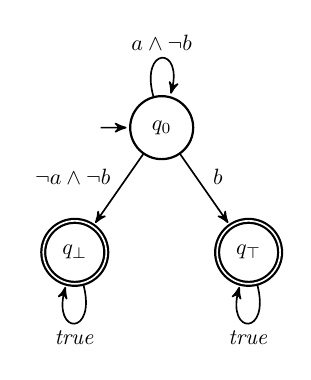
\begin{tikzpicture}[->,>=stealth',shorten >=1pt,auto,node distance=2.8cm,
semithick, scale=0.8, every node/.style={scale=0.8}, initial text={},
font=\normalsize]
   \tikzstyle{state}=[circle,thick,draw=black,fill=none,minimum size=10mm]
\node[state, accepting] (A)                    {$q_\bot$};
  \node[initial,state]         (B) [above right of=A, xshift= -6mm] {$q_0$};
  \node[state, accepting]         (C) [below right of=B, xshift= -6mm]
{$q_\top$};

 \path  (B) edge [loop above] node  {$a \wedge \neg b$} (B)
        (B) edge node [left, yshift=2mm] {$\neg a \wedge \neg b$}
(A)
        (B) edge node [right, yshift=2mm] {$b$} (C)
        (A) edge [loop below] node  {$\mathit{true}$} (A)
        (C) edge [loop below] node  {$\mathit{true}$} (C);
\end{tikzpicture} 

   \caption{\LTLtri monitor for $\varphi = a \, \U \, b$.}
    \end{figure}
   \label{fig:LTL3}
%\todo{Place this in a figure environment.}

%\section{Decentralized Synchronous Monitoring }
%\label{sec:synch}



\subsection{RV-LTL}


\RVLTL \cite{bls10}, which we will denote in this thesis by \LTLfour, refines 
the truth value ? into $\bot_p$ and~$\top_p$. That is, 
$\mathbb{B}_4=\{\top,\TT,\FT,\bot\}$. More specifically, evaluation of 
a formula in \LTLfour agrees with \LTLtri if the verdict is $\bot$ or 
$\top$. Otherwise, (i.e., when the verdict in \LTLtri is ?), \LTLfour 
utilizes \FLTL to compute a more refined truth value.

Now, let $\fintrace \in \alphabet^{*}$ be a finite trace. The truth value of an 
\LTLfour formula $\varphi$ with respect to $\fintrace$, denoted by $[\fintrace 
\models_4 \varphi]$, is defined as follows:
\begin{equation*}
 	\left[\fintrace \models_{4} \varphi \right] = 
 		\begin{cases} \top & \text{if }~~~~~[\fintrace \models_3 
\varphi] = \top\\
 		\bot & \text{if }~~~~~[\fintrace \models_3 \varphi] = 
\bot\\
 		\TT & \text{if }~~~~~[\fintrace \models_3 \varphi] =? \; \wedge 
\; [\fintrace \models_F \varphi] = \top\\ 

 		\FT & \text{if }~~~~~[\fintrace \models_3 \varphi] =? \; \wedge 
\; [\fintrace \models_F \varphi] = \bot\\ 
 	\end{cases}
 \end{equation*}



\begin{figure}[H]
\centering
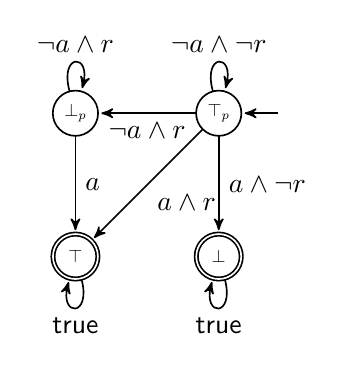
\begin{tikzpicture}[->,>=stealth',shorten >=1pt,auto,node distance=2.8cm,
                    semithick, initial text={}, initial where=right]
  \tikzstyle{every state}=[scale=0.65, every node/.style={scale=0.65}]

  \node[initial,state] (A)                {$\top_p$};
  \node[state]         (B) [left of  = A] {$\bot_p$};
  \node[state, accepting]         (D) [below of = B] {$\top$};
  \node[state, accepting]         (C) [below of = A] {$\bot$};

  \path (A) edge              node {$\neg a \wedge r$} (B)
            edge              node {$a \wedge \neg r$} (C)
            edge [loop above] node {$\neg a \wedge \neg r$} (A)
            edge              node {$a\wedge r$} (D)
        (B) edge [loop above] node {$\neg a \wedge r$} (B)
            edge              node {$a$} (D)
        (C) edge [loop below] node {$\tru$} (D)
        (D) edge [loop below] node {$\tru$} (D);


\end{tikzpicture}     \caption{\LTLfour monitor of $\varphi_{ra}$.}
\end{figure}
  \label{fig:RVltl}





 
 
The \LTLfour~{\em monitor} of a formula $\varphi$ is the unique deterministic 
finite state machine $\monitor^{\varphi}_4 = \{ \alphabet, Q, q_0, \delta, 
\lambda\}$, where $Q$ is a set of states, $q_0$ is the initial state, $\delta: Q 
\times \alphabet \to Q$ is the transition function, and $\lambda: Q 
\rightarrow \mathbb{B}_4$, is a function 
such that:
\[
\lambda(\delta(q_0, \fintrace)) = \left[\fintrace\models_4 \varphi\right]
\]
for every finite trace $\fintrace  \in \alphabet^*$.
%\qed
% \end{definition}
%
In \cite{bls11} , the authors introduce an algorithm that takes as input an \LTL 
formula and constructs as output an \LTLfour monitor. For example, 
Fig. 3.2 shows the \LTLfour monitor for the 
request/acknowledgement formula 
$\varphi_{ra} = \G(\neg a \wedge \neg r) \; \vee \, [(\neg a \, \U \, r) 
\,\wedge \, \F a]$.








          
        % \setcounter{figure}{0}
       % \setcounter{equation}{0}
       % \setcounter{table}{0}


 
\chapter{Decentralized Automata-Based Monitoring}
\label{chap:extended monitor}

An \LTLtri monitor can evaluate an \LTL formula $\varphi$ in a centralized 
setting where each proposition represents the global state of the system. We 
show in Section \ref{sec:DSM} and Chapter \ref{chap:DAM} that in a framework of several synchronous or asynchronous 
{\em unreliable} monitors, naive local monitoring may lead to inconsistent 
global verdicts for $\varphi$. More specifically, the set of verdicts emitted by 
the monitors may not be sufficient to distinguish executions that violate the 
formula from those that satisfy it. Intuitively, this is because each monitor 
has only a partial view of the system under inspection, and after a finite 
number of rounds of communication among monitors, still many different 
perspectives about the global system state remain. We use the \LTL formula 
$\varphi = \F (a \wedge b)$ throughout this Chapter to explain the concepts.

This Chapter is organized as follows: We discuss the synchronous monitoring problem in a failure-prone distributed environment in Section \ref{sec:DSM}. The model of computation and terminology are discussed in Section \ref{sec:modelterm}. The problem statement is given in Section \ref{sec:PS}, and in Section \ref{sec:challenge} we discuss the challenges in synchronous monitoring. The synchronous automata-based monitoring is discussed in Section \ref{sec:SAM} where we introduce our automata-based monitoring algorithm, and present the algorithm to construct an \Exltl.



\section{Synchronous Monitoring Algorithm Sketch}
\label{sec:DSM}

In this section, we propose a framework for synchronous distributed 
fault-tolerant runtime verification (RV). To this end, we make a link between 
RV and consensus in a failure-prone distributed environment by 
proposing an automata-based algorithm.

We consider a distributed monitoring system made up of a fixed number $n$ of 
monitors $\monitor = \{M_1, M_2, \dots, M_n\}$ that communicate by sending and 
receiving messages through point-to-point bidirectional communication links. 
Each communication link is reliable, that is, we assume no loss or alteration 
of messages. Each monitor locally executes an identical sequential algorithm. 
Each run of a monitor consists of a sequence of rounds that are identified by 
the successive integers 1, 2, etc. The round number is a global variable and 
its progress is ensured by the synchrony assumption. Each round is made up of 
three consecutive steps: {\em send}, {\em receive}, and {\em local 
computation}. The principle property of the round-based synchronous model is the 
fact that a message sent by a monitor $M_i$ to another monitor $M_j$ during a 
round $r$ is received by $M_j$ at the very same round $r$.

Throughout this chapter, the system under inspection produces a finite trace 
$\fintrace = \state_0\state_1\cdots \state_k$, and is inspected with respect to 
an \LTL formula $\varphi$ by a set of synchronous distributed monitors. 

\subparagraph{Algorithm sketch:} For every $j\in [0,k-1]$, between each 
$\state_j$ and $\state_{j+1}$, each monitor:

\begin{enumerate}
\item reads the value of a subset of propositions in $\state_j$, which may 
result in a {\em partial} observation of $\state_j$; 

\item at every synchronous round, {\em broadcasts} a message containing its 
current observation of the underlying system, and then waits for messages from 
other monitors;

\item based on the messages received at each round, executes a local 
computation, updates its current observation by incorporating observations of 
other monitors, and composing the message to be sent at next round, and

\item finally evaluates $\varphi$ at the end of communication rounds and 
subsequently emits a \truthvalue~from $\mathbb{B}_3$. 
\end{enumerate}

The skeleton of the algorithm is shown in Algorithm~\ref{alg:localmonalgo}.


\begin{algorithm}[H]

\small
\KwData{\LTL formula $\varphi$ and state $\state_j$}
\KwResult{a verdict from $\mathbb{B}_3$}
%$j = 0$\;
%\While{\rm there is a new state $s_j$}{
Let $\sample_i^{s_j}$ be the initial concrete local state of the monitor  

$LS_i^1 \gets$ $\mu (\sample_i^{s_j}, \varphi)$  \tcc*[r]{\it computes the initial abstract local state based on the initial concrete local state}

\For{\rm $r = 1,2, \cdots$ }  {  
{\em \textbf{Send:}}  broadcasts its current abstract local state $LS_i^r$ \tcc*[r]{\it $r$ is the round number}
\label{line:send} 
{\em \textbf{Receive:}} let $\Pi_i^r =$ $\{ LS_j^r\}_{j \in [1, n]}$ be the set of all messages received at round $r$. 


{\it \textbf{Computation:}}  $LS_i^{r+1} \gets$   $LC(\Pi_i^r)$ \tcc*[r]{\it calculates a new abstract local state} \label{line:computation} 

}
emits a verdict from $\mathbb{B}_3$ \tcc*[r]{\it evaluates $\varphi$ according to the final abstract local state}
\label{line:emit}
\caption{Behavior of Monitor $M_i$, for $i\in [1, n]$}
\label{alg:localmonalgo}
 \end{algorithm}












\section{Model of Computation and Terminology}
\label{sec:modelterm}
We now present our computation model, notation, and terminology.

\begin{definition}
\label{def:concretestate}
A `concrete local state' $\sample_i^{s_j}$ of a monitor $M_i$ at global 
state $s_j$ is a mapping from the set $\AP$ of atomic propositions to the set 
$\{\tru, \fals, \udef\}$, where $\udef$ denotes an unknown value, and for all 
$\ap \in \AP$, we have:
$$(\sample_i^{s_j}(\ap) = \tru \, \rightarrow \, ap \in s^j) \; \wedge \; 
(\sample_i^{s_j}(\ap) = \fals \, \rightarrow \, ap \not \in s_j)$$ 
\end{definition}

When a state $s_j$ is reached in a finite trace $\fintrace 
=\state_0\state_1\cdots \state_k$, each monitor $M_i \in \monitor$, for $1 \leq 
i \leq n$, takes a sample from $s_j$, which results in obtaining a concrete 
local state $\sample_i^{s_j}$. Hence, in the concrete local state of a monitor, 
if the value of an atomic proposition is not unknown, then its value is 
consistent with state $s_j$. Thus, two monitors $M_i$ and $M_l$ cannot have 
inconsistent concrete local states. That is, for any state $s_j$ and concrete 
local states $\sample_i^{s_j}$, $\sample_l^{s_j}$, and for every $\ap \in \AP$, 
we have:
$$(\sample_i^{s_j}(\ap) \neq \sample_l^{s_j}(\ap) \;  \rightarrow \; 
(\sample_i^{s_j}(\ap) = \udef \, \vee \, \sample_l^{s_j}(\ap) = \udef)$$

\begin{definition}
\label{def:abs}
An `abstract local state' $\abstate_i$ is a symbolic representation of a 
monitor $M_i$'s concrete local state $\sample_i^{\state_j}$ with respect to an \LTL formula 
$\varphi$ computed by an `abstraction function' $\mu$, where $\abstate_i = \mu 
(\sample_i^{\state_j}, \varphi)$.
\end{definition}

Note that Definition~\ref{def:abs} does not prescribe a specific symbolic 
representation or abstraction function. We will present a choice for this 
function in Section ~\ref{sec:SAM}. The idea here is that monitors communicate 
their abstract local states rather than concrete local states for space and 
communication efficiency. During the computation step, the monitor computes the 
message that it will to broadcast during the next round. Let $\abstate_i^r$ 
denote the abstract local state of $M_i$ at the beginning of round $r$. In the 
local computation step, a monitor $M_i$ modifies its abstract local state 
according to the messages it has received from other monitors (including its own 
message). Let
$$\Pi_i^r = \big\{ \abstate_l^r\big\}_{l \in [1, n]}$$
be the set of all messages received by monitor $M_i$ during round $r$. 

\begin{definition}
The `local computation function' of a monitor $M_i$ is a function $\LC$ 
that computes $M_i$'s new abstract local state in each round $r$, given the set 
of messages $\Pi_i^r$ received in round $r$. Formally,
$$\abstate_i^{r+1} = LC(\Pi_i^r)$$
\end{definition}

Similar to abstraction function, we will describe local computation 
function in Section ~\ref{sec:SAM}. 

\subparagraph{State Coverage:}  We say that a set of monitors \emph{cover} a 
global state if and only if the collection of concrete local states of these 
monitors covers the value of all atomic propositions. The formal definition 
is given below.

\begin{definition}
\label{def:state coverage}
A set $\monitor = \{M_1, M_2, \dots, M_n\}$ satisfies `state coverage' for 
a state $\state$ if and only if for every $\ap \in \AP$, there exists $M_i\in 
\monitor$ such that $\sample_i^\state(\ap) \neq \udef$.
\end{definition}

\begin{definition}
We say monitor $M_i$ is `aware' of proposition $ap$ at round $r$, if: 

\begin{itemize}
\item $\sample_i^\state(\ap) \neq \udef$, or 
\item $M_i$ receives a message from a monitor $M_j$ at round $r' \in [1,r)$, 
where $M_j$ is aware of $ap$ at round $r'$. 
\end{itemize}

\end{definition}


\subparagraph{Fault Model:} In our setting, the fault model specifies that each 
monitor may fail by {\em crashing} (i.e., halt and never recover). We assume 
that up to $n-1$ monitors can crash, where $n = |\monitor|$. A monitor may 
crash at any round. To ensure the state coverage, we assume that, if there is a 
proposition $ap \in \AP$, such that at round $r$ monitor $M_i$ is the only 
monitor aware of $ap$, then the message sent by $M_i$ at round $r$, must be 
received by at least one non-faulty monitor in round $r$. 

Note that in order to weaken the latter condition, one might assume that each proposition $\ap \in \AP$ is read by sufficiently large number of local monitors such that it is ensured that at least one monitor which is aware of $\ap$ does not crash, e.g., by assuming that each proposition is read by at least $f+1$ monitors.


\section{Problem Statement}
\label{sec:PS}

Suppose $\fintrace = \state_0\state_1\cdots \state_k$ is a finite trace 
generated by the system under inspection, and $\varphi$ is an \LTL formula with 
respect to which we monitor the system. Each monitor $M_i \in \monitor$, $i \in 
[1, n]$, runs Algorithm \ref{alg:localmonalgo} as follows. For any given new 
state $s_j$, monitor $M_i$ first obtains an initial concrete local state by 
taking a sample from $s_j$ (cf. Line 1). Recall from Definition 
\ref{def:concretestate} that the value of an atomic proposition in a 
concrete local state is either $\tru$, $\fals$, or $\natural$. After obtaining 
the initial concrete local state, monitor $M_i$ computes the initial local 
state based on the initial concrete local state (cf. Line 2). After 
intialization, each monitor $M_i$ executes a sequence of send, receive, and 
computation actions (cf. Lines 4-6) for some a priori known number of rounds.  
In Line 4, monitor $M_i$ sends its current abstract local state to all other 
monitors in $\monitor$. In Line 5, it receives messages from other monitors and 
stores them (along with its own message) in a set $\Pi_i^r$. In line 6, which is 
the computation step, monitor $M_i$ computes and updates its abstract local 
state based on messages in $\Pi_i^r$. Finally, after a certain number of rounds, 
the for-loop ends, and $M_i$ evaluates $\varphi$ and emits a \truthvalue~from 
$\mathbb{B}_3$ based on its final abstract local state (cf. Line 7). Note that 
Algorithm \ref{alg:localmonalgo} is executed whenever a new global state is 
reached in $\fintrace$. 

Our formal problem statement is the termination requirement for Algorithm 
\ref{alg:localmonalgo}. Roughly speaking, we require that when a 
non-faulty monitor runs Algorithm~\ref{alg:localmonalgo} to the end, it should 
compute and emit a verdict that a centralized monitor that has global view of 
the system would compute. This termination condition is formally, the following
$$\forall i \in [1, n] : M_i~ \text{is non-faulty} \; \rightarrow \valuation_i 
= [\alpha \models_3 \varphi]$$ 
where $\valuation_i$ is the \truthvalue~emitted by monitor $M_i$ at the end of 
running Algorithm~\ref{alg:localmonalgo}.

\section{Challenges in Synchronous Monitoring}
\label{sec:challenge}

It is easy to see that our decentralized synchronous monitoring problem, 
described in Section~\ref{sec:PS}, is similar to the uniform consesus problem that was described in Section \ref{sec:introDSM}. It is also straightforward to verify that the lower bound on the number of rounds required to consistently monitor the system is $f+1$, where $f$ is the total number of crashes the system can tolerate. The proof would be similar to 
the proof of the lower bound on the number of rounds required for the consensus 
algorithm that copes with $f$ process crashes.





Compared to the processing capacity of monitors, the communication links are low 
bandwidth, and hence, the communication costs are of concern. The communication 
cost depends on the number of messages transmitted by monitors, and 
the size of these messages. An increase in the message size enforced by the 
algorithm is referred to as the message size overhead. And an increase in the 
number of messages that must be transmitted is called the network traffic 
overhead. 

The following example illustrates the worst case scenario in which $f+1$ rounds 
are required to distributedly monitor the system, where $f$ is the total number 
of faults tolerated. It also shows how message size can dramatically increase with the state space of the system under inspection. 

\subparagraph{Example:}

Let $\varphi = \F (a \, \wedge \, b)$, $\AP=\{a, b\}$, and $\monitor =\{M_1, 
M_2, M_3, M_4\}$. Suppose $s=\{a,b\}$ is the current global state of the 
system, and the initial concrete local states of the monitors are as follows:
\begin{alignat*}{2}
& \sample^s_1[1](a)= \tru ~~~~~~~~~& \sample^s_1[1](b)=\natural\\
& \sample^s_2[1](a)= \natural & \sample^s_2[1](b) = \tru \\
& \sample^s_3[1](a) = \natural & \sample^s_3[1](b) =\natural \\ 
& \sample^s_4[1](a) = \natural & \sample^s_4[1](b) =\natural
%$\sample^s_5[1](a) =\natural$, $\sample^s_5[1](b) =\natural$ \\
\end{alignat*}
where $\sample^s_i[r]$ represents the concrete local state of monitor 
$M_i$ at the begining of round $r$. Let $f = 2$, i.e., at most $2$ 
monitors may crash, and suppose $M_1$ and $M_2$ are faulty monitors. The 
worst case scenario is when one and only one monitor crashes at each round. 
Suppose $M_1$ crashes at round $1$ and $M_2$ crashes at round $2$. Since $M_1$ 
is the only monitor that is aware of proposition $a$, according to our failure 
model assumption (in order to preserve the state coverage), at least one 
non-faulty monitor must receive a message from $M_1$ at round $1$. Let $M_2$ be 
the monitor that receives $M_1$'s message at round $1$.

According to Algorithm \ref{alg:localmonalgo}, the monitors are to broadcast 
their current abstract local states at each round. In this case, let the 
abstract local state of each monitor be the same as its concrete local state, 
i.e.,  $LS^r_i = \mu (\sample^s_i[r], \varphi) = \sample^s_i[r]$ where  
$\sample^s_i[r]$ is the concrete local state of monitor $M_i$ at round $r$. 
In this case, each message sent by a monitor is a {\em register} that consists 
of $|\AP|$ elements, one for each atomic proposition in $\AP$. At the end of 
each round, each monitor $M_i$ reads the values of all received messages and 
copies them into its local register as follows:
$$\forall p \in AP: (   (\sample_i^s[r](p) = \natural) \, \wedge \, (\exists j 
\in[1,n]:  \sample_j^s[r](p) \neq \natural) ) \; \rightarrow \;
(\sample_i^s[r](p) \gets \sample_j^s[r](p))$$
Hence, at the end of round $1$ (i.e., begining of round $2$), the concrete 
local states are as follows:
\begin{alignat*}{2}
&\sample^s_2[2](a)=\tru ~~~~~~~~~& \sample^s_2[2](b) = \tru \\
&\sample^s_3[2](a) =\natural & \sample^s_3[2](b) = \tru \\
&\sample^s_4[2](a) =\natural & \sample^s_4[2](b) =\tru
%$\sample^s_5[2](a) =\natural$, $\sample^s_5[2](b) =true$ \\ 
\end{alignat*}

Suppose monitor $M_2$ crashes at round $2$ and since it is the only monitor 
that is currently aware of proposition $a$, at least one non-faulty monitor 
must receive a message from $M_2$ at round $2$, suppose $M_3$ is the monitor 
which receives the message.  Thus, the new concrete local states at the end of 
round $2$ are as follows:
\begin{alignat*}{2}
&\sample^s_3[3](a) = \tru ~~~~~~~~~~& \sample^s_3[3](b) = \tru \\ 
&\sample^s_4[3](a) = \natural & \sample^s_4[3](b) = \tru
%$\sample^s_5[3](a) =\natural$, $\sample^s_5[3](b) =true$ \\
\end{alignat*}

Finally, at round $3$, since there is no faulty monitor, each monitor receives 
messages from all other monitors, and the concrete local states at the end of 
this round will be as follows:
\begin{alignat*}{2}
&\sample^s_3[4](a) = \tru ~~~~~~~& \sample^s_3[4](b) = \tru \\ 
&\sample^s_4[4](a) = \tru & \sample^s_4[4](b) = \tru
%$\sample^s_5[4](a) =true$, $\sample^s_5[4](b) =true$ \\
\end{alignat*}
Hence, at the end of round $3$ (namely., round $f+1$) all non-faulty monitors are aware 
of all propositions in $\AP$, and they emit the correct \truthvalue:

$$\valuation_3 = \valuation_4 = [\{a,b\} \models_3 \varphi] = \top$$
The following tables summarize the scenario: \\

\begin{tabular}{| c |c |c|}
\multicolumn{3}{c}{sample} \\
\hline
&$a$&$b$\\
\hline
$M_1$ & $\tru$  & $\natural$\\
$M_2$ & $\natural$ & $\tru$\\
$M_3$ & $\natural$ & $\tru$ \\
$M_4$ & $\natural$ & $\tru$ \\
%$M_5$ & $\natural$ & $true$ \\
\hline
\end{tabular}
\quad
\begin{tabular}{| c |c |c|}
\multicolumn{3}{c}{round 1} \\
\hline
&$a$&$b$\\
\hline
$M_1$ & crashed & crashed\\
$M_2$ & $\tru$ & $\tru$\\
$M_3$ & $\natural$ & $\tru$ \\
$M_4$ & $\natural$ & $\tru$ \\
%$M_5$ & $\natural$ & $true$ \\
\hline
\end{tabular}
\quad
\begin{tabular}{|c |c |c|}
\multicolumn{3}{c}{round 2} \\
\hline
&$a$&$b$\\
\hline
$M_1$ & crashed & crashed\\
$M_2$ & crashed & crashed\\
$M_3$ & $\tru$ & $\tru$ \\
$M_4$ & $\natural$ & $\tru$ \\
%$M_5$ & $\natural$ & $true$ \\
\hline
\end{tabular}

\begin{tabular}{| c |c |c|}
\multicolumn{3}{c}{round 3} \\
\hline
&$a$&$b$\\
\hline
$M_1$ & crashed & crashed\\
$M_2$ & crashed & crashed\\
$M_3$ & $\tru$ & $\tru$  \\
$M_4$ & $\tru$ & $\tru$  \\
%$M_5$ & $true$ & $true$  \\
\hline
\end{tabular}   

\ \\

%\todo{Please check $\valuation$ and $\verdict$}
%here talk about the message size in case of sending concrete local state.

One can see in the above example, in case each monitor broadcasts its concrete 
local state, namely, if the abstract local state is the same as the concrete 
local state, then each message sent by a monitor is a register that consists of 
$|\AP|$ elements, one for each atomic proposition in $\AP$. Our goal is to 
decrease the message size overhead, hence we introduce an algorithm that 
decreases the message size from $|\AP|$ bits to something 
significantly lower. In Section \ref{sec:SAM}, we introduce an algorithm which 
decreases the message size overhead in synchronous distributed monitoring. The 
algorithm solves the synchronous distributed monitoring problem in $f +1$ 
rounds of communication with message size of $\log(m_\monstate)$, where $m_\monstate$ is the number of outgoing transitions from monitor state $\monstate$ in an \Exltl~that will be introduced in Section \ref{sec:SAMExltl}.


\section{Synchronous Automata-based Monitoring}
\label{sec:SAM}

In this section, we introduce an automata-based algorithm that solves the 
decentralized synchronous monitoring problem in $f+1$ rounds of communication, 
where $f$ is the maximum number of crash failures tolerated. To this end, 
first, in Section~\ref{sec:SAMltl3}, we introduce an algorithm that is used by 
each local monitor to synchronously monitor the system under inspection. The 
general idea is that each local monitor evaluates the input formula and 
computes a {\em possible} set of verdicts, as a monitor may not know the 
value of all propositions. Then, through synchronous communication, the 
monitors share their verdict sets with each other. Finally, applying some 
function on the verdicts sets (e.g., computing their intersection) computes 
the verdict that a centralized monitor that has the global view of the system 
would compute.

Our algorithm uses \LTLtri monitor $\monitor^\varphi$ for a formula $\varphi$ in 
order to generate the set of possible verdicts. Thus, in our first attempt, in 
Section~\ref{sec:SAMltl3}, we use the \LTLtri monitors in our algorithm, but we 
also show that $\monitor^\varphi$, as defined in Section~\ref{sec:ltl3}, is 
not sufficient to consistently monitor the system for \LTL formulas. Then, 
in Section~\ref{sec:SAMExltl}, we introduce an `\Exltl' which we will use in 
each local monitor's algorithm to consistently monitor the global state of the 
system with respect to any \LTL formula. 



Note that in this work, we only consider monitoring of properties that are 
specified as \LTL formulas, as Pnueli’s \LTL \cite{p77} is a well-accepted 
linear-time temporal logic for specifying properties of infinite traces. 
However, In runtime verification, our goal is to check \LTL properties given 
finite prefixes of infinite traces. Therefore, one has to interpret their 
semantics with respect to finite prefixes as they arise in observing actual 
systems. Although it is possible to use infinite semantics of \LTL, namely by 
using nondeterministic B\"uchi automata as monitors and explore all 
nondeterministic choices, it is more convenient to use the finite semantics of 
\LTL to monitor \LTL formulas at run time. To this end, in \cite{bls11} 
introduced \LTLtri as a linear-time temporal logic which has the same syntax as 
in \LTL but deviates in its semantics for finite traces. To implement the idea 
that, for a given \LTLtri formula, its meaning for a prefix of an infinite trace 
must correspond to its meaning considered as an \LTL formula for the full 
infinite trace, they use three truth values: true, false, and inconclusive, 
denoted respectively by $\top$, $\bot$, and $?$.



\subsection{Synchronous Monitoring Using \LTLtri Monitors}
\label{sec:SAMltl3}

Recall that an \LTLtri monitor $\monitor^\varphi$ for \LTL formula $\varphi$ is 
a deterministic finite state machine (FSM) represented as $\monitor^\varphi = 
\{ \alphabet, Q, \monstate_0, \delta , \lambda \}$, where $\alphabet$ 
is a finite alphabet, $Q$ is a finite non-empty set of states (we refer to them 
as monitor states), $\monstate_0$ is the initial monitor state, $\delta: Q 
\times \alphabet \rightarrow 2^Q $ is a transition function, and $\lambda : Q 
\rightarrow \mathbb{B}_3 $ is a mapping function which maps each monitor state 
to a truth value in $\mathbb{B}_3=\{\top,\bot, ?\}$.

Observe that a transition $t_j^i$ from monitor state $\monstate_i$ to monitor 
state $\monstate_j$ is the set of all \events~$\state \in \alphabet $ such that 
$\delta (\monstate_i, \state) = \monstate_j$. More formally
$$ t_j^i = \{ \state \in \alphabet ~ | ~ \delta (\monstate_i, \state) = 
\monstate_j\}$$
Now, let $\monitor^\varphi$ be the \LTLtri monitor for an \LTL 
formula $\varphi$. We denote by $T_\monstate$ the set of all outgoing 
transitions from monitor state $\monstate$.  Formally, $T_\monstate =\{ 
t_1^\monstate, \cdots , t_{m_\monstate}^\monstate\}$ where $m_\monstate$ is the 
total number of outgoing transitions from monitor state $\monstate$ and each 
$t_j^\monstate$ is an outgoing transition from monitor state $\monstate$. Given 
that an \LTLtri monitor is a deterministic FSM, the followings hold 

\begin{itemize}
 \item $\forall j \in [1 \cdots m_\monstate]: t_j^\monstate \subseteq 
\alphabet$,
  \item $\forall j,k \in [1 \cdots 
m_\monstate]: j \neq k \Rightarrow  ~  t_j^\monstate \cap t_k^q = \emptyset$, and
  \item $t_1^\monstate \cup \cdots \cup t_{m_\monstate}^\monstate = \alphabet$.
\end{itemize}
%\renewcommand\labelitemi{-}


Let $\sample_i^s$ be the concrete local state of a monitor $M_i$ at global 
state $s$. We denote the set of all possible global \events~from the viewpoint 
of monitor $M_i$ by $\pevent(\sample_i^s)$:
\begin{center}
$\pevent(\sample_i^s) = \big\{ \state' \in \alphabet ~|~ \forall ap \in \AP: 
(\sample_i^s(ap) \neq \natural) \rightarrow ( (\sample_i^s(ap) = \tru 
\rightarrow ap \in \state') \wedge  (\sample_i^s(ap) = \fals \rightarrow ap 
\notin \state') ) \big\} $
\end{center}

Informally, $\pevent(\sample_i^s)$ is the set of all states $\state' \in 
\alphabet$ that are possible to be the global state $\state$, from viewpoint of 
monitor $M_i$. Obviously, for any global state $s$, we have: 
$$\forall i \in [1, n].~ s \in \pevent(\sample_i^s)$$

Now, suppose \LTLtri monitor $M_i$ is at state \monstate, and 
$\sample_i^s$ is $M_i$'s concrete local state. We denote the set of {\em 
possible verdicts} by monitor $M_i$ as follows
$$\verdict_i = \{\delta(\monstate, \state') \mid \state' \in 
\pevent(\sample_i^\state)\}$$
It should be noted that each verdict $v_j$ from a verdict set $\verdict_i$ is a 
monitor state. The mapping function $\lambda$ shall be applied to obtain the 
truth value of a verdict, i.e., $\lambda(v_j) \in \mathbb{B}_3$. Moreover, note 
that due to the synchrony assumption, all monitors always are at the same 
monitor state. Obviously, if all monitors are at monitor state $\monstate$ and 
the new global state of the system is $\state$, then we have
$$\forall i \in [1, n].~ \delta(\monstate, \state) \in \verdict_i$$

\subparagraph{Notation:} Let $\monstate$ be the current monitor state. We 
denote by $\intersection$ the intersection of all verdict sets emitted by 
all monitors in $\monitor$. Formally
$$ \intersection = \bigcap_{i = 1}^n  \verdict_i$$ 

Obviously, at every monitor state $\monstate \in Q$, we have $\delta(\monstate, 
\state) \in \intersection$, where $\state$ is a global state of the system. If
$|\intersection| =1$, then we have $\intersection = \{\delta(\monstate, 
\state)\}$. This case happens, when the set of all possible states of at least 
one monitor consists of only one state. In this case, the intersection 
represents the verdict of a centralized monitor that has global view of the 
system. This is formalized in the following lemma.

\begin{lemma} 
\label{lem:fullinfo}
Let $\state$ be a global state of the system and $\monstate$ be the current 
monitor state. If there is at least one monitor $M_i$ such that $\forall p \in 
\AP. ~ \sample_i^\state(ap) \neq \natural$, then we have $|\intersection| = 1$.
\end{lemma}

\begin{proof} 
It is easy to verify that if there is a monitor $M_i$ such that $\forall p \in 
\AP. \sample_i^\state(ap) \neq \natural$, then according to our definition, we 
have $\pevent(\sample_i^\state) = \{\state\}$. Consequently, we have 
$\verdict_i =  \{\delta(q, \state)\}$ and it follows that $|\intersection| = 
1$.
\end{proof}


\subparagraph{Abstraction Function in Automata-Based Algorithm.} Here we define 
the abstract local state $\abstate_i$ of a monitor $M_i$ to be the verdict set 
$\verdict_i$ emitted by the monitor. Given the concrete local state 
$\sample_i^\state $ of a monitor $M_i $ and the \LTLtri monitor 
$\monitor^\varphi$ of an \LTL formula $\varphi$, the abstraction function first 
computes the set of possible global states $\pevent(\sample_i^\state)$ from 
viewpoint of monitor $M_i$, and then calculates the verdict set based on 
$\pevent(\sample_i^\state)$. More formally

\begin{tabbing}
\= $\abstate_i = \absfunc_2(\pevent(\sample_i^\state), \monitor^\varphi) = \{\delta(\monstate, 
\state')\}_{\state' \in \pevent(\sample_i^\state)} = \verdict_i$ \\
\> $\pevent(\sample_i^\state) = \absfunc_1(\sample_i^\state) = $ \= $\{ \state' \in \alphabet \mid \forall ap \in \AP: 
(\sample_i^s(ap) \neq \natural) \rightarrow$\\
\>\> $( (\sample_i^s(ap) = \tru \rightarrow ap \in \state') \wedge  
(\sample_i^s(ap) = \fals \rightarrow ap \notin \state') ) \}$
\end{tabbing}
where $\absfunc_1$ and $\absfunc_2$ are the abstraction functions. $\absfunc_1$ receives as input a concrete local state $\sample_i^\state$ and computes the set of all possible global states $\pevent(\sample_i^\state)$, and $\absfunc_2$ receives as input a set of global states and a monitor $\monitor_\varphi$, and returns the set of all monitor states in $\monitor_\varphi$ that can be reached by the given global states.


\subparagraph{Local Computation Function in Automata-Based Algorithm.}The 
local computation function $LC$ of a monitor $M_i$ calculates the intersection 
of the messages (which are the verdict sets emitted by nonfaulty monitors) 
received in $\Pi_i^r$, at each round $r$. Formally,
$$\abstate_i^{r+1} = LC(\Pi_i^r) = \bigcap_{j \in [1, n]} \{ \abstate_j^r\} = 
\bigcap_{j \in [1, n]} \{\verdict_j^r\}$$

\subsection{Detailed Description of The Algorithm}

Each local monitor $M_i \in \monitor$, $i \in [1, n]$, runs Algorithm 
\ref{alg:localmonalgo2} that we shall describe in detail. For any given new 
state $s_j$, monitor $M_i$ first obtains an initial concrete local state by 
taking a sample from $s_j$ (cf. Line \ref{line:init2}). Recall 
from Definition \ref{def:concretestate} that the value of an atomic proposition 
in a concrete local state is either $\tru$, $\fals$, or $\natural$. After 
obtaining the initial concrete local state, monitor $M_i$ computes the initial 
abstract local state based on the initial concrete local state, by applying the 
abstraction functions $\mu_1$ and $\mu_2$ (cf. Line 
\ref{line:abst2}). After initialization, each 
monitor $M_i$ executes a sequence of send, receive, and computation actions (cf. 
Lines \ref{line:send2}-\ref{line:computation2}) for $f +1$ number of rounds.  In 
Line \ref{line:send2}, monitor $M_i$ sends its current local state to all other 
monitors in $\monitor$. In Line \ref{line:rec2}, it receives messages from other 
monitors and stores them, along with its own message, in a set $\Pi_i^r$. In 
line \ref{line:computation2}, which is the computation step, monitor $M_i$ 
computes and updates its abstract local state based on the messages in 
$\Pi_i^r$, by applying the local computation function $LC$ which simply 
calculates the intersection of the verdict sets in  $\Pi_i^r$. Finally, after 
$f+1$ rounds, the for-loop ends, and $M_i$ emits $\lambda(v_i) \in 
\mathbb{B}_3$, where $\{v_i\} = LS_i^{f+2}$(cf. Line \ref{line:emit2}). \\



\begin{algorithm}[H]

\small
\KwData{\LTLtri monitor $\monitor^\varphi$ and state $\state_j$}
\KwResult{a verdict from $\mathbb{B}_3$}
\DontPrintSemicolon
%$j = 0$\;
%\While{\rm there is a new state $s_j$}{
Let $\sample_i^{s_j}$ be the initial concrete local state of the monitor  \label{line:init2}

$LS_i^1 \gets$ $\mu_2 (  \mu_1(\sample_i^{s_j}, \monitor_\varphi)) = \verdict_i^1$  \tcc*[r]{\it computes the initial abstract local state based on the initial concrete local state. $\verdict_i^r$ denotes the verdict set emitted by monitor $M_i$ to be broadcasted at round $r$}   \label{line:abst2}

\For{\rm $r = 1, \cdots , f +1 $  }  {   \tcc*[r]{\it $f$ is the maximum number of crash failures tolerated}
{\em \textbf{Send:}}  broadcasts its current abstract local state $LS_i^r = \verdict_i^r$ \tcc*[r]{\it $r$ is the round number}
\label{line:send2} 
{\em \textbf{Receive:}} let $\Pi_i^r =$ $\{ \verdict_j^r\}_{j \in [1, n]}$ be the set of all messages received at round $r$. \label{line:rec2}

{\it \textbf{Computation:}}  $LS_i^{r+1} \gets LC_i(\Pi_i^r) = \bigcap_{j \in [1, n]} \{\verdict_j^r\}$ \tcc*[r]{\it calculates a new abstract local state} \label{line:computation2} 

}
emit $\lambda_e(v_i)$  \tcc*[r]{\it where $ \{v_i\} = LS_i^{f +2}$}
\label{line:emit2}
\caption{Behavior of Monitor $M_i$, for $i\in [1, n]$}
\label{alg:localmonalgo2}
\end{algorithm}










 \ \ \ \

Now let us look at the following example to see how each local monitor 
implements Algorithm \ref{alg:localmonalgo2} to emit a verdict. In the following 
example each monitor employs \LTLtri monitor $\monitor^\varphi$ of a given \LTL 
formula $\varphi$, in order to compute an abstract local state based on its 
concrete local state. 

\textbf{Example:} Let $\varphi = \F (a \wedge b)$ 

\begin{figure}[H]
\centering
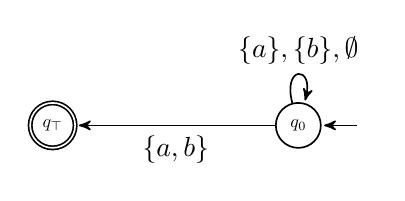
\begin{tikzpicture}[->,>=stealth',shorten >=1pt,auto,node distance=4.8cm,
                    semithick, initial text={}, initial where=right]
  \tikzstyle{every state}=[scale=0.65, every node/.style={scale=0.65}]

  \node[initial,state] (A)                {$\monstate_0$};
  \node[state, accepting]         (B) [left of  = A] {$\monstate_\top$};

  \path (A) edge              node {$ \{a,b\}$} (B)
 
            edge [loop above] node {$\{a\}, \{b\}, \emptyset$} (A) ;
        
\end{tikzpicture}    
\caption{\LTLtri monitor of $\varphi = \F(a \wedge b)$.}
\end{figure}

Consider $\monitor=\{M_1, M_2, M_3, M_4\}$, $s=\{a,b\}$, $S^s_1(a)=\tru$, 
$S^s_1(b)=\natural$, $S^s_2(a)=\natural$, $S^s_2(b)=\tru$, $S^s_3(a) 
=\natural$, $S^s_3(b) =\natural$,  $S^s_4(a) =\natural$, $S^s_4(b) =\natural$, 
and let $f=2$. According to Algorithm \ref{alg:localmonalgo2}, each local 
monitor $M_i$ computes an abstract local state $\abstate_i^1$ based on its 
concrete local state using abstraction functions $\mu_1$ and $\mu_2$ (cf. Line 
\ref{line:init2}). The initial abstract local states are given in Table below (sample).\\


\begin{tabular}{| c |c |c |c|}
\multicolumn{3}{c}{sample} \\
\hline
&$a$&$b$&$\abstate_i^1$\\
\hline
$M_1$ & $\tru$  & $\natural$ & $\{\monstate_0, \monstate_\top\}$\\
$M_2$ & $\natural$ & $\tru$ &  $\{\monstate_0, \monstate_\top\}$\\
$M_3$ & $\natural$ & $\natural$ &  $\{\monstate_0, \monstate_\top\}$ \\
$M_4$ & $\natural$ & $\natural$ &  $\{\monstate_0, \monstate_\top\}$\\
%$M_5$ & $\natural$ & $true$ \\
\hline
\end{tabular} 
\quad
\begin{tabular}{| c |c|}
\multicolumn{2}{c}{round 1} \\
\hline
&$\abstate_i^2$\\
\hline
$M_1$ & crashed\\
$M_2$ & $\{\monstate_0, \monstate_\top\}$\\
$M_3$ & $\{\monstate_0, \monstate_\top\}$ \\
$M_4$ & $\{\monstate_0, \monstate_\top\}$ \\
%$M_5$ & $\natural$ & $true$ \\
\hline
\end{tabular}
\quad
\begin{tabular}{| c |c|}
\multicolumn{2}{c}{round 2} \\
\hline
&$\abstate_i^3$\\
\hline
$M_1$ & crashed\\
$M_2$ & crashed\\
$M_3$ & $\{\monstate_0, \monstate_\top\}$ \\
$M_4$ & $\{\monstate_0, \monstate_\top\}$ \\
%$M_5$ & $\natural$ & $true$ \\
\hline
\end{tabular}
\quad
\begin{tabular}{| c |c|}
\multicolumn{2}{c}{round 3} \\
\hline
&$\abstate_i^4$\\
\hline
$M_1$ & crashed\\
$M_2$ & crashed\\
$M_3$ & $\{\monstate_0, \monstate_\top\}$ \\
$M_4$ & $\{\monstate_0, \monstate_\top\}$ \\
%$M_5$ & $\natural$ & $true$ \\
\hline
\end{tabular} \\ \\

$M_1$ knows that the value of proposition $a$ is true in \event~$\state$, but it 
does not know the value of proposition $b$ in $\state$. Therefore, from its 
viewpoint \event~$\state$ can be either $\{a\}$ or $\{a,b\}$. We say $\{a\}$ and 
$\{a,b\}$ are possible global \events~from veiwpoint of $M_1$. Thus $M_1$'s 
initial abstract local state is the verdict set $\abstate_1^1=\{\monstate_0, 
\monstate_\top \}$ which includes the monitor states that can be reached by 
\events~$\{a\}$ and $\{a,b\}$, as $\delta(\monstate_0, \{a\})=\monstate_0$ and 
$\delta(\monstate_0, \{a,b\})=\monstate_\top$. Similarly, the possible global 
\events~from viewpoint of monitor $M_2$ are $\{b\}$ and $\{a,b\}$, therfore its 
initial abstract local state is the verdict set $\abstate_2^1=\{\monstate_0, 
\monstate_\top \}$, which are the monitor states that can be reached by 
\events~$\{b\}$ and $\{a,b\}$. $M_3$ and $M_4$ do not know the value of any 
proposition in $\state$, thus from their viewpoint, all global states 
$\emptyset$, $\{a\}$, $\{b\}$, and $\{a,b\}$ are possible to be the global state 
$\state$, hence $\abstate_3^1= \abstate_4^1=\{\monstate_0, \monstate_\top\}$.

Suppose monitor $M_1$ crashes at round $1$ and since it is the only monitor 
which knows the value of proposition $a$, we assume its message is received by 
at least one nonfaulty monitor, e.g. $M_2$. Therefore, after one round of 
communication, each monitor updates its abstract local state by calculating the 
intersection of its own verdict set with the verdict sets received from other 
monitors (cf. Line \ref{line:computation2}): 

 $\abstate_2^2 = \{\monstate_0, \monstate_\top\}$,
 $\abstate_3^2 = \{\monstate_0, \monstate_\top\}$,
 $\abstate_4^2 = \{\monstate_0, \monstate_\top\}$ 
 
\noindent In round $2$, monitor $M_2$ crashes, and again, since it is the only 
monitor whose abstract local state encapsualtes proposition $a$, its message 
must be received by at least one monitor, e.g. $M_3$, at this round. The 
abstract local states at the end of round $2$ will be updated as follows: 

 $\abstate_3^3 = \{\monstate_0, \monstate_\top\}$,
 $\abstate_4^3 = \{\monstate_0, \monstate_\top\}$ 


\noindent Finally at round $3$, no monitor crashes and $M_4$ and $M_3$ receive 
messages from each other and update their abstract local states:

 $\abstate_3^4 = \{\monstate_0, \monstate_\top\}$,
 $\abstate_4^4 = \{\monstate_0, \monstate_\top\}$ \\

As we observe, at the end of round $3$ (namely, $f+1$), the local monitors still 
cannot decide a single verdict since $|\abstate_i^4| > 1$. This is because the 
\LTLtri monitor of $\varphi = \F (a \wedge b)$ is not sufficient to distinguish 
the correct verdict when local monitors have partial view of the system. In 
particular, monitors $M_3$ and $M_4$ both have $\{\monstate_0, 
\monstate_\top\}$ as their verdicts, while $[\{a, b\} \models_3 \F(a 
\wedge b)] = \top$. That is, the monitors cannot map their collective verdicts 
to the verdict of a monitor that has the global view of the system. 


In order to resolve this insufficiency, we introduce an algorithm that 
constructs an `\Exltl'. The algorithm receives as input an \LTLtri monitor and 
solely based on the structure of the input monitor, it determines whether to add 
new monitor states to the original \LTLtri monitor. The \Exltl~then is used in 
each local monitor $M_i$'s algorithm (Algorithm \ref{alg:localmonalgo2}) to 
consistently solve the decentralized synchronous monitoring problem. As 
described earlier, the intuition behind this algorithm is to monitor the system 
under inspection by taking the intersection of the sets of verdicts emitted by a 
set of distributed monitors. 

\subsection{Synchronous Automata-Based Monitoring Using Extended \LTLtri 
Monitor}
\label{sec:SAMExltl}

In this Section, first we present an algorithm to construct an 
\Exltl~$\monitor_e^\varphi$ which can be used in Algorithm 
\ref{alg:localmonalgo2} to solve the synchronous monitoring problem that was 
described in Section \ref{sec:PS}, for any given \LTL formula $\varphi$. Then 
we provide an example to show how $\monitor_e^\varphi$ is used in each local 
monitor's algorithm to emit their verdicts and consistently monitor the system.

\subsubsection{Extended \LTLtri Monitor Construction}
\label{sec:ExltlConst}

Let $\monitor^\varphi=\{\Sigma, Q, \delta, \monstate_0, F\}$ be the \LTLtri 
monitor for \LTL formula $\varphi$. Our goal is to construct an 
\Exltl~$\monitor_e^\varphi =  \{ \alphabet, Q_e, \monstate_0, \delta_e , 
\lambda_e\}$ such that $|\intersection|=1$ at every monitor state $\monstate \in 
Q_e$, where $\intersection$ is the intersection of the verdict sets emitted by a 
set of distributed monitors whose partial views (namely, concrete local states) 
cover the global state of the system under inspection (see Definition 
\ref{def:state coverage}).

\begin{definition}
\label{def:Exltl}
Let $\monitor^\varphi = \{ \alphabet, Q, \monstate_0, \delta , \lambda\}$ be the 
\LTLtri monitor of an \LTL formula $\varphi$. An {\em \Exltl}~of $\varphi$ is a 
deterministic finite state machine $\monitor^\varphi_e = \{ \alphabet, Q_e, 
\monstate_0, \delta_e , \lambda_e\}$, where $Q_e$ is a set of states s.t. $Q 
\subseteq Q_e$, $q_0$ is the initial state, $\delta_e: Q_e \times \alphabet 
\rightarrow 2^{Q_e}$ is a transition function, and $\lambda_e : Q_e 
\rightarrow \mathbb{B}_3 $ is a mapping function, such that (1) for every 
non-empty finite trace $\alpha \in \alphabet^*$, we have $\lambda_e 
(\delta_e(q_0, \alpha)) = \lambda (\delta(q_0, \alpha))$, and (2) at every 
$\monstate \in Q_e$ we have $|\intersection| = 1$.
\end{definition}

Algorithm \ref{alg:extendedmonalg} constructs an \Exltl~given an \LTLtri monitor 
$\monitor^\varphi$. \\



%\newcommand\mycommfont[1]{\tiny\ttfamily\textcolor{black}{#1}}
%\SetCommentSty{mycommfont}
%\usepackage[skins]{tcolorbox}
%\begin{tcolorbox}[blanker,width=(\linewidth-0.0cm)]


\begin{algorithm}[H]
\tiny
\KwIn{$\monitor^\varphi = \{ \alphabet, Q, \monstate_0, \delta , \lambda\}$}
\KwOut{$\monitor^\varphi_e = \{ \alphabet, Q_e, \monstate_0, \delta_e , \lambda_e\}$}           

\DontPrintSemicolon
$Q_e \leftarrow Q$ \\   \label{line:initExl}
\For {every $\monstate_i \in Q$}{
 \label{line:everystate}
 Obtain the set of outgoing transitions $T_i $ from monitor state $\monstate_i$   \\
 \label{line:outgoingtrans}
% \While {$T_i \neq \emptyset$}   {
   \For {every $t_j^i \in T_i$} {     
  \label{line:everytrans}
   \tcc*[r]{\it $t_j^i = \{s \in \alphabet ~|~  \delta(\monstate_i, s) = \monstate_j \}$}  
  
   \tcc*[r]{\it $N_j$ denotes the number of transitions from which $t_j^i$ is \indist, and $K_j$ denotes the number of transitions \indist~from $t_j^i$}
      $N_j \leftarrow 0 ~,~  K_j \leftarrow 0$      \\ 
    \label{line:initNK}
     \For {every $t_k^i \in T_i \backslash \{t_j^i\}$ } {     \label{line:indisting}
      \If{\indisting($t_j^i$, $t_k^i)$}{  \label{line:indistingfrom}
       $N_j \leftarrow N_j + 1$}
      \If{\indisting($t_k^i$, $t_j^i)$}{  \label{line:fromindisting}
       $K_j \leftarrow K_j + 1$}   \label{line:indistingend}
     }
     \If{$N_j > 0$}{ \label{line:split0}
      $\{t_{j1}^i, t_{j2}^i\}  \leftarrow \splitt(t_j^i, N_j, K_j, T_i) $  \label{line:split}
      
      $T_i \leftarrow \{ t_{j1}^i, t_{j2}^i\}  \cup T_i \backslash \{t_j^i\}$\\    \label{line:T-update}      
      $Q_e \leftarrow \{\monstate_{j1}, \monstate_{j2}\} \cup (Q_e \backslash   \{\monstate_j\})$ \\  \label{line:monstate-update}
      
      \If{$i \neq j$}{     \label{line:delta-update0}
         \For {every $t_k^i \in T_i$}{  \label{line:delta-oldtrans0}
           $\delta(\monstate_i, \state) = \monstate_k$ for every $\state \in t_k^i$   
         }
         $\delta(\monstate_{j1}, \state) \leftarrow \delta(\monstate_i, \state)$ for every $\state \in \alphabet$ \\  \label{line:delta-newtrans01}
         $\delta(\monstate_{j2}, \state) \leftarrow \delta(\monstate_i, \state)$ for every $\state \in \alphabet$       \label{line:delta-newtrans02}
      }
      \If{$i = j$}{   \label{line:delta-update1}  
          \For {every $t_k^i \in T_i$}{ \label{line:delta-oldtrans1}
           $\delta(\monstate_{j1}, \state) = \monstate_k$ for every $\state \in t_k^i$ 
         }
          $\delta(\monstate_{j2}, \state) \leftarrow \delta(\monstate_{j1}, \state)$ for every $\state \in \alphabet$         \label{line:delta-newtrans1}
      }
      
      $\lambda_e(\monstate_{j1})\leftarrow \lambda(\monstate_j)$ \\ \label{line:lambda-update0}
      $\lambda_e(\monstate_{j2})\leftarrow \lambda(\monstate_j)$ \\  \label{line:lambda-update1}
     }  \Else {
    
    
      $\delta_e(\monstate_i, s) \leftarrow \monstate_j$ for every $\state \in t_j^i$ \\  \label{line:delta-update2}
      $\lambda_e(\monstate_j)\leftarrow \lambda(\monstate_j)$ \\   \label{line:lambda-update2}
     }
   }   
% }      
} 

\caption{\Exltl~Construction}
\label{alg:extendedmonalg}
\end{algorithm}
%\end{tcolorbox}

%\begin{tcolorbox}[blanker,width=(\linewidth-0.1cm)]
\begin{algorithm}[H]
\DontPrintSemicolon
%\SetNoFillComment
  
\begin{algorithmic}
\tiny
\Function{\textit{\splitt}}{transition $t_j^i, N_j, K_j$, set of transitions $T_i$} 
\State $N_{j, min} \leftarrow N_j$   
\State $K_{j, min} \leftarrow K_j$    %\tcc*[r]{\it$N_j$ and $K_j$ are calculated in Algorithm \ref{alg:extendedmonalg}}

%\State $  \partition(t_j)$
\State \For {every $\{t_{j1}^{i,l}, t_{j2}^{i,l}\} \in \partition(t_j^i)$ }{
              
    $N_{jl} \leftarrow 0 ~,~ K_{jl} \leftarrow 0$ \
            
    \For {every $t_k^i \in  (\{t_{j2}^{i,l}\} \cup T_i \backslash \{t_j^i\})$ } {    
                  \If{\indisting($t_{j1}^{i,l}$, $t_k^i)$}{
                   $N_{jl} \leftarrow N_{jl}+1$}                     
                   \If{\indisting($t_k^i$, $t_{j1}^{i,l})$}{         
                    $K_{jl} \leftarrow K_{jl}+1$}
     }              
     \For {every $t_k^i \in  (\{t_{j1}^{i,l}\} \cup T_i \backslash \{t_j^i\})$ } {    
                  \If{\indisting($t_{j2}^{i,l}$, $t_k^i)$}{
                   $N_{jl} \leftarrow N_{jl}+1$}
                   \If{\indisting($t_k^i$, $t_{j2}^{i,l})$}{
                    $K_{jl} \leftarrow K_{jl}+1$}
                  
    } 
    \If {$(N_{jl}+K_{jl}) \leqslant (N_{j,min}+K_{j,min})$} {
       $l_{min} = l$
    }         
}          


  $  t_{j1}^i =  t_{j1}^{i,l_{min}},  t_{j2} ^i = t_{j2}^{i, l_{min}}$
  

\Return $\{t_{j1}^i, t_{j2}^i\}$
\EndFunction
\end{algorithmic}   

\begin{algorithmic}
\tiny
\Function{\textit{\partition}}{transition $t_j^i$}
  \State  compute all partitions $\{t_{j1}^{i,l} , t_{j2}^{i,l}\}$ of $t_j^i$ where $l \in [1 \cdots \frac{2^{| t_j^i|}-2}{2}]$, s.t.  
 \State for every pair $\{t_{j1}^{i,l} , t_{j2}^{i,l}\}$: 
  
  \begin{itemize}
  \item $t_{j1}^{i,l} \cup  t_{j2}^{i,l} = t_j^i$
  \item $t_{j1}^{i,l} \cap  t_{j2}^{i,l} = \emptyset$
  \end{itemize}
 
 \Return $\{\{t_{j1}^{i,1} , t_{j2}^{i,1}\}, \{t_{j1}^{i2} , t_{j2}^{i2}\}, \cdots , \{t_{j1}^{i, 2^\frac{2^{| t_j^i|}-2}{2}} , t_{j2}^{i, \frac{2^{| t_j^i|}-2}{2}} \}  \}$

\EndFunction
\end{algorithmic}

\caption{Functions \splitt~and \partition}
\end{algorithm}
%\end{tcolorbox} 
 
 
 \iffalse
 
\begin{algorithm}[H]   

\begin{algorithmic}
\tiny
\Function{\textit{\partition}}{transition $t_j^i$}
  \State  compute all partitions $\{t_{j1}^{i,l} , t_{j2}^{i,l}\}$ of $t_j^i$ where $l \in [1 \cdots \frac{2^{| t_j^i|}-2}{2}]$, s.t.  
 \State for every pair $\{t_{j1}^{i,l} , t_{j2}^{i,l}\}$: 
  
  \begin{itemize}
  \item $t_{j1}^{i,l} \cup  t_{j2}^{i,l} = t_j^i$
  \item $t_{j1}^{i,l} \cap  t_{j2}^{i,l} = \emptyset$
  \end{itemize}
 
 \Return $\{\{t_{j1}^{i,1} , t_{j2}^{i,1}\}, \{t_{j1}^{i2} , t_{j2}^{i2}\}, \cdots , \{t_{j1}^{i, 2^\frac{2^{| t_j^i|}-2}{2}} , t_{j2}^{i, \frac{2^{| t_j^i|}-2}{2}} \}  \}$

\EndFunction
\end{algorithmic}


 \begin{algorithmic}
 \tiny
\Function{\textit{\indisting}}{transition $t_1$, transition $t_2$}
  \State \If {there exists $\state \in t_2$ s.t. $\dep(\state, t_1)$}{
     \Return True} \Else {\Return False}
\EndFunction
\end{algorithmic}   

\begin{algorithmic}
\tiny
\Function{\textit{\dep}}{\event~$\state$, transition $t$}
  \State \If {$(\forall ap \in AP.~ \exists \state' \in t.~ (ap \in \state \Leftrightarrow ap \in \state' ))$}{
     \Return True} \Else {\Return False}
\EndFunction
\end{algorithmic}


\caption{Functions \partition, \indisting, and \dep}
\end{algorithm}  \ \

\fi










 \ \ \ \


\subsubsection{Detailed Description of Algorithm \ref{alg:extendedmonalg}}

We now explain how Algorithm \ref{alg:extendedmonalg} constructs an 
\Exltl~$\monitor_\varphi$ from an \LTLtri monitor $\monitor^\varphi$. As 
described in Definition \ref{def:Exltl}, the goal is to construct a 
deterministic finite state machine $\monitor^\varphi_e = \{ \alphabet, Q_e, 
\monstate_0, \delta_e , \lambda_e\}$ such that $|\intersection| = 1$ at every 
monitor state $\monstate \in Q_e$. Algorithm \ref{alg:extendedmonalg} first 
initializes $Q_e$ with $Q$ (cf. Line \ref{line:initExl}). Then, for every 
$\monstate_i \in Q$, it obtains the set of all outgoing transitions from 
$\monstate_i$, which is denoted by $T_i$ (cf. Line \ref{line:outgoingtrans}). 
Recall that $t_j^i = \{\state \in \alphabet ~ | ~ \delta (\monstate_i, \state) 
= \monstate_j\}$ is a transition from monitor state $\monstate_i$ to  monitor 
state $\monstate_j$. Two variables $N_j$ and $K_j$ are associated to every 
transition $t^i_j \in T_i$ (cf. Line \ref{line:initNK}). $N_j$ keeps the number 
of transitions in $T_i$ from which transition $t^i_j$ is \indist, and $K_j$ keeps the 
number of transitions in $T_i$ that are \textit{\indist}~from transition 
$t^i_j$. The notion of `\indist' is defined in Definition \ref{def:indisting} below. In Lines 
\ref{line:indistingfrom}-\ref{line:indistingend}, the algorithm verifies for every 
transition $t^i_k \in T_i \backslash \{t^i_j\}$ whether $t^i_j$ is \indist~from 
$t^i_k$, and/or $t^i_k$ is \indist~form $t^i_j$, and updates $N_j$ and $K_j$, 
respectively. If $N_j = 0$ it means that $t_j^i$ is \textit{\dist} from all 
transitions in $T_i \backslash \{t_j^i\}$, thus there is no need to 
\splt~$t_j^i$, therefore the algorithm proceeds to Lines 
\ref{line:delta-update2}-\ref{line:lambda-update2}. In Lines 
\ref{line:delta-update2} and \ref{line:lambda-update2} transition function 
$\delta_e$ and mapping function $\lambda_e$ of the \Exltl~are updated by adding 
transitions $\delta_e(\monstate_i, \state) = \monstate_j , \forall \state  \in 
t_j^i$, and  the mapping $\lambda_e(\monstate_j) = \lambda(\monstate_j)$, 
respectively.

If $N_j > 0$ it means that there is at least one transition $t^i_k \in T_i 
\backslash \{t^i_j\}$ such that $t_j^i$ is \indist~from $t_k^i$. In this case, 
the Algorithm proceeds to Lines \ref{line:split}-\ref{line:lambda-update1}. in 
Line \ref{line:split} transition $t_j^i$ is splitted into two new transitions 
$t_{j1}^i$ and $t_{j2}^i$ by using the function \splitt. Function \splitt~ is 
described below. In Line \ref{line:T-update}, the new transitions $t_{j1}^i$ and 
$t_{j2}^i$  are added to the set of outgoing transitions $T_i$ from monitor 
state $\monstate_i$ and $t_j^i$ is removed from $T_i$. In Line 
\ref{line:monstate-update}, monitor state $\monstate_j$ is replaced by two new 
monitor states $\monstate_{j1}$ and $\monstate_{j2}$ in $Q_e$. The transition 
function $\delta_e$ is updated in Lines 
\ref{line:delta-update0}-\ref{line:delta-newtrans1}. If the transition $t_j^i$ 
is not a self-loop, i.e., $i \neq j$, then the transition function $\delta_e$ is 
updated through Lines \ref{line:delta-oldtrans0}-\ref{line:delta-newtrans02}. If 
$t_j^i$ is a self-loop, then $\delta_e$ is updated through Lines 
\ref{line:delta-oldtrans1}-\ref{line:delta-newtrans1}, where the monitor state 
$\monstate_i$ is practically replaced by $\monstate_{j1}$. Finally, in Lines 
\ref{line:lambda-update0}-\ref{line:lambda-update1}, the mapping function 
$\lambda_e$ is updated with the new mappings $\lambda_e(\monstate_{j1}) = 
\lambda(\monstate_j)$ and $\lambda_e(\monstate_{j2}) = \lambda(\monstate_j)$.

As mentioned earlier, when a transition $t_j^i$ is \splt ted into two 
transitions $t_{j1}^0$ and $t_{j2}^0$, consequently two new monitor states 
$\monstate_{j1}$ and $\monstate_{j2}$ are added to $\monitor_e^\varphi$. Note 
that $\monstate_{j1}$ and $\monstate_{j2}$ have the same mapping  and the same 
set of outgoing transitions as $\monstate_i$. Namely, $\lambda(\monstate_{j1}) 
= \lambda(\monstate_{j2}) = \lambda(\monstate_i)$, and $T_{j1} = T_{j2} = T_i$. 
This is in fact a necessary condition in order to have
$$ [\alpha \models_3 \varphi] =  [\alpha \models_3^e \varphi]  $$ where $ [\alpha \models_3^e \varphi] \in \mathbb{B}_3$ denotes the valuation of any finite trace $\alpha$ according to an \Exltl.

\begin{definition}
\label{def:covered}

We say state $\state$ is `covered' by transition $t$, and we denote it 
by $\dep(\state, t)$, if we have:
$$ \forall \ap \in \AP.~ \exists \state' \in t. ~(\ap \in \state 
\Leftrightarrow \ap \in \state') $$

\end{definition}


\begin{definition}
\label{def:indisting}
We say a transition $t_1$ is `indistinguishable' from another transition 
$t_2$, and denote it by $\indisting(t_1, t_2)$, if the following holds:
$$\exists \state \in t_2 . ~ \dep(\state, t_1)$$

Transition $t_1$ is \textit{\dist} from $t_2$, denoted by $\disting(t_1, t_2)$, if it is not \indist~form $t_2$.
\end{definition}


\subparagraph{Function \splitt} This function is in fact the main function in Algorithm \ref{alg:extendedmonalg}. Given a transition $t_j^i \in T_i$, it splits $t_j^i$ into two new transitions $t_{j1}^i$ and $t_{j2}^i$ such that the total number of transitions in $T_i \backslash \{t_j^i\}$ that are \indist~from $t_{j1}^i$ and transitions that are \indist~from $t_{j2}^i$, plus the total number of transitions in $T_i \backslash \{t_j^i\}$ from which $t_{j1}^i$ is \indist~and transitions from which $t_{j2}^i$ is \indist~is minimum. This is because we are interested in generating the minimum number of new transitions, and consequently minimum number of new monitor states. Hence, we can claim that an \Exltl~constructed by Algorithm \ref{alg:extendedmonalg} is optimum in the terms that $|Q_e|$ is minimum.
This is done as follows; first all \textit{\partitionn}s of $t_j^i$ are calculated by function \partition~which is described below. Two variables $N_{jl}$ and $K_{jl}$ are used in function \splitt~where $N_{jl}$ is a counter for the total number of transitions in $T_i \backslash \{t_j^i\}$ from which $t_{j1}^i$ is \indist, and transitions from which $t_{j2}^i$ is \indist. $K_{jl}$ is a counter for the total number of transitions in $T_i \backslash \{t_j^i\}$ that are \indist~from $t_{j1}^i$, and transitions that are \indist~from $t_{j2}^i$. Function \splitt~calculates $N_{jl} + K_{jl}$ for all \partitionn s $\{t_{j1}^{i,l}, t_{j2}^{i,l}\} \in \partition$ and returns a \partitionn~with minimum value of $N_{jl} + K_{jl}$. 




\subparagraph{Function \partition} Given a transition $t_j^i$, this function returns the set of all possible partitions $\{t_{j1}^i, t_{j2}^i\}$ such that:

\begin{itemize}
\item  $t_{j1}^i \cap t_{j2}^i = \emptyset$
\item  $t_{j1}^i \cup t_{j2}^i = t_j^i$
\end{itemize}

It is easy to verify that the total number of such \partitionn s is equal to $\frac{2^{|t_j^i|}-2}{2}$. 

Now we employ our \Exltl~in each local monitor's algorithm to consistently monitor the global state of the system. We replace the \LTLtri monitor $\monitor^\varphi$ in Algorithm \ref{alg:localmonalgo2} with an \Exltl. \\

%
\begin{algorithm}[H]

\small
\KwData{\Exltl~$\monitor_e^\varphi$ and state $\state_j$}
\KwResult{a verdict from $\mathbb{B}_3$}
\DontPrintSemicolon
%$j = 0$\;
%\While{\rm there is a new state $s_j$}{
Let $\sample_i^{s_j}$ be the initial concrete local state of the monitor  

$LS_i^1 \gets$ $\mu_2 (  \mu_1(\sample_i^{s_j}, \monitor_\varphi)) = \verdict_i^1$  \tcc*[r]{\it computes the initial abstract local state based on the initial concrete local state. $\verdict_i^r$ denotes the verdict set emitted by monitor $M_i$ to be broadcasted at round $r$} \label{line:init3}

\For{\rm $r = 1, \cdots , f +1 $  }  {   \tcc*[r]{\it $f$ is the maximum number of crash failures tolerated}
{\em \textbf{Send:}}  broadcasts its current abstract local state $LS_i^r = \verdict_i^r$ \tcc*[r]{\it $r$ is the round number}
\label{line:send3} 
{\em \textbf{Receive:}} let $\Pi_i^r =$ $\{ \verdict_j^r\}_{j \in [1, n]}$ be the set of all messages received at round $r$. 

{\it \textbf{Computation:}}  $LS_i^{r+1} \gets LC_i(\Pi_i^r) = \cap \verdict_j^r ~,~  {\verdict_j^r \in \Pi_i}$ \tcc*[r]{\it calculates a new abstract local state} \label{line:computation3} 

}
emits $\lambda_e(v_i)$  \tcc*[r]{\it where $ \{v_i\} = LS_i^{f +2}$}
\label{line:emit3}
\caption{Behavior of Monitor $M_i$, for $i\in [1, n]$}
\label{alg:localmonalgo3}
 \end{algorithm}













\subparagraph{Example} Let us construct an \Exltl~for $\varphi = \F (a \wedge 
b)$ whose \LTLtri monitor is given in Fig. \ref{fig:exltl-example}(a).


 \begin{figure}[H]
\centering
\begin{subfigure} [b] {0.4\linewidth}

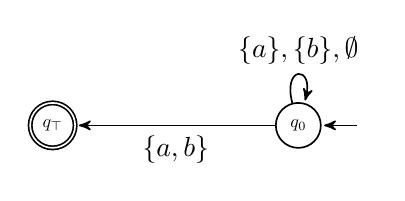
\begin{tikzpicture}[->,>=stealth',shorten >=1pt,auto,node distance=4.8cm,
                    semithick, initial text={}, initial where=right]
  \tikzstyle{every state}=[scale=0.65, every node/.style={scale=0.65}]

  \node[initial,state] (A)                {$\monstate_0$};
  \node[state, accepting]         (B) [left of  = A] {$\monstate_\top$};
 
  \path (A) edge              node {$ \{a,b\}$} (B)
     
            edge [loop above] node {$\{a\}, \{b\}, \emptyset$} (A) ;
\end{tikzpicture}    
\caption{$\monitor^\varphi$}
\end{subfigure} 

\hfill

\begin{subfigure} [b] {0.4\linewidth}
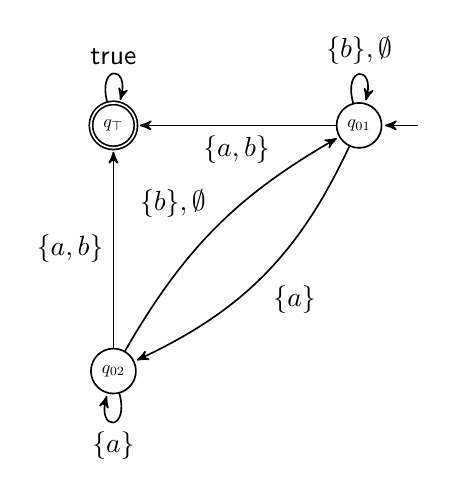
\begin{tikzpicture}[->,>=stealth',shorten >=1pt,auto,node distance=4.8cm,
                    semithick, initial text={}, initial where=right]
  \tikzstyle{every state}=[scale=0.65, every node/.style={scale=0.65}]

  \node[initial,state] (A)                {$\monstate_{01}$};
  \node[state, accepting]         (B) [left of  = A] {$\monstate_\top$};
  \node[state]         (D) [below of = B] {$\monstate_{02}$};

  \path (A) edge              node {$ \{a,b\}$} (B)
                 edge [loop above] node {$\{b\}, \emptyset$} (A)
                 edge      [bend left=20]     node   {$\{a\}$} (D)
        (B) edge [loop above] node {$\tru$} (B)
        (D) edge                 node {$\{a,b\}$} (B)
        (D) edge       [bend left=15]             node {$\{b\}, \emptyset$} (A)
        (D) edge [loop below] node {$\{a\}$} (D);

\end{tikzpicture}    
\caption{$\monitor_e^\varphi$}
\end{subfigure}
\caption{\LTLtri monitor vs. \Exltl~for $\varphi = \F (a \wedge b)$}
\label{fig:exltl-example}
\end{figure}


 

\ \   \ \


We have $\monitor^\varphi = \{ \{a, b\}, \{\monstate_0, \monstate_\top\}, 
\monstate_0, \delta, \lambda   \}$, where $\delta(\monstate_0, \{a\}) = 
\delta(\monstate_0, \{b\}) = \delta(\monstate_0, \emptyset) = \monstate_0$ and 
$\delta(\monstate_0, \{a, b\}) = \monstate_\top$. The set of outgoing 
transitions from monitor state $\monstate_0$ is $T_0 = \{t_0^0, t_\top^0\}$, 
where  $t_0^0 = \{\{a\}, \{b\}, \emptyset\}$ and $t_\top^0 = \{\{a,b\}\}$ are 
the outgoing transitions from monitor state $\monstate_0$ to monitor states 
$\monstate_0$ and $\monstate_\top$, respectively. We can verify that transition 
$t_0^0$ is \indist~from $t_\top^0$ since there is a state $\{a, b\} \in 
t_\top^0$ that is \covered~by transition $t_0^0$, i.e., $\dep (\{a, b\}, t_0^0) 
= \tru$. But $t_\top^0$ is not \indist~from $t_0^0$. Therefore, we have $N_0 = 
1$, $K_0 = 0$, $N_\top = 0$, and $K_\top = 0$. Since $N_0 > 0$, we \splt~$t_0^0$ 
into two transitions $t_{01}^0$ and $t_{02}^0$. Different \partitionn s of 
$t_0^0$ are as follows: 

\begin{tabbing}
\hspace{2cm}\= $t_{01}^{0,1} = \{\{a\}\}$ \hspace{1cm} \= $t_{02}^{0,1} = 
\{\{b\}, \emptyset\}$ \\
\> $t_{01}^{0,2} = \{\{b\}\}$ \> $t_{02}^{0,2} = \{\{a\}, \emptyset\}$ \\
\> $t_{01}^{0,3} = \{\emptyset\}$ \> $t_{02}^{0,3} = \{\{b\}, \{a\}\}$ 
\end{tabbing}

Note that there are $\frac{2^{|t_0^0|}-2}{2} = 3$ different \partitionn s. For 
each partition $t_{01}^{0,l}$ we calculate $N_{0l}$ and $K_{0l}$ as follows:


\begin{tabbing}
\hspace{2cm} \= $N_{01} = 0$ \hspace{1cm} \= $K_{01} = 0$ \\
\> $N_{02} = 0$ \> $K_{02} = 0$ \\
\> $N_{03} = 2$ \> $K_{03} = 1$
\end{tabbing}

We can verify that $\indisting(t_{02}^{0,3}, t_\top^0) = \tru$ and  
$\indisting(t_{02}^{0,3}, t_{01}^{0,3}) =\tru$, therefore $N_{03} = 2$. Also 
$\indisting(t_{02}^{0,3}, t_{01}^{0,3}) =\tru$ results in $K_{03} = 1$. As we 
can see partitions $\{t_{01}^{0,1}, t_{02}^{0,1}\}$ and $\{t_{01}^{0,2}, 
t_{02}^{0,2}\}$ are both optimum partitions as they result in minimal value for 
$N_{0l} + K_{0l}$. Thus, we \splt~$t_0^0$ into two transitions $t_{01}^0 = 
\{\{a\}\}$ and $t_{02}^0 = \{\{b\}, \emptyset\}$, and consequently add new 
monitor states $\monstate_{01}$ and $\monstate_{01}$ to $\monitor_e$ (see 
Figure \ref{fig:exltl-example}(b)). Since transition $t_0^0$ is a self-loop, 
therefore monitor state $\monstate_0$ is replaced by monitor state 
$\monstate_{01}$. The mapping function for the new monitor states is as follows:

\begin{center}
$\lambda(\monstate_{01}) = \lambda(\monstate_0) = ?$\\
$\lambda(\monstate_{02}) = \lambda(\monstate_0) = ?$
\end{center}

\noindent It is easy to verify that there are no more \indist~transitions in 
the monitor, therefore Figure \ref{fig:exltl-example} represents the final 
\Exltl~for $\varphi = \F (a \wedge b)$. 


\iffalse
\subparagraph{Example} We repeat the example from Section \ref{sec:SAMltl3} and 
this time we use \Exltl~in our algorithm.

$$\varphi = \F(a \wedge b)$$


Let $\monitor=\{M_1, M_2, M_3, M_4\}$, $s=\{a,b\}$, $S^s_1(a)=true$, 
$S^s_1(b)=\natural$, $S^s_2(a)=\natural$, $S^s_2(b)=true$, $S^s_3(a) =\natural$, 
$S^s_3(b) =\natural$,  $S^s_4(a) =\natural$, $S^s_4(b) =\natural$, and let 
$f=2$. According to Algorithm \ref{alg:localmonalgo3}, each local monitor $M_i$ 
computes an abstract local state $\abstate_i^1$ based on its concrete local 
state using abstraction functions $\mu_1$ and $\mu_2$ (cf. Line 
\fi


We now repeat the example from Section~\ref{sec:SAMltl3} for formula $\varphi = 
\F(a \wedge b)$ and this time we use \Exltl~in our algorithm (Algorithm 
\ref{alg:localmonalgo2}). Let $\monitor=\{M_1, M_2, M_3, M_4\}$, $s=\{a,b\}$, 
$S^s_1(a) = \tru$, $S^s_1(b)=\natural$, $S^s_2(a)=\natural$, $S^s_2(b)=\tru$, 
$S^s_3(a) =\natural$, $S^s_3(b) =\natural$,  $S^s_4(a) =\natural$, $S^s_4(b) 
=\natural$, and let $f=2$. According to Algorithm \ref{alg:localmonalgo2}, each 
local monitor $M_i$ computes an abstract local state $\abstate_i^1$ based on its 
concrete local state using abstraction functions $\mu_1$ and $\mu_2$ (cf. Line \ref{line:abst2}). Since all steps are as before except that we use \Exltl~in Algorithm \ref{alg:localmonalgo2}, we skip the details in order to avoid redundancy, and just recalculate the new verdict sets emitted by each local monitor (note that all local monitors are at the initial monitor state $\monstate_{01}$). 

Verdict sets after obtaining initial concrete local states: 

\begin{center}
$\pevent (\sample_1^\state) = \{\{a\}, \{a,b\}\} \; \Rightarrow \; \abstate_1^1 
= \verdict_1^1 =  \{\monstate_{02}, \monstate_\top\}$ 
$\pevent (\sample_2^\state) = \{\{b\}, \{a,b\}\} \; \Rightarrow \; \abstate_2^1 
= \verdict_2^1 =  \{\monstate_{01}, \monstate_\top\}$ 
$\pevent (\sample_3^\state) = \{\{a\}, \{b\}, \{a,b\}\} \; \Rightarrow \;
\abstate_3^1 = \verdict_3^1 =  \{\monstate_{01}, \monstate_{02}, 
\monstate_\top\}$ 
$\pevent (\sample_4^\state) = \{\{a\}, \{b\}, \{a,b\}\} \; \Rightarrow \;
\abstate_4^1 = \verdict_4^1 =  \{\monstate_{01}, \monstate_{02}, 
\monstate_\top\}$ 
\end{center}

At the end of round $1$: 

\begin{center}
$ \abstate_2^2 = \verdict_2^2 =  \{\monstate_\top\}$ \\
$ \abstate_3^2 = \verdict_3^2 =  \{\monstate_{01}, \monstate_\top\}$ \\
$ \abstate_4^2 = \verdict_4^2 =  \{\monstate_{01}, \monstate_\top\}$ 
\end{center}


At the end of round $2$: 

\begin{center} 
$ \abstate_3^3 = \verdict_3^3 =  \{\monstate_\top\}$ \\
$ \abstate_4^3 = \verdict_4^3 =  \{\monstate_{01}, \monstate_\top\}$ 
\end{center}



At the end of round $3$: 

\begin{center} 
$ \abstate_3^4 = \verdict_3^4 =  \{\monstate_\top\}$ \\
$ \abstate_4^4 = \verdict_4^4 =  \{\monstate_\top\}$ 
\end{center}


The following tables summarize the scenario:\\

\begin{tabular}{| c |c |c |c|}
\multicolumn{3}{c}{sample} \\
\hline
&$a$&$b$&$\abstate_i^1$\\
\hline
$M_1$ & $\tru$  & $\natural$ & $\{\monstate_{02}, \monstate_\top\}$\\
$M_2$ & $\natural$ & $\tru$ &  $\{\monstate_{01}, \monstate_\top\}$\\
$M_3$ & $\natural$ & $\natural$ &  $\{\monstate_{01},\monstate_{02}, 
\monstate_\top\}$ \\
$M_4$ & $\natural$ & $\natural$ &  $\{\monstate_{01}, \monstate_{02}, 
\monstate_\top\}$\\
%$M_5$ & $\natural$ & $true$ \\
\hline
\end{tabular} 
\quad
\begin{tabular}{| c |c|}
\multicolumn{2}{c}{round 1} \\
\hline
&$\abstate_i^2$\\
\hline
$M_1$ & crashed\\
$M_2$ & $\{\monstate_\top\}$\\
$M_3$ & $\{\monstate_{01}, \monstate_\top\}$ \\
$M_4$ & $\{\monstate_{01}, \monstate_\top\}$ \\
%$M_5$ & $\natural$ & $true$ \\
\hline
\end{tabular}
\quad
\begin{tabular}{| c |c|}
\multicolumn{2}{c}{round 2} \\
\hline
&$\abstate_i^3$\\
\hline
$M_1$ & crashed\\
$M_2$ & crashed\\
$M_3$ & $\{\monstate_\top\}$ \\
$M_4$ & $\{\monstate_{01}, \monstate_\top\}$ \\
%$M_5$ & $\natural$ & $true$ \\
\hline
\end{tabular} 

\begin{tabular}{| c |c|}
\multicolumn{2}{c}{round 3} \\
\hline
&$\abstate_i^4$\\
\hline
$M_1$ & crashed\\
$M_2$ & crashed\\
$M_3$ & $\{\monstate_\top\}$ \\
$M_4$ & $\{\monstate_\top\}$ \\
%$M_5$ & $\natural$ & $true$ \\
\hline
\end{tabular} \\ \\



\noindent As we observe, at the end of round $3$ (namely, $f+1$), the abstract 
local states of all nonfaulty monitors include the single monitor state 
$\monstate_\top$, and therefore they both emit the same 
\truthvalue~$\lambda(\monstate_\top) = \top$.



\subsubsection{Proof of Correctness of Algorithm \ref{alg:localmonalgo2}}

%\todo{What do you mean by completeness here? You only have to prove the 
%requirement of your problem statement which is essentially soundness.}

In order to prove the soundness of Algorithm \ref{alg:localmonalgo2}, we have to 
prove that $|\mathcal{I}^{\monstate}| =1$ at every monitor state $\monstate \in 
Q_e$. As described above, an \Exltl~is constructed such that at every monitor 
state $\monstate \in Q_e$, every two outgoing transitions $t_j^\monstate$ and 
$t_k^\monstate$ from monitor state $\monstate$ are \dist. Therefore, to prove 
the soundness of Algorithm \ref{alg:localmonalgo2}, it suffices to prove the following theorem.



\begin{theorem}
\label{theorem:soundness}
 If at every monitor state $\monstate \in Q_e$, every two outgoing transitions 
$t_j^\monstate$ and $t_k^\monstate$ from monitor state $\monstate$ are \dist, 
then we have $|\intersection| =1$. Formally
$$(\forall t_j^\monstate , t_k^\monstate \in T_\monstate .~ \disting(t_j^\monstate , t_k^\monstate)) \Leftrightarrow |\intersection| =1$$ where $T_\monstate$ is the set of all outgoing transitions from monitor state $\monstate$.

\end{theorem} 

We prove theorem \ref{theorem:soundness} in two steps. First, we prove that

$$(\forall t_j^\monstate , t_k^\monstate \in T_\monstate .~ \disting(t_j^\monstate , t_k^\monstate)) \Rightarrow |\intersection| =1$$

Proof is by contradiction. Suppose every transition in $T_i$ is \indist~from all other transitions in $T_i$, and suppose $|\intersection| > 1$. Let $\state$ be the global state of the system and suppose $\delta(\monstate, \state) = \monstate_k$, therefore we know $\monstate_k \in \intersection$. Since $|\intersection| > 1$, thus there exists another monitor state $\monstate_j \in \intersection$. Since $\monstate_j \in \intersection$ therefore for every local monitor $M_i$ there exists an state $\state' \in t_j^\monstate$ that is possible to be the global state. We also assumed that the set of monitors satisfy the state coverage, thus for every $\ap \in \AP$, there exists monitor $M_i$ such that $\sample_i^\state(\ap) \neq \udef$. Formally:


\begin{enumerate}
\item $\forall \ap \in \AP. ~ \exists M_i \in \monitor.~ (\sample_i^{\state'}(ap) = \tru \rightarrow ap \in \state) \wedge  (\sample_i^{\state'}(ap) = \fals \rightarrow ap \notin \state) )$
\item $\forall M_i \in \monitor.~ \exists \state' \in t_j^q.~ \state' \in \pevent_i$
\end{enumerate}


Therefore, for every $\ap \in \AP$ there exists $\state' \in t_j^\monstate$ such that $(\ap \in \state' \Leftrightarrow \ap \in \state)$, which means that $\state$ is \covered~by $t_j^\monstate$, and consequently $t_j^\monstate$ is \indist~from $t_k^\monstate$, which is a contadiction, hence the proof is complete.



Now we have to prove that

$$  |\intersection| =1   \Rightarrow  (\forall t_j^\monstate , t_k^\monstate \in T_\monstate .~ \disting(t_j^\monstate , t_k^\monstate))$$

The proof, again, is by contradiction. Suppose $|\intersection| = 1$ and suppose there exist transitions $t_j^\monstate$ and $t_k^\monstate$ such that $\indisting(t_j^\monstate, t_k^\monstate) = \tru$. According to Definition \ref{def:indisting}, transition $t_j^\monstate$ 
is \indist~from $t_k^\monstate$ if there exists an state $\state' \in t_k^\monstate$ 
such that $\state'$ is \covered~by $t_j^\monstate$, i.e.,
$$ \forall \ap \in \AP.~ \exists \state \in t_j^\monstate. ~(\ap \in \state' \Leftrightarrow \ap \in \state) $$

Now consider the case where the global state of the system under inspection is $\state'$ and let us verify how the local monitors emit their verdicts. Recall from Section \ref{sec:SAMltl3}, that $\intersection$ is the intersection of all verdict sets emitted by the local monitors which have partial view (concrete local state) of the global state of the system, such that their concrete local states satisfy the state coverage (see Definition \ref{def:state coverage}). It is easy to verify that the worst case scenario, upon which an \Exltl~is constructed, is when each verdict set is emitted by a monitor which knows the value of at most one atomic proposition $\ap \in \AP$. Consider the global state $\state'$, since $\state' \in t_k^\monstate$ thus we have $\delta(\monstate, \state') = \monstate_k$, where $\monstate_k$ is the monitor state for which $t_k^\monstate$ is an incoming transition.  Therefore a local monitor $M_i$ which has full view of the state $\state'$, i.e., for every $\ap \in \AP$, $\sample_i^{\state'}(\ap) \neq \natural$, emits the verdict $\{\monstate_k\}$. However, in the worst case scenario, each local monitor only reads the value of one atomic proposition. In this case, we can verify that

 $$\forall i \in [1, n].~ \monstate_j \in \verdict_i^1$$ where $\verdict_i^1$ is the verdict set emitted by monitor $M_i$ at round $1$ (recall from Algorithm \ref{alg:localmonalgo2} that $\verdict_i^1$ is calculated based on $M_i$'s concrete local state), and $\monstate_j$ is the monitor state for which $t_j^\monstate$ is an incoming transition. This holds because we have 

$$ \forall \ap \in \AP.~ \exists \state \in t_j^\monstate. ~(\ap \in \state' \Leftrightarrow \ap \in \state) $$

To see this more clearly, we need to recall the definition of the set of possible \events~$\pevent_i$ from viewpoint of a local monitor $M_i$,

\begin{center}
$\pevent(\sample_i^{\state'}) = \{ \state \in \alphabet ~|~ \forall ap \in \AP: (\sample_i^{\state'}(ap) \neq \natural) \rightarrow ( (\sample_i^{\state'}(ap) = \tru \rightarrow ap \in \state) \wedge  (\sample_i^{\state'}(ap) = \fals \rightarrow ap \notin \state) ) \} $
\end{center}

Now all we need to do is to show that

$$\forall i \in [1, n].~ \exists \state \in t_j^\monstate . ~ \state \in \pevent_i$$
 
and consequently, $\monstate_j \in \verdict_i^1$ for every $i \in [1, n]$.




In order to prove the above statement we claim that
$$ \nexists \ap \in \AP.~  (  \sample_i^{\state'} (\ap) \neq \natural )  \wedge (\nexists \state \in t_j^\monstate.~ (\ap \in \state' \Leftrightarrow \ap \in \state) ) $$ 


Informally, for every local monitor $M_i$, there is an atomic proposition $\ap \in \AP$ such that $\sample_i^{\state'} = \natural$ (since we assumed no local monitor has the full view of the system), and there exists \event~$\state \in t_j^\monstate$ such that $(\ap \in \state' \Leftrightarrow \ap \in \state)$ (since $\state'$ is \covered~by $t_j^\monstate$). Therefore according to definition of $\pevent_i$, we have $\state \in \pevent_i$, and hence $\monstate_j \in \verdict_i^1$. Thus we proved that 


$$ \indisting(t_j^\monstate, t_k^\monstate) \Rightarrow \exists \state \in t_k^\monstate. ~  \forall i \in [1, n].~ \{ (\exists \ap \in \AP.~ \sample_i^\state(\ap) = \natural ) \rightarrow  \monstate_j \in \verdict_i^1\}$$
 
Therefore in the worst case scenario where no local monitor has the full view of the system, $\monstate_j$ will appear in the verdict set emitted by each monitor, and therefore $|\intersection| > 1$, which is a contradiction, and the proof is complete.


Algorithm \ref{alg:extendedmonalg} constructs an \Exltl~$\monitor_e^\varphi$ such that at every monitor state $\monstate \in Q_e$, every outgoing transition is \dist~from all other outgoing transitions, and therefore $|\intersection| = 1$ at every $\monstate \in Q_e$. 


\iffalse

\subsubsection{Complexity of Algorithm \ref{alg:extendedmonalg}}


Consider Algorithm \ref{alg:extendedmonalg}: given \LTLtri monitor $\monitor^\varphi$, the number of outgoing transitions from each monitor state $\monstate_i \in Q$ is $2^{|\AP|}$ in the worst case, i.e., $|T_i| \leqslant 2^{|\AP|}$ . For every two outgoing transitions $t_j^i$ and $t_k^i$, the algorithm checks whether $\indisting(t_j^i, t_k^i)$ and $\indisting(t_k^i, t_j^i)$ (cf. Lines \ref{line:indisting}-\ref{line:indistingend}), each of which costs $|AP|.|t_j^i|.|t_k^i|$. We should note that $|t_1^i| + |t_2^i| + \cdots + |t_{m_\monstate}^i| = |T_i|$. Therefore it is easy to verify that the total cost to prerform Lines \ref{line:indisting}-\ref{line:indistingend} is $O(2^{2^{|\AP|}})$. It also causes an exponential blow-up in time with respect to $|t_j^i|$ to split $t_j^i$ (cf. Lines \ref{line:split0}-\ref{line:lambda-update1}), as $\frac{2^{| t_j^i|}-2}{2}$ partitions are generated by function \partition. In total, Algorithm \ref{alg:extendedmonalg} will cost double exponential time with respect to $|\AP|$, i.e., $O(2^{2^{|\AP|}})$. In online monitoring since the monitor is generated only once, the complexity for monitor construction is usually negligible. However, the complexity of the monitor for checking an execution (e.g., Algorithm \ref{alg:localmonalgo2}) are of important interest, since the monitor is part of the running system and should cause a minimal loss on the response time of the system.

\fi




          
         % \setcounter{figure}{0}
       % \setcounter{equation}{0}
       % \setcounter{table}{0}


 \chapter{Decentralized Asynchronous Monitoring}
\label{chap:DAM}






This Chapter discusses the decentralized asynchronous monitoring problem in the presence of faulty monitors. The problem statement and the challenges in asynchronous monitoring are discussed in Sections \ref{sec:PSa} and \ref{sec:challenge-as}, respectively. Model of computation and terminology are presented in Section \ref{sec:model-as}. In Section \ref{sec:AMAltl3} we propose an automata-based algorithm which employs \LTLtri monitor to compute the verdict sets emitted by local monitors. Finally in Section \ref{sec:AMAExltl} we present an Algorithm that uses an \Exltl~to solve the decentralized asynchronous monitoring problem where local monitors emit their verdicts without any round of communication (i.e., accessing the shared memory).




\iffalse
We present an algorithm for asynchronous distributed fault-tolerant RV, where the monitors are asynchronous wait-free processes that any of them can fail by crashing. Similar to our synchronous model (Section \ref{sec:DSM}), each local monitor obtains a partial view (i.e., a concrete local state) of the system's global state. It communicates with other monitors through a shared memory and updates its knowledge, and then solely based on its partial view, emits a final verdict. We show how, given any \LTL formula and an \Exltl, a set of verdicts collectively provided by the local monitors can be used to compute the verdict computed by a centralized monitor that has full view of the system under scrutiny.
\fi



\section{Problem Statement}
\label{sec:PSa}

The system under inspection produces a finite trace $\alpha = \state_0 \state_1 \cdots \state_k$, and is inspected with respect to an \LTL formula $\varphi$ by a set $\monitor = \{ M_1, M_2, \cdots , M_n \}$ of asynchronous distributed wait-free monitors. The notion of wait-free distributed monitoring is formally introduced in \cite{bfrrt16} as follows.


\begin{definition}
\label{def:wait-free}
By wait-free monitoring we mean that each monitor (1) runs at its own speed, that may vary along with time and (2) may fail by crashing (i.e., halt and never recover), thus a monitor never “waits” for another monitor (in order to avoid a livelock).
\end{definition}


For every $j \in [0, k-1]$, between each $\state_j$ and $\state_j+1$, each monitor $M_i \in \monitor$, $i \in 
[1, n]$, in a wait-free manner: \\ 1. reads the value of propositions in $\state_j$, which may result in a partial observation of $\state_j$;\\
2. repeatedly communicates its partial observation with other monitors through a single-writer/multi-reader shared memory; \\
3. updates its knowledge resulting from the aforementioned communication, and \\
4. evaluates $\varphi$ and emits a verdict based on its current knowledge. \\


% !TEX root = main.tex
\begin{algorithm}[H]
\small
\KwData{\LTL formula $\varphi$ and state $\state_j$}
\KwResult{a verdict from $\mathbb{B}_3$}
%$j = 0$\;
%\While{\rm there is a new state $s_j$}{
Let $\sample_i^{s_j}$ be the initial concrete local state of the monitor    \;  \label{line:init4}
$\LS_i^{\state_j} \gets$ $\sample_i^{s_j}$\tcc*[r]{\it take sample from state $s_j$}
\label{line:sample4} 
\For{\rm some fixed number of rounds $r \geqslant 1$}{
$\SM_i^{\state_j} \gets \pred(\LS_i^{\state_j})$\tcc*[r]{\it write current knowledge in shared memory} \label{line:write4} 
$\LS_i^{\state_j} \gets$ $\SM^{\state_j}$\tcc*[r]{\it take a snapshot of the shared memory}
} \label{line:snapshot4}
emit {$[\extr(\LS_i^{\state_j})\dots\extr(\LS_i^{\state_j})\models_4 
\varphi$}]\tcc*[r]{\it evaluate $\varphi$ using extrapolation function} 
%\label{line:emit}
%$j \gets j + 1$\;}
\caption{Behavior of Monitor $M_i$, for $i\in [1, n]$}
\label{alg:localmonalgo4}
 \end{algorithm}

 \ \



Each monitor $M_i$ in $\monitor$ is a process, and the monitors run in the standard asynchronous wait-free read/write shared memory model \cite{aw04}. We assume that up to $n-1$ monitors can crash. Every monitor that does not fail is required to emit a verdict. Hence, a distributed algorithm in this settings consists for each monitor in a bounded sequence of read/write accesses to the shared memory at the end of which a verdict is emitted. We thus assume without loss of generality that each monitor may access the shared memory a fixed number of times before emitting a verdict \cite{hkr13, bfrrt16}. 

In our setting the assumption is that the set of monitors satisfy the state coverage. Thus if a proposition is read by only one monitor, then this monitor is supposed to send its information to at least one nonfaulty monitor before crashing. 

Algorithm \ref{alg:localmonalgo4} represents the aforementioned asynchronous monitoring scenario. Our problem statement is that when a non-faulty monitor runs Algorithm~\ref{alg:localmonalgo4}, it should compute and emit a verdict such that it ensures consistent distributed monitoring. Namely, one has to be able to map a collective set of verdicts of monitors (for any execution interleaving) to one and only one verdict of a centralized monitor that has the full view $\state_j$. A necessary condition for this mapping is that, for every two finite traces  $\alpha, \alpha' \in \alphabet^\ast$, if $[\alpha \models_3 \varphi] \neq [\alpha' \models_3 \varphi] $ (or alternatively, $[\alpha \models_4 \varphi] \neq [\alpha' \models_4 \varphi] $), then the monitors in $\monitor$ should compute different collective sets of verdicts for $\alpha$ and $\alpha'$, regardless of their initial partial observation and different read/write interleavings.


\section{Model of Computation and Terminology}
\label{sec:model-as}
For every state $\state_j$ in $\alpha = \state_0 \state_1 \cdots \state_k$, each monitor $M_i$ maintains a \localreg~$\LS_i$. Each \localreg~has $n$ registers, one per each monitor in $\monitor$. The local register of monitor $M_i$ associated with monitor $M_l$ for state $\state_j$ is denoted by $\LS_i^{\state_j}[l]$. Each register has $|AP|$ elements, one for each atomic proposition in $AP$. The monitors in $\monitor$ communicate by means of shared memory. The structure of the shared memory $\SM$ is as follows: for each state $\state_j$, $\SM^{\state_j}$ consists of $n$ atomic registers, one per monitor, and each register has $|AP|$ elements one for each atomic proposition (i.e, single-writer/multiple-reader (SWMR) registers). Thus, for state $\state_j$, each monitor $M_i$ can read the entire content of $\SM^{\state_j}$, but can only write into register $\SM_i^{\state_j}$. We assume that each monitor is aware of the change of state of the system under inspection. Thus, for a state $\state_j$, a monitor $M_i$ reads and writes in the associated local and shared memory locations, i.e., $\LS_i^{\state_j}$ and $\SM^{\state_j}$. \\ 


\subparagraph{The asynchronous monitoring algorithm.}  Each monitor $M_i \in \monitor$ , $i \in [1, n]$, runs Algorithm \ref{alg:localmonalgo4}. For any given new state $\state_j$, Monitor $M_i$ first initializes all elements of its \localreg~to $\natural$ (cf. Line \ref{line:init4}). Then, $M_i$ takes a sample from state $\state_j$ and obtains a concrete local state $\sample_i^{\state_j}$(cf. Line \ref{line:sample4}). Recall from Definition \ref{def:concretestate} that the value of an atomic proposition in a concrete local state is either $\tru$, $\fals$, or $\natural$. We assume that the set of monitors satisfy the state coverage whose definiton was presented in Chapter \ref{chap:extended monitor}. The set of values in the concrete local state is copied in \localreg~$\LS_i^{\state_j}$. Then each monitor $M_i$ executes a sequence of write/read actions (cf. Lines \ref{line:write4} and \ref{line:snapshot4}) for some a priori known number of times. in Line  \ref{line:write4}, it atomically writes the content of its \localreg~$\LS_i^{\state_j}$ into its associated register $\SM_i^{\state_j}$ in the shared memory. In Line \ref{line:snapshot4}, $M_i$ reads of all the registers in $\SM_i^{\state_j}$, and copies them into $\LS_i^{\state_j}$, in a single atomic step.



\section{Challenges in Asynchronous Monitoring}
\label{sec:challenge-as}


In \cite{bfrrt16} it is shown that \RVLTL is not sufficient to consistenly monitor the global system state in a distributed asynchronous environment. To overcome this insufficiency, they introduced a family of multi-valued logics (called \LTLk), for every $k \geqslant 0$, where $k$ relates to the notion of alternation number which is introduced and formally defined in \cite{bfrrt16}.  

We use the example from \cite{bfrrt16} and we show how each local monitor runs Algorithm \ref{alg:localmonalgo4} and emits a verdict from $\mathbb{B}_4$ based on the final content of its \localreg. \\





\subparagraph{Example}
Let $\monitor = \{M_1, M_2\}$ and consider the formula for two requests and  
acknowledgments: 
\[
\varphi_{ra_2} = \Big(\G(\neg a_1 \wedge \neg r_1) \, \vee \, [(\neg a_1 \, 
\U \, r_1) \, \wedge \, \F a_1]\Big)\, \wedge \, \Big(\G(\neg a_2 \wedge \neg 
r_2) \, \vee \, [(\neg a_2 \, \U \, r_2) \,\wedge \, \F a_2]\Big)
\]
Fig.~\ref{fig:example1} shows different execution interleavings of monitors 
$M_1$ and $M_2$ when running Algorithm~\ref{alg:localmonalgo} from states 
$\state_0  = \{r_1, a_1\}$ and $\state_0' = \{r_1, a_1, r_2\}$. Based on the 
order of monitor write-snapshot actions: $M_1, M_2$ (resp., $M_2, M_1$) denotes 
the case where monitor $M_1$ (resp., $M_2$) executes a write-snapshot before 
monitor $M_2$ (resp., $M_1$) does, and $M_1|| M_2$ denotes the case where 
monitors $M_1$ and $M_2$ execute their write-snapshot actions concurrently. In 
case of $\state_0$, after executing Line~\ref{line:sample4} of 
Algorithm~\ref{alg:localmonalgo4}, monitor $M_1$'s sample, i.e., the local 
snapshot $\LS_1^{\state_0}[1]$, consists of $\sample_1^{\state_0}(r_1) = \tru$,  
$\sample_1^{\state_0}(a_1) = \udef$, and $\sample_1^{\state_0}(r_2) = 
\sample_1^{\state_0}(a_2) = \fals$. Moreover, initially, $M_1$ has no knowledge 
of $M_2$'s sample. Monitor $M_2$'s sample from $\state_0$, i.e., the local 
snapshot $\LS_2^{\state_0}[2]$, consists of $\sample_2^{\state_0}(r_1) = 
\sample_2^{\state_0}(a_1) = \tru$, $\sample_2^{\state_0}(r_2)=\udef$, and 
$\sample_2^{\state_0}(a_2)= \fals$ while it initially has no knowledge of 
$M_1$'s sample. Likewise, for state $\state'_0$, Fig.~\ref{fig:example1} 
shows different local snapshots by $M_1$ and $M_2$. Given two values $v_1$ and 
$v_2$, we define (an arbitrary) extrapolation function as follows:
\begin{equation*}
%\label{eq:fra}
\extr_\ap(v_1, v_2) = \begin{cases}
\tru   & \mbox{if } (v_1=\tru)  \, \vee \, (v_2=\tru) \\
\fals & \mbox{otherwise} \end{cases} 
\end{equation*}
where $\ap \in \{a_1, r_1, a_2, r_2\}$.
% The intuition behind this is that if some monitor observes a request, say 
% $r_1$, (respectively, an acknowledgment, say $a_1$), then this 
% request (respectively, acknowledgment) exists; i.e., $r_1 = \tru$ 
% (respectively, $a_1 = \tru$). Otherwise, the request (respectively,
% acknowledgment) does not exist; i.e $r_1 = \fals$ (respectively, $a_1 = 
% \fals$).
Finally, starting from $\state_0$, if (1) the for loop of 
Algorithm~\ref{alg:localmonalgo4} terminates after 1~communication round, and 
(2) the interleaving is $M_1, M_2$, then $\extr(\llbracket \LS_2^{\state_0} \rrbracket) 
= \{r_1, a_1\}$, and  evaluation of $\varphi_{ra_2}$ by $M_2$ in \LTLfour 
results in $[\extr(\llbracket \LS_2^{\state_0} \rrbracket) \models_4 \varphi_{ra_2}] = 
\top_p$. 

%%%%%%%%%%%%%%%%%%%%%%%%%%%%%%%%%%%%%%%%%%%%%%%%
% EXAMPLE 
% !TEX root = main.tex
\begin{figure}[H]
\hspace{-8mm}
\scriptsize
\tiny
\begin{minipage}{\textwidth}
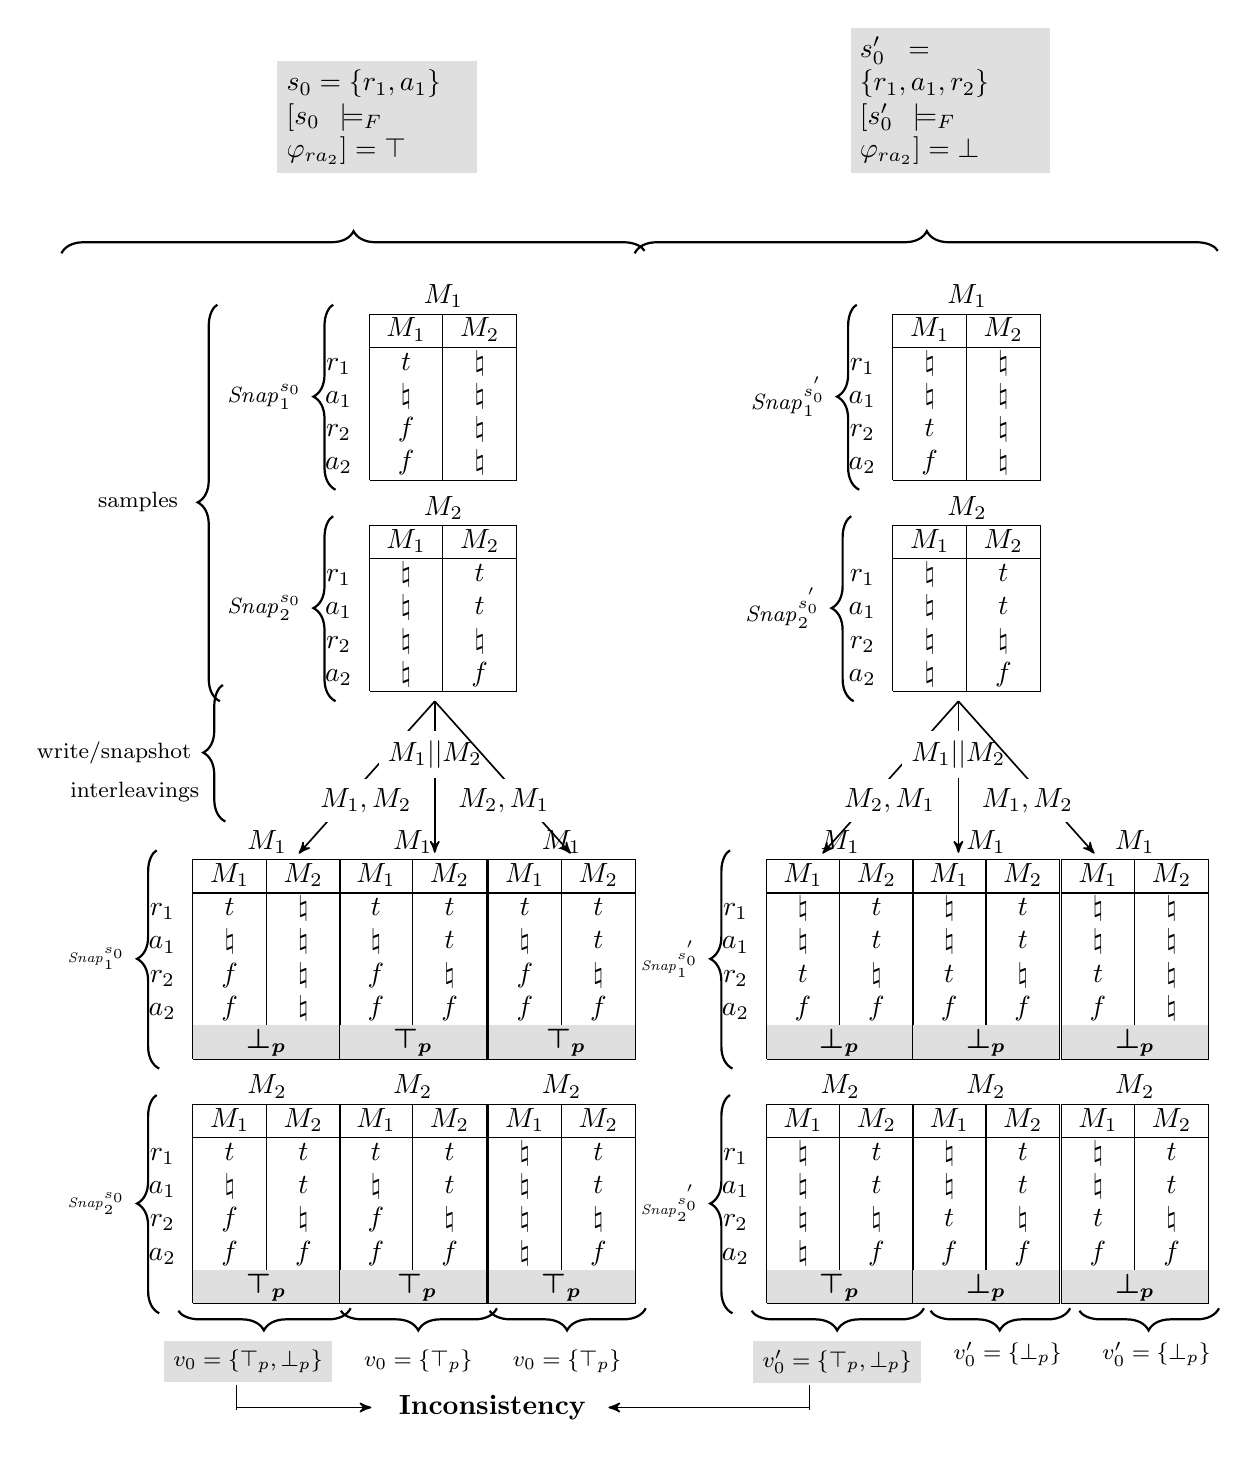
\begin{tikzpicture}[->,>=stealth',shorten >=1pt,auto,node distance=2.8cm,
                    semithick, initial text={}, initial where=right, scale=.7]
                    
\begin{scope}
\node (tab1) {
  \begin{tabular}{c|c|c|}
   \multicolumn{1}{r}{} &  \multicolumn{2}{c}{ {$M_1$}}\\
  \cline{2-3}
  & $M_1$ & $M_2$\\
  \cline{2-3}
   $r_1$ & $t$ & $\udef$\\
   $a_1$ & $\udef$ & $\udef$\\
   $r_2$ & $f$ & $\udef$\\
   $a_2$ & $f$ & $\udef$\\
   \cline{2-3}
  \end{tabular}
};

\node [below = -1mm of tab1] (tab2) {
\begin{tabular}{c|c|c|}
    \multicolumn{1}{r}{} &  \multicolumn{2}{c}{ {$M_2$}}\\
  \cline{2-3}
  & $M_1$ & $M_2$\\
  \cline{2-3}
   $r_1$ & $\udef$ & $t$\\
   $a_1$ & $\udef$ & $t$\\
   $r_2$ & $\udef$ & $\udef$\\
   $a_2$ & $\udef$ & $f$\\
   \cline{2-3}
  \end{tabular}
};

\end{scope}

\draw[-] [decorate,decoration={brace,amplitude=8pt},decorate, thick]
([xshift=-1.4cm]tab1.south) -- ([xshift=-1.4cm, yshift=-6mm]tab1.north) node 
[black,midway,xshift=-0.3cm] {\footnotesize $\LS_1^{\state_0}$};

\draw[-] [decorate,decoration={brace,amplitude=8pt},decorate, thick]
([xshift=-1.4cm]tab2.south) -- ([xshift=-1.4cm, yshift=-6mm]tab2.north) node 
[black,midway,xshift=-0.3cm] {\footnotesize $\LS_2^{\state_0}$};

\draw[-] [decorate,decoration={brace,amplitude=8pt},decorate, thick]
([xshift=-3.5cm]tab2.south) -- ([xshift=-3.5cm, yshift=-6mm]tab1.north) node 
[black,midway,xshift=-0.4cm] {\footnotesize 
samples};

\begin{scope}[xshift=-3.2cm, yshift=-10.2cm]
\node (tab3) {
  \begin{tabular}{c|c|c|}
   \multicolumn{1}{r}{} &  \multicolumn{2}{c}{ {$M_1$}}\\
  \cline{2-3}
  & $M_1$ & $M_2$\\
  \cline{2-3}
   $r_1$ & $t$ & $\udef$\\
   $a_1$ & $\udef$ & $\udef$\\
   $r_2$ & $f$ & $\udef$\\
   $a_2$ & $f$ & $\udef$\\
   \cline{2-3}
    &  \multicolumn{2}{c|}{\cellcolor{gray!25}$\boldsymbol{\bot_p}$}\\
   \cline{2-3}
  \end{tabular}
};
\node [below = -1mm of tab3] (tab4) {
\begin{tabular}{c|c|c|}
    \multicolumn{1}{r}{} &  \multicolumn{2}{c}{ {$M_2$}}\\
  \cline{2-3}
  & $M_1$ & $M_2$\\
  \cline{2-3}
   $r_1$ & $t$ & $t$\\
   $a_1$ & $\udef$ & $t$\\
   $r_2$ & $f$ & $\udef$\\
   $a_2$ & $f$ & $f$\\
   \cline{2-3}
   &  \multicolumn{2}{c|}{\cellcolor{gray!25}$\boldsymbol{\top_p}$}\\
   \cline{2-3}
  \end{tabular}
};
\end{scope}

\begin{scope}[yshift=-10.2cm] \node (tab5) {
  \begin{tabular}{|c|c|}
   \multicolumn{2}{c}{ {$M_1$}}\\
  \cline{1-2}
   $M_1$ & $M_2$\\
  \cline{1-2}
   $t$ & $t$\\
   $\udef$ & $t$\\
   $f$ & $\udef$\\
   $f$ & $f$\\
   \cline{1-2}
   \multicolumn{2}{|c|}{\cellcolor{gray!25}$\boldsymbol{\top_p}$}\\
   \cline{1-2}
  \end{tabular}
};
\node [below = -1mm of tab5] (tab6) {
\begin{tabular}{|c|c|}
  \multicolumn{2}{c}{ {$M_2$}}\\
  \cline{1-2}
   $M_1$ & $M_2$\\
  \cline{1-2}
   $t$ & $t$\\
   $\udef$ & $t$\\
   $f$ & $\udef$\\
   $f$ & $f$\\
   \cline{1-2}
   \multicolumn{2}{|c|}{\cellcolor{gray!25} $\boldsymbol{\top_p}$}\\
   \cline{1-2}
  \end{tabular}
};
\end{scope}

\begin{scope}[xshift=2.7cm, yshift=-10.2cm]
\node (tab7) {
  \begin{tabular}{|c|c|}
   \multicolumn{2}{c}{ {$M_1$}}\\
  \cline{1-2}
  $M_1$ & $M_2$\\
  \cline{1-2}
   $t$ & $t$\\
   $\udef$ & $t$\\
   $f$ & $\udef$\\
   $f$ & $f$\\
   \cline{1-2}
   \multicolumn{2}{|c|}{\cellcolor{gray!25} $\boldsymbol{\top_p}$}\\
   \cline{1-2}
  \end{tabular}
};
\node [below = -1mm of tab7] (tab8) {
\begin{tabular}{|c|c|}
    \multicolumn{2}{c}{ {$M_2$}}\\
  \cline{1-2}
   $M_1$ & $M_2$\\
  \cline{1-2}
   $\udef$ & $t$\\
   $\udef$ & $t$\\
   $\udef$ & $\udef$\\
   $\udef$ & $f$\\
   \cline{1-2}
   \multicolumn{2}{|c|}{\cellcolor{gray!25}$\boldsymbol{\top_p}$}\\
   \cline{1-2}
  \end{tabular}
};
\end{scope}


\draw[-] [decorate,decoration={brace,amplitude=8pt},decorate, thick]
([xshift=-1.1cm, yshift=12.5cm]tab3.west) -- ([yshift=12.5cm]tab7.east) 
node [black,midway, yshift=1cm, text width=2.3cm,xshift=3mm,fill=gray!25] 
{$\state_0 = \{r_1, a_1\}$ \\ $[\state_0 \models_F \varphi_{ra_2}] = \top$ };




\draw[-] [decorate,decoration={brace,amplitude=8pt},decorate, thick]
([xshift=-.2cm, yshift=-1mm]tab3.north) -- ([xshift=-.2cm, 
yshift=24mm]tab3.north) node [black,midway,xshift=-0.3cm] {\footnotesize 
write/snapshot} node [black,midway,yshift = -5mm, xshift=-.2cm] {\footnotesize 
interleavings};


\draw[->] ([xshift=.4cm]tab2.south) -- +(-2.5, -2.8) 
node[draw=none,fill=white,midway,left, below] {$M_1, M_2$};

\draw[->] ([xshift=.4cm]tab2.south) -- +(0, -2.8) node 
[draw=none,fill=white,midway, above] {$M_1||M_2$};
  
\draw[->] ([xshift=.4cm]tab2.south) -- +(2.5, -2.8) 
node[draw=none,fill=white,midway,below] {$M_2, M_1$};

\draw[-] [decorate,decoration={brace,amplitude=8pt},decorate, thick]
([xshift=-1.4cm]tab3.south) -- ([xshift=-1.4cm, yshift=-6mm]tab3.north) node 
[black,midway,xshift=-0.3cm] {\tiny $\LS_1^{\state_0}$};

\draw[-] [decorate,decoration={brace,amplitude=8pt},decorate, thick]
([xshift=-1.4cm]tab4.south) -- ([xshift=-1.4cm, yshift=-6mm]tab4.north) node 
[black,midway,xshift=-0.3cm] {\tiny $\LS_2^{\state_0}$};

\draw[-] [decorate,decoration={brace,amplitude=8pt},decorate, thick]
([yshift=-2.2cm]tab4.east) -- ([xshift=10mm,yshift=-2.2cm]tab4.west) node 
[black,midway,yshift=-0.4cm,xshift=-2mm,fill=gray!25] {\footnotesize 
$v_0=\{\top_p, \bot_p\}$};

\draw[-] [decorate,decoration={brace,amplitude=8pt},decorate, thick]
([yshift=-2.2cm]tab6.east) -- ([xshift=2mm,yshift=-2.2cm]tab6.west) node 
[black,midway,yshift=-0.4cm] {\footnotesize $v_0=\{\top_p\}$};

\draw[-] [decorate,decoration={brace,amplitude=8pt},decorate, thick]
([yshift=-2.2cm]tab8.east) -- ([xshift=2mm,yshift=-2.2cm]tab8.west) node 
[black,midway,yshift=-0.4cm] {\footnotesize $v_0=\{\top_p\}$};

%----------------------------s'_0 State---------------------------------

\begin{scope}[xshift=9.5cm] \node (tabb1) {
  \begin{tabular}{c|c|c|}
   \multicolumn{1}{r}{} &  \multicolumn{2}{c}{ {$M_1$}}\\
  \cline{2-3}
  & $M_1$ & $M_2$\\
  \cline{2-3}
   $r_1$ & $\udef$ & $\udef$\\
   $a_1$ & $\udef$ & $\udef$\\
   $r_2$ & $t$ & $\udef$\\
   $a_2$ & $f$ & $\udef$\\
   \cline{2-3}
  \end{tabular}
};
\node [below = -1mm of tabb1] (tabb2) {
\begin{tabular}{c|c|c|}
    \multicolumn{1}{r}{} &  \multicolumn{2}{c}{ {$M_2$}}\\
  \cline{2-3}
  & $M_1$ & $M_2$\\
  \cline{2-3}
   $r_1$ & $\udef$ & $t$\\
   $a_1$ & $\udef$ & $t$\\
   $r_2$ & $\udef$ & $\udef$\\
   $a_2$ & $\udef$ & $f$\\
   \cline{2-3}
  \end{tabular}
};
\end{scope}


\draw[-] [decorate,decoration={brace,amplitude=8pt},decorate, thick]
([xshift=-1.4cm]tabb1.south) -- ([xshift=-1.4cm, yshift=-6mm]tabb1.north) node 
[black,midway,xshift=-0.3cm] {\footnotesize $\LS_1^{\state^{'}_0}$};

\draw[-] [decorate,decoration={brace,amplitude=8pt},decorate, thick]
([xshift=-1.5cm]tabb2.south) -- ([xshift=-1.5cm, yshift=-6mm]tabb2.north) node 
[black,midway,xshift=-0.3cm] {\footnotesize $\LS_2^{\state^{'}_0}$};

\draw[->] ([xshift=.4cm]tabb2.south) -- +(-2.5, -2.8) 
node[draw=none,fill=white,midway,below] {$M_2, M_1$};

\draw[->] ([xshift=.4cm]tabb2.south) -- +(0, -2.8) node 
[draw=none,fill=white,midway, above] {$M_1||M_2$};
  
\draw[->] ([xshift=.4cm]tabb2.south) -- +(2.5, -2.8) 
node[draw=none,fill=white,midway,below] {$M_1, M_2$};


\begin{scope}[xshift=7.2cm, yshift=-10.2cm]
\node (tabb3) {
  \begin{tabular}{c|c|c|}
   \multicolumn{1}{r}{} &  \multicolumn{2}{c}{ {$M_1$}}\\
  \cline{2-3}
  & $M_1$ & $M_2$\\
  \cline{2-3}
   $r_1$ & $\udef$ & $t$\\
   $a_1$ & $\udef$ & $t$\\
   $r_2$ & $t$ & $\udef$\\
   $a_2$ & $f$ & $f$\\
   \cline{2-3}
   & \multicolumn{2}{c|}{\cellcolor{gray!25}$\boldsymbol{\bot_p}$}\\
   \cline{2-3}
  \end{tabular}
};
\node [below = -1mm of tabb3] (tabb4) {
\begin{tabular}{c|c|c|}
    \multicolumn{1}{r}{} &  \multicolumn{2}{c}{ {$M_2$}}\\
  \cline{2-3}
  & $M_1$ & $M_2$\\
  \cline{2-3}
   $r_1$ & $\udef$ & $t$\\
   $a_1$ & $\udef$ & $t$\\
   $r_2$ & $\udef$ & $\udef$\\
   $a_2$ & $\udef$ & $f$\\
   \cline{2-3}
   & \multicolumn{2}{c|}{\cellcolor{gray!25}$\boldsymbol{\top_p}$}\\
   \cline{2-3}
  \end{tabular}
};
\end{scope}
  
\begin{scope}[xshift=10.4cm, yshift=-10.2cm] \node (tabb5) {
  \begin{tabular}{|c|c|}
  \multicolumn{2}{c}{{$M_1$}}\\
  \cline{1-2}
  $M_1$ & $M_2$\\
  \cline{1-2}
   $\udef$ & $t$\\
   $\udef$ & $t$\\
   $t$ & $\udef$\\
   $f$ & $f$\\
   \cline{1-2}
   \multicolumn{2}{|c|}{\cellcolor{gray!25}$\boldsymbol{\bot_p}$}\\
   \cline{1-2}
  \end{tabular}
};
\node [below = -1mm of tabb5] (tabb6) {
\begin{tabular}{|c|c|}
  \multicolumn{2}{c}{ {$M_2$}}\\
  \cline{1-2}
  $M_1$ & $M_2$\\
  \cline{1-2}
   $\udef$ & $t$\\
   $\udef$ & $t$\\
   $t$ & $\udef$\\
   $f$ & $f$\\
   \cline{1-2}
   \multicolumn{2}{|c|}{\cellcolor{gray!25}$\boldsymbol{\bot_p}$}\\
   \cline{1-2}
  \end{tabular}
};
\end{scope}

\begin{scope}[xshift=13.1cm, yshift=-10.2cm]
\node (tabb7) {
  \begin{tabular}{|c|c|}
  \multicolumn{2}{c}{ {$M_1$}}\\
  \cline{1-2}
  $M_1$ & $M_2$\\
  \cline{1-2}
   $\udef$ & $\udef$\\
   $\udef$ & $\udef$\\
   $t$ & $\udef$\\
   $f$ & $\udef$\\
   \cline{1-2}
   \multicolumn{2}{|c|}{\cellcolor{gray!25}$\boldsymbol{\bot_p}$}\\
   \cline{1-2}
  \end{tabular}
};
\node [below = -1mm of tabb7] (tabb8) {
\begin{tabular}{|c|c|}
  \multicolumn{2}{c}{ {$M_2$}}\\
  \cline{1-2}
   $M_1$ & $M_2$\\
  \cline{1-2}
   $\udef$ & $t$\\
   $\udef$ & $t$\\
   $t$ & $\udef$\\
   $f$ & $f$\\
   \cline{1-2}
   \multicolumn{2}{|c|}{\cellcolor{gray!25}$\boldsymbol{\bot_p}$}\\
   \cline{1-2}
  \end{tabular}
};
\end{scope}



\draw[-] [decorate,decoration={brace,amplitude=8pt},decorate, thick]
([xshift=-1.1cm, yshift=12.5cm]tabb3.west) -- ([yshift=12.5cm]tabb7.east) 
node [black,midway, yshift=1cm, text width=2.3cm,xshift=3mm,fill=gray!25] 
{$\state'_0 = \{r_1, a_1, r_2\}$ \\ $[\state'_0 \models_F \varphi_{ra_2}] = 
\bot$ };

\draw[-] [decorate,decoration={brace,amplitude=8pt},decorate, thick]
([xshift=-1.4cm]tabb3.south) -- ([xshift=-1.4cm, yshift=-6mm]tabb3.north) node 
[black,midway,xshift=-0.3cm] {\tiny $\LS_1^{\state^{'}_0}$};

\draw[-] [decorate,decoration={brace,amplitude=8pt},decorate, thick]
([xshift=-1.4cm]tabb4.south) -- ([xshift=-1.4cm, yshift=-6mm]tabb4.north) node 
[black,midway,xshift=-0.3cm] {\tiny $\LS_2^{\state^{'}_0}$};

\draw[-] [decorate,decoration={brace,amplitude=8pt},decorate, thick]
([yshift=-2.2cm]tabb4.east) -- ([xshift=10mm,yshift=-2.2cm]tabb4.west) node 
[black,midway,yshift=-0.4cm,fill=gray!25] {\footnotesize $v'_0=\{\top_p, 
\bot_p\}$};

\draw[-] [decorate,decoration={brace,amplitude=8pt},decorate, thick]
([yshift=-2.2cm]tabb6.east) -- ([xshift=5mm,yshift=-2.2cm]tabb6.west) node 
[black,midway,xshift=1mm,yshift=-0.3cm] {\footnotesize $v'_0=\{\bot_p\}$};

\draw[-] [decorate,decoration={brace,amplitude=8pt},decorate, thick]
([yshift=-2.2cm]tabb8.east) -- ([xshift=5mm,yshift=-2.2cm]tabb8.west) node 
[black,midway,yshift=-0.3cm,xshift=1mm] {\footnotesize 
$v'_0=\{\bot_p\}$};

\draw[-] ([yshift=-3.6cm]tab4.center) -- ([yshift=-4.1cm]tab4.center);
\draw[->] ([yshift=-4cm]tab4.center) -- ([yshift=-4cm, 
xshift=2.5cm]tab4.center) node [xshift=1.5cm] {\bf Inconsistency};

\draw[-] ([yshift=-3.6cm]tabb4.center) -- ([yshift=-4.1cm]tabb4.center);
\draw[->] ([yshift=-4cm]tabb4.center) -- ([yshift=-4cm, 
xshift=-3.7cm]tabb4.center);

\end{tikzpicture}
\end{minipage}

\caption{Example: Monitors $M_1$ and $M_2$ monitoring formula $\varphi_{ra_2}$ 
from two different states $\state_0$ and $\state'_0$.}
\label{fig:example1}
\end{figure}




Note that $v_0$ and $v'_0$ denote the sets of verdict emitted by monitors at states $\state_0$ and $\state'$, respectively. 


We observe that \LTLfour is not sufficienet to consistently monitor all \LTL 
formulas. We can see that in Fig.~\ref{fig:example1}, the shaded 
collective verdicts $v_0$ and $v'_0$ are both equal to $\{\bot_p, \top_p\}$, 
but $[\state_0 \models_4 \varphi] \neq [\state'_0 \models_4 \varphi]$. Therefore it violates the condition that, if $[\alpha \models_4 \varphi] \neq [\alpha' \models_4 \varphi] $, then the monitors in $\monitor$ should compute different collective sets of verdicts for $\alpha$ and $\alpha'$.  












\section{Asynchronous Automata-Based Monitoring Algorithm Using \LTLtri Monitor}
\label{sec:AMAltl3}



In this Section, we present a new approach to solve the asynchronous monitoring problem in a failure-prone distributed environment utilizing the idea of computing the intersection of the verdict sets emitted by the distributed monitors.

We use the abstraction functions and the local computation function that were defined in Chapter \ref{chap:extended monitor}. We modify Algorithm \ref{alg:localmonalgo4} as follows; After a number of read/write accesses to the shared memory, each local monitor $M_i$ computes a verdict set $\verdict_i^{\state_j}$ based on its \localreg~$\LS_i^{\state_j}$, where $\verdict_i^{\state_j}$ is defined as follows:


\begin{center}

                $\verdict_i^{\state_j}= \absfunc_2(\pevent(\LS_i^{\state_j})) = \{\delta(\monstate, \state)\}_{\state \in \pevent(\LS_i^{\state_j})} $ \\
                $  \pevent(\LS_i^{\state_j}) = \absfunc_1(\LS_i^{\state_j}, \monitor^\varphi) = \{ \state \in \alphabet ~|~ \forall ap \in \AP: (\LS_i^{\state_j}(ap) \neq \natural) \rightarrow ( (\LS_i^{\state_j}(ap) = \tru \rightarrow ap \in \state_j) \wedge  (\LS_i^{\state_j}(ap) = \fals \rightarrow ap \notin \state_j) ) \} $
\end{center}
where $\absfunc_1$ and $\absfunc_2$ are the abstraction functions. In fact each monitor $M_i$ emits a set of all monitor states that can be reach by any of possible global states from viewpoint of $M_i$, i.e., by any $\state \in \pevent(\LS_i^{\state_j})$ (cf. Line \ref{line:emit5}).\\



% !TEX root = main.tex
\begin{algorithm}[H]
\small
\KwData{\LTLtri monitor $\monitor^\varphi = 
\{ \alphabet, Q, \monstate_0, \delta , \lambda\}$ and state $\state_j$}
\KwResult{a set of monitor states}
%$j = 0$\;
%\While{\rm there is a new state $s_j$}{
Let $\sample_i^{s_j}$ be the initial concrete local state of the monitor    \;  %\label{line:init}
$\LS_i^{\state_j} \gets$ $\sample_i^{s_j}$\tcc*[r]{\it take sample from state $s_j$}
%\label{line:sample} 
\For{\rm some fixed number of rounds $r \geqslant 1$}{   \label{line:round5}
$\SM_i^{\state_j} \gets \pred(\LS_i^{\state_j})$\tcc*[r]{\it write current knowledge in shared memory}%\label{line:write} 
$\LS_i^{\state_j} \gets$ $\SM^{\state_j}$\tcc*[r]{\it take a snapshot of the shared memory}
}%\label{line:snapshot}
emit $\verdict_i^{\state_j}= \absfunc_2(\absfunc_1(\LS_i^{\state_j}, \monitor^\varphi)) $           \tcc*[r]{\it emit a set of monitor states according to $\monitor_\varphi$ } 
\label{line:emit5}
%\label{line:emit}
%$j \gets j + 1$\;}
\caption{Behavior of Monitor $M_i$, for $i\in [1, n]$}
\label{alg:localmonalgo5}
 \end{algorithm}

 \ \ 



As we see in Line \ref{line:round5} of the Algorithm $r \geqslant 1$, i.e., each monitor has at least one read/write access to the shared memory before emitting a verdict. Thus there is at least one monitor (the one that accesses the shared memory last) that has the full view of state $\state_j$ before emitting its verdict. According to Lemma \ref{lem:fullinfo}, If there is at least one monitor $M_i$ such that $\forall p \in 
\AP. ~ \sample_i^\state(ap) \neq \natural$, then we have $|\intersection| = 1$, where $\monstate$ is the current monitor state. Therefore we claim that, at every monitor state $\monstate \in Q$, the intersection of the verdict sets emitted by all local monitors (obviously the ones that have not crashed) includes only the monitor state $\monstate_c$ where $\delta(\monstate, \state_j) = \monstate_c$, and we have:

$$[\state_0 \cdots \state_j \models_3 \varphi] = \lambda (\monstate_c)$$  \\ 

Therefore, regardless of initial partial observations of the local monitors and different read/write interleavings, a set of verdicts collectively provided by the local monitors can be used to compute the verdict computed by a centralized monitor that has full view of the system under scrutiny.



\section{Asynchronous Automata-Based Monitoring Algorithm Using Extended \LTLtri Monitor}
\label{sec:AMAExltl}


In Algorithm \ref{alg:localmonalgo5} each monitor is required to access the shared memory at least once, i.e., $r \geqslant 1$ (see Line \ref{line:round5}). As we observed in Section \ref{sec:AMAltl3} this is in fact a necessary condition to ensure that there is at least one monitor that obtains the full view of the global state of the system before emitting its verdict. In this section we present an Algorithm that can solve our asynchronous monitoring problem without any round of communication (i.e., accessing the shared memory). This is done by employing an \Exltl~that we introduced in Chapter \ref{chap:extended monitor}, in each local monitor's algorithm. \\


% !TEX root = main.tex
\begin{algorithm}[H]
\small
\KwData{\Exltl~$\monitor_e^\varphi = 
\{ \alphabet, Q_e, \monstate_0, \delta_e , \lambda_e\}$ and state $\state_j$}
\KwResult{a set of monitor states}
%$j = 0$\;
%\While{\rm there is a new state $s_j$}{
Let $\sample_i^{s_j}$ be the initial concrete local state of the monitor    \;  %\label{line:init}
$\LS_i^{\state_j} \gets$ $\sample_i^{s_j}$\tcc*[r]{\it take sample from state $s_j$}
%\label{line:sample} 
\iffalse
\For{\rm some fixed number of rounds $r \geqslant 0$}{   \label{line:round6}
$\SM_i^{\state_j} \gets \pred(\LS_i^{\state_j})$\tcc*[r]{\it write current knowledge in shared memory}%\label{line:write} 
$\LS_i^{\state_j} \gets$ $\SM^{\state_j}$\tcc*[r]{\it take a snapshot of the shared memory}
}%\label{line:snapshot}
\fi
emit $\verdict_i^{\state_j}= \absfunc_2(\absfunc_1(\LS_i^{\state_j}, \monitor^\varphi)) $           \tcc*[r]{\it emit a set of monitor states according to $\monitor_e^\varphi$ } 
\label{line:emit6}
%\label{line:emit}
%$j \gets j + 1$\;}
\caption{Behavior of Monitor $M_i$, for $i\in [1, n]$}
\label{alg:localmonalgo6}
 \end{algorithm}

 \ \


Recall that we assumed the set of local monitors (namely, their concrete local states) satisfy the state coverage. As described in Chapter \ref{chap:extended monitor}, an \Exltl~is constructed based on the worst case scenario where each local monitor reads the value of at most one atomic proposition, and we also recall that if each monitor uses an \Exltl~to calculate its verdict set, then we always have $|\intersection| =1$ at every monitor state $\monstate \in Q_e$, where $\intersection$ is the intersection of all verdict sets emitted by all monitors in $\monitor$. Therefore Algorithm \ref{alg:localmonalgo6} always computes the same verdict that is computed by a centralized monitor that has full view of the system, regardless of initial partial observations of the local monitors.


Let us look at the following example to see how Algorithm \ref{alg:localmonalgo6} is employed by local monitors to emit their verdict sets.



\subparagraph{Example} Let $\varphi = \F (a \wedge b)$ whose \Exltl~is given below: \\


\begin{figure}[H]
\centering
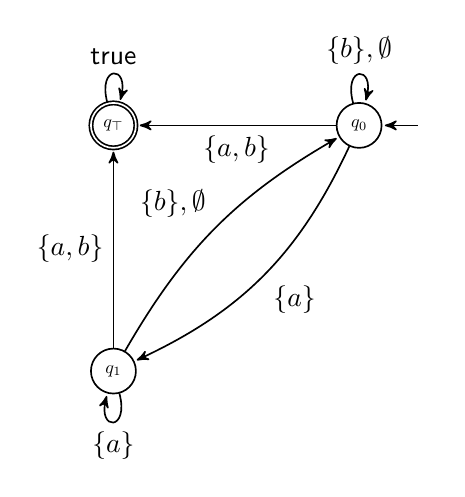
\begin{tikzpicture}[->,>=stealth',shorten >=1pt,auto,node distance=4.8cm,
                    semithick, initial text={}, initial where=right]
  \tikzstyle{every state}=[scale=0.65, every node/.style={scale=0.65}]

  \node[initial,state] (A)                {$\monstate_0$};
  \node[state, accepting]         (B) [left of  = A] {$\monstate_\top$};
  \node[state]         (D) [below of = B] {$\monstate_1$};

  \path (A) edge              node {$ \{a,b\}$} (B)
                 edge [loop above] node {$\{b\}, \emptyset$} (A)
                 edge      [bend left=20]     node   {$\{a\}$} (D)
        (B) edge [loop above] node {$\tru$} (B)
        (D) edge                 node {$\{a,b\}$} (B)
        (D) edge       [bend left=15]             node {$\{b\}, \emptyset$} (A)
        (D) edge [loop below] node {$\{a\}$} (D);

\end{tikzpicture}    
\caption{$\monitor_e^\varphi$ for $\varphi = \F (a \wedge b)$} 
\end{figure}
\label{fig:exltla&b}


Suppose monitors are at monitor state $\monstate_0$, and let $\state= \{a, b\} $. The following tables represent each monitor $M_i$'s initial \localreg~$\snap_i^\state$ and its verdict set $\verdict_i$ calculated based on only $\snap_i^\state$.



 \begin{tabular}{|c|c|c|c|}
   \multicolumn{1}{r}{} &  \multicolumn{2}{c}{ {$\snap_1^\state$}}\\
\hline
  & $M_1$ & $M_2$ & $M_3$\\
 \hline
   $a$ & $\tru$ & $\udef$ & $\udef$\\
   $b$ & $\udef$ & $\udef$ & $\udef$\\
\hline
  $\verdict_1$  &  \multicolumn{3}{c|}{\cellcolor{gray!25}$\{\monstate_1, \monstate_\top\}$}\\
\hline
  \end{tabular}  
\quad
 \begin{tabular}{|c|c|c|c|}
   \multicolumn{1}{r}{} &  \multicolumn{2}{c}{ {$\snap_2^\state$}}\\
\hline
  & $M_1$ & $M_2$ & $M_3$\\
 \hline
   $a$ & $\udef$ & $\udef$ & $\udef$\\
   $b$ & $\udef$ & $\tru$ & $\udef$\\
\hline
  $\verdict_2$  &  \multicolumn{3}{c|}{\cellcolor{gray!25}$\{\monstate_0, \monstate_\top\}$}\\
\hline
  \end{tabular}
\quad
 \begin{tabular}{|c|c|c|c|}
   \multicolumn{1}{r}{} &  \multicolumn{2}{c}{ {$\snap_3^\state$}}\\
\hline
  & $M_1$ & $M_2$ & $M_3$\\
 \hline
   $a$ & $\udef$ & $\udef$ & $\udef$\\
   $b$ & $\udef$ & $\udef$ & $\udef$\\
\hline
  $\verdict_3$  &  \multicolumn{3}{c|}{\cellcolor{gray!25}$\{\monstate_0, \monstate_1, \monstate_\top\}$}\\
\hline
  \end{tabular}   \\ \\




And by calculating the intersection of the verdict sets we obtain $\mathcal{I}^\monstate_0 = \monstate_\top$, which is the verdict that a centralized monitor that has full view of state $\state = \{a, b\}$ would compute. Note that a verdict form $\mathbb{B}_3$ can be emitted simply by applying the mapping function $\lambda_e$, i.e., by calculating $\lambda_e(v)$ where $v \in \intersection$, which in this example is $\lambda_e(\monstate_\top) = \top$.









\iffalse

\begin{tabular}{| c |c |c |c|}
\multicolumn{4}{c}{$M_1$} \\
\hline
&$M_1$&$M_2$ & $M_3$\\
\hline
$a$ & $true$ & $\natural$ & $\natural$ \\
$b$ & $\natural$ & $\natural$ & $\natural$\\
\hline
\end{tabular}  
\quad
\begin{tabular}{| c |c |c |c|}
\multicolumn{4}{c}{$M_1$} \\
\hline
&$M_1$&$M_2$ & $M_3$\\
\hline
$a$ & $\natural$ & $\natural$ & $\natural$ \\
$b$ & $\natural$ & $true$ & $\natural$\\
\hline
\end{tabular}  
\quad
\begin{tabular}{| c |c |c |c|}
\multicolumn{4}{c}{$M_1$} \\
\hline
&$M_1$&$M_2$ & $M_3$\\
\hline
$a$ & $\natural$ & $\natural$ & $\natural$ \\
$b$ & $\natural$ & $\natural$ & $\natural$\\
\hline
\end{tabular}  \\ \\








\subsection{The Overall Idea of The Automata-Based Algorithm}



We first introduce an algorithm that constructs an `\textit{\Exltl}'. The algorithm receives as input an \LTLtri monitor and solely based on the structure of the input monitor, it may add new monitor states to the original \LTLtri monitor. The \Exltl~ then is used in each local monitor $M_i$'s algorithm to consistently solve the decentralized asynchronous monitoring problem. As we will describe further, the intuition behind this algorithm is to monitor the system under inspection by taking the intersection of the sets of verdicts emitted by a set of distributed monitors. 


Let $\monitor^\varphi=\{\Sigma, Q, \delta, \monstate_0, F\}$ be the \LTLtri monitor for \LTL formula $\varphi$. Our goal is to construct an \Exltl~ $\monitor_e^\varphi =  \{ \alphabet, Q_e, \monstate_0, \delta_e , \lambda_e\}$ such that $|\intersection|=1$ at every monitor state $\monstate \in Q_e$.



\begin{definition}
 Let $\monitor^\varphi = \{ \alphabet, Q, \monstate_0, \delta , \lambda\}$ be the \LTLtri monitor for an \LTL formula $\varphi$. The \Exltl~ of $\varphi$ is the unique deterministic finite state machine $\monitor^\varphi_e = \{ \alphabet, Q_e, \monstate_0, \delta_e , \lambda_e\}$, where $Q_e$ is a set of states s.t. $Q \subseteq Q_e$, $q_0$ is the initial state, $\delta: Q_e \times \alphabet \rightarrow 2^Q_e $ is the transition function, and $\lambda_e : Q_e \rightarrow \mathbb{B}_3 $ is a mapping function, such that (1) for every non-empty finite trace $\alpha \in \alphabet^*$, we have $\lambda_e (\delta_e(q_0, \alpha)) = \lambda (\delta(q_0, \alpha))$, and (2) at every $\monstate \in Q_e$ we have $|\intersection| = 1$.
\end{definition}

Algorithm \ref{alg:extendedmonalg} constructs \Exltl. 




%\newcommand\mycommfont[1]{\tiny\ttfamily\textcolor{black}{#1}}
%\SetCommentSty{mycommfont}
%\usepackage[skins]{tcolorbox}
%\begin{tcolorbox}[blanker,width=(\linewidth-0.0cm)]


\begin{algorithm}[H]
\tiny
\KwIn{$\monitor^\varphi = \{ \alphabet, Q, \monstate_0, \delta , \lambda\}$}
\KwOut{$\monitor^\varphi_e = \{ \alphabet, Q_e, \monstate_0, \delta_e , \lambda_e\}$}           

\DontPrintSemicolon
$Q_e \leftarrow Q$ \\   \label{line:initExl}
\For {every $\monstate_i \in Q$}{
 \label{line:everystate}
 Obtain the set of outgoing transitions $T_i $ from monitor state $\monstate_i$   \\
 \label{line:outgoingtrans}
% \While {$T_i \neq \emptyset$}   {
   \For {every $t_j^i \in T_i$} {     
  \label{line:everytrans}
   \tcc*[r]{\it $t_j^i = \{s \in \alphabet ~|~  \delta(\monstate_i, s) = \monstate_j \}$}  
  
   \tcc*[r]{\it $N_j$ denotes the number of transitions from which $t_j^i$ is \indist, and $K_j$ denotes the number of transitions \indist~from $t_j^i$}
      $N_j \leftarrow 0 ~,~  K_j \leftarrow 0$      \\ 
    \label{line:initNK}
     \For {every $t_k^i \in T_i \backslash \{t_j^i\}$ } {     \label{line:indisting}
      \If{\indisting($t_j^i$, $t_k^i)$}{  \label{line:indistingfrom}
       $N_j \leftarrow N_j + 1$}
      \If{\indisting($t_k^i$, $t_j^i)$}{  \label{line:fromindisting}
       $K_j \leftarrow K_j + 1$}   \label{line:indistingend}
     }
     \If{$N_j > 0$}{ \label{line:split0}
      $\{t_{j1}^i, t_{j2}^i\}  \leftarrow \splitt(t_j^i, N_j, K_j, T_i) $  \label{line:split}
      
      $T_i \leftarrow \{ t_{j1}^i, t_{j2}^i\}  \cup T_i \backslash \{t_j^i\}$\\    \label{line:T-update}      
      $Q_e \leftarrow \{\monstate_{j1}, \monstate_{j2}\} \cup (Q_e \backslash   \{\monstate_j\})$ \\  \label{line:monstate-update}
      
      \If{$i \neq j$}{     \label{line:delta-update0}
         \For {every $t_k^i \in T_i$}{  \label{line:delta-oldtrans0}
           $\delta(\monstate_i, \state) = \monstate_k$ for every $\state \in t_k^i$   
         }
         $\delta(\monstate_{j1}, \state) \leftarrow \delta(\monstate_i, \state)$ for every $\state \in \alphabet$ \\  \label{line:delta-newtrans01}
         $\delta(\monstate_{j2}, \state) \leftarrow \delta(\monstate_i, \state)$ for every $\state \in \alphabet$       \label{line:delta-newtrans02}
      }
      \If{$i = j$}{   \label{line:delta-update1}  
          \For {every $t_k^i \in T_i$}{ \label{line:delta-oldtrans1}
           $\delta(\monstate_{j1}, \state) = \monstate_k$ for every $\state \in t_k^i$ 
         }
          $\delta(\monstate_{j2}, \state) \leftarrow \delta(\monstate_{j1}, \state)$ for every $\state \in \alphabet$         \label{line:delta-newtrans1}
      }
      
      $\lambda_e(\monstate_{j1})\leftarrow \lambda(\monstate_j)$ \\ \label{line:lambda-update0}
      $\lambda_e(\monstate_{j2})\leftarrow \lambda(\monstate_j)$ \\  \label{line:lambda-update1}
     }  \Else {
    
    
      $\delta_e(\monstate_i, s) \leftarrow \monstate_j$ for every $\state \in t_j^i$ \\  \label{line:delta-update2}
      $\lambda_e(\monstate_j)\leftarrow \lambda(\monstate_j)$ \\   \label{line:lambda-update2}
     }
   }   
% }      
} 

\caption{\Exltl~Construction}
\label{alg:extendedmonalg}
\end{algorithm}
%\end{tcolorbox}

%\begin{tcolorbox}[blanker,width=(\linewidth-0.1cm)]
\begin{algorithm}[H]
\DontPrintSemicolon
%\SetNoFillComment
  
\begin{algorithmic}
\tiny
\Function{\textit{\splitt}}{transition $t_j^i, N_j, K_j$, set of transitions $T_i$} 
\State $N_{j, min} \leftarrow N_j$   
\State $K_{j, min} \leftarrow K_j$    %\tcc*[r]{\it$N_j$ and $K_j$ are calculated in Algorithm \ref{alg:extendedmonalg}}

%\State $  \partition(t_j)$
\State \For {every $\{t_{j1}^{i,l}, t_{j2}^{i,l}\} \in \partition(t_j^i)$ }{
              
    $N_{jl} \leftarrow 0 ~,~ K_{jl} \leftarrow 0$ \
            
    \For {every $t_k^i \in  (\{t_{j2}^{i,l}\} \cup T_i \backslash \{t_j^i\})$ } {    
                  \If{\indisting($t_{j1}^{i,l}$, $t_k^i)$}{
                   $N_{jl} \leftarrow N_{jl}+1$}                     
                   \If{\indisting($t_k^i$, $t_{j1}^{i,l})$}{         
                    $K_{jl} \leftarrow K_{jl}+1$}
     }              
     \For {every $t_k^i \in  (\{t_{j1}^{i,l}\} \cup T_i \backslash \{t_j^i\})$ } {    
                  \If{\indisting($t_{j2}^{i,l}$, $t_k^i)$}{
                   $N_{jl} \leftarrow N_{jl}+1$}
                   \If{\indisting($t_k^i$, $t_{j2}^{i,l})$}{
                    $K_{jl} \leftarrow K_{jl}+1$}
                  
    } 
    \If {$(N_{jl}+K_{jl}) \leqslant (N_{j,min}+K_{j,min})$} {
       $l_{min} = l$
    }         
}          


  $  t_{j1}^i =  t_{j1}^{i,l_{min}},  t_{j2} ^i = t_{j2}^{i, l_{min}}$
  

\Return $\{t_{j1}^i, t_{j2}^i\}$
\EndFunction
\end{algorithmic}   

\begin{algorithmic}
\tiny
\Function{\textit{\partition}}{transition $t_j^i$}
  \State  compute all partitions $\{t_{j1}^{i,l} , t_{j2}^{i,l}\}$ of $t_j^i$ where $l \in [1 \cdots \frac{2^{| t_j^i|}-2}{2}]$, s.t.  
 \State for every pair $\{t_{j1}^{i,l} , t_{j2}^{i,l}\}$: 
  
  \begin{itemize}
  \item $t_{j1}^{i,l} \cup  t_{j2}^{i,l} = t_j^i$
  \item $t_{j1}^{i,l} \cap  t_{j2}^{i,l} = \emptyset$
  \end{itemize}
 
 \Return $\{\{t_{j1}^{i,1} , t_{j2}^{i,1}\}, \{t_{j1}^{i2} , t_{j2}^{i2}\}, \cdots , \{t_{j1}^{i, 2^\frac{2^{| t_j^i|}-2}{2}} , t_{j2}^{i, \frac{2^{| t_j^i|}-2}{2}} \}  \}$

\EndFunction
\end{algorithmic}

\caption{Functions \splitt~and \partition}
\end{algorithm}
%\end{tcolorbox} 
 
 
 \iffalse
 
\begin{algorithm}[H]   

\begin{algorithmic}
\tiny
\Function{\textit{\partition}}{transition $t_j^i$}
  \State  compute all partitions $\{t_{j1}^{i,l} , t_{j2}^{i,l}\}$ of $t_j^i$ where $l \in [1 \cdots \frac{2^{| t_j^i|}-2}{2}]$, s.t.  
 \State for every pair $\{t_{j1}^{i,l} , t_{j2}^{i,l}\}$: 
  
  \begin{itemize}
  \item $t_{j1}^{i,l} \cup  t_{j2}^{i,l} = t_j^i$
  \item $t_{j1}^{i,l} \cap  t_{j2}^{i,l} = \emptyset$
  \end{itemize}
 
 \Return $\{\{t_{j1}^{i,1} , t_{j2}^{i,1}\}, \{t_{j1}^{i2} , t_{j2}^{i2}\}, \cdots , \{t_{j1}^{i, 2^\frac{2^{| t_j^i|}-2}{2}} , t_{j2}^{i, \frac{2^{| t_j^i|}-2}{2}} \}  \}$

\EndFunction
\end{algorithmic}


 \begin{algorithmic}
 \tiny
\Function{\textit{\indisting}}{transition $t_1$, transition $t_2$}
  \State \If {there exists $\state \in t_2$ s.t. $\dep(\state, t_1)$}{
     \Return True} \Else {\Return False}
\EndFunction
\end{algorithmic}   

\begin{algorithmic}
\tiny
\Function{\textit{\dep}}{\event~$\state$, transition $t$}
  \State \If {$(\forall ap \in AP.~ \exists \state' \in t.~ (ap \in \state \Leftrightarrow ap \in \state' ))$}{
     \Return True} \Else {\Return False}
\EndFunction
\end{algorithmic}


\caption{Functions \partition, \indisting, and \dep}
\end{algorithm}  \ \

\fi















\newpage

\subsection*{Results}




\begin{lemma}
Let $f^r$ be the number of crashes at round $r$. The following holds:

`number of different local states obtained by monitors at round $r$' $\leq$ $min\{f^r+1, |AP|+1\}$
\end{lemma}


Let $M_r \subseteq M$ be the set of remaining monitors at the begining of round $r$, and $f_r$ be the number of crashes at round $r$.

\begin{lemma}
If $f_r<2$ or $|M_r| - f_r<2$ then at least one monitor knows the value of all propositions at the end of round r, i.e., $\exists M_i \in M_r$ such that  $\forall p_j \in AP$ we have $S^s_i(p_j) \neq \natural$. 
\end{lemma}


Let $V_i$ be the verdict set emitted by monitor $M_i$, and $I_r$ be the intersection of all verdict sets emitted by nonfaulty monitors at round $r$. 

\begin{lemma}
if $\exists M_i\in M_r$ such that  $\forall p_j\in AP$. $S^s_i(p_j) \neq \natural$, then we have $|I_r|=1$.
\end{lemma}


\begin{lemma}
If $nf<|AP|$ where $n\geq 1$, then there exists at least one monitor which knows the value of at least $n+1$ propositions.
\end{lemma}


\begin{lemma}
If $\forall r. (f_r\geq 2  \wedge  |M_r|-f_r\geq 2)$, then we have $|I_r|\neq1$ for every $r$ where $r < f +1$.
\end{lemma}

%\begin{lemma}
%In a synchronous system with up to $t$ crash failures solving consensus requires at least $t+1$ rounds (Ref3, Ref5).
%\end{lemma}

\begin{lemma}
Solving fault-tolerant distributed monitoring (FTDM) problem in a synchronous system with up to $t$ crash failures requires $f+1$ rounds.
\end{lemma}

\begin{lemma}
Increasing the number of rounds does not improve the minimum number of new monitor states required in the extended $LTL_3$ monitor.
\end{lemma}

\textit{Note:} The extended $LTL_3$ monitor for $\varphi$ is the monitor that we construct from the $LTL_3$ monitor of $\varphi$ to solve the synchronous fault-tolerant distributed monitoring in only one round of communication.


\begin{lemma}

If there are exactly $f$ faulty monitors, where $1 \leq f \leq t$, in every round then solving synchronous FTDM requires $f + 1$ rounds.

\end{lemma}



\subsection*{Proof}

Let $s$ be the state that is being monitored. Let $P = \{p_1 p_2 \cdots p_k\}$ be the set of all propositions and $FI = \{v^s_{p_1} v^s_{p_2} \cdots v^s_{p_k}\}$ be the set of values of all propositions at state $s$, we call it Full Information set. Each monitor's information about state $s$ is a subset of FI. It is easy to verify that, if there are $f_i$ crashes in round $r_i$, then the number of different subsets of FI that can be obtained as the monitor's information at the end of round $r_i$, is at most $f_i+1$. This occurs when no two crashed monitors send their information to the same uncrashed monitor. Clearly, the following conditions must also hold: \\ \\
$i)$the number of uncrashed monitors in round $r_i$ is at least $f_i+1$,   \\ 
$ii)$ $2^{|P|} \geq f_i+1$. 
\\ 

From the previous lemma we know that if $f_i = 1$ then the correct opinion is reached at round $r_i$. Therefore, the worst case happens if $f_i = 2$ for any $i$, i.e., there are exactly two crashes in each round. Suppose the two monitors that crash in the first round have different information about state $s$ (i.e., different subsets of FI) and they send their information to two differnet uncrashed monitors (whose information unioned by the received information is still not full information) and in the next round the same two monitors crash and send their information to two different uncrashed monitors and so on. Hence, it is easy to verify that in the worst case senario it is only after $f + 1$ number of rounds that at least one state obtains full information. 


%\subsubsection{\textbf{Upper bound on the number of rounds}}

In our setting the assumption is that the set of monitors satisfy the state coverage. Thus if a proposition is read by only one monitor, then this monitor is supposed to send its information to at least one nonfaulty monitor before crashing. A direct consequence of this assumption is the following lemma.

\begin{lemma}
If there is only one monitor crash in some round, then at least one monitor outputs the correct opinion at the same round. 
\end{lemma}

If only one monitor crashes in any round then, based on our assumption, it sends its information to at least one other monitor before crashing. Thus the monitor which receives the message from the crashed monitor has the value of all propositions (full information), and it outputs the correct opinion. 



\subsubsection{\textbf{Adding states to the FSM}}

In the previous section it was shown that in less than $f + 1$ rounds it is not guaranteed that at least one monitor has the full information about the current state and therefore outputs the correct opinion. So if the total number of crashes is large, the monitors have to communicate in many rounds. Hence, we take another approach by which we no longer require the monitors to communicate a mimimum number of rounds before they can output their final opinion. This can be done by adding new states to the original $LTL_3$ monitor. 

\subsubsection*{Examples}

\textbf{ $i)\mathbf{\Diamond (a \wedge b)}$}

\textbf{ $ii)\mathbf{\Diamond (a \vee b)}$}


Suppose each monitor reads only the value of one proposition (which is the worst case scenario), and it has to output its opinion only based on the value of that single proposition. Consider the monitor for $\Diamond (a \wedge b)$ above, suppose the current state is state $0$, and monitor 1($M_1$) only reads the value of $a$ and monitor 2($M_2$) only reads the value of $b$. Then if in the current state both $a$ and $b$ hold, then $M_1$ outputs $\{0,T\}$ since it does not know the value of $b$ and therefore from its point of view both states $0$ and $T$ are possible. Similarly, $M_2$ also outputs  $\{0,T\}$. Clearly, the correct opinion belongs to the intersection of all sets of opinions generated by monitors. Thus if the intersection consists of only one opinion, then it is the correct opinion. If the intersection includes more than one opinion, then we say that those opinions (equivalently states of monitor) are indistinguishable from each other in the viewpoint of the current state. 

\begin{claim}

Any two indistinguishable states can be turned into distinguishable states by adding new state(s) to the current monitor. 

\end{claim}

 For example in both above examples two indistinguishable states ($0$ and $T$) become distinguishable by adding state $1$ to the current monitors. 
 
 
 Based on this idea, we need to find an algorithm which receives as input a $LTL_3$ monitor and returns a new monitor with possibly equal or more number of states in which all states are distinguishable from the viewpoint of any state. In order to do so, we first build an algorithm that given a state and its transitions, detects all indistinguishable states from the viewpoint of that state. Then we write another algorithm  that starting from the initial state, sequentially generates and adds new states to the original monitor untill all states are distinguishable. 
 
 \subsubsection*{Algorithm to detect indistinguishable states}
 
 
 \begin{description}
 
 
 \item[1)] For every outgoing transition from the current state, list all propositions and their negations which appear on that transition. For example for $\Diamond (a \wedge b)$  at the initial state, the list of propositions/their negations on the outgoing transition to state $T$ is $SP_T = \{a, b, -a, -b\}$ and to state $0$ is $SP_0 = \{a, b\}$.
 
 \item[2)] For every pair of outgoing transitions verify whether $SP_i \subseteq SP_j$ or $SP_i \nsubseteq SP_j$. Then apply the following rules\\ 
 
 
$i)$ $SP_i \subseteq SP_j \Longrightarrow  j \in OP_i $  \\ \\
% $ii)$ $SP_i \subseteq SP_j \Longrightarrow  j \notin OP_i $  \\
 
 
 Where $SP_i$ and $SP_j$ are the sets of propositions/their negations for the outgoing transitions to states $i$ and $j$, respectively. And $OP_i$ (or $OP_j$)is the greatest intersection of the sets of opinions generated by all monitors, corresponding to the events that appear on the outgoing transition to state $i$ (or $j$). For example in the $LTL_3$ monitor for $\Diamond (a \wedge b)$,  we have $OP_0 = \{ 0 \}$ and $OP_T = \{0, T\}$.

We say state $i$ is indistinguishable from state $j$, if $ j \in OP_i $.
 
 
 
 \end{description}
 
 

\fi
          
        % \setcounter{figure}{0}
       % \setcounter{equation}{0}
       % \setcounter{table}{0}





% \chapter{Alternation Number for \LTL Formula}


\section{The Alternation Number: Previous Work}

\section{Calculating the Alternation Number for \LTL Formula}
\label{sec:AN}


\subsection{Alternation Number for $\varphi_1 \, \cup \, \varphi_2$}

\begin{definition}

 Let  $\varphi_1$ and $\varphi_2$ be $LTL$ formulas and $\alpha = 
\alpha_0\alpha_1\cdots \alpha_{n}$ be a finite word.\\

$   [ \alpha \models_F \varphi_1 \, \cup \, \varphi_2] =  \left\{ \begin{array}{rcl} \top & \mbox{if}
         & \exists k \in [0,n] \, : \, [\alpha_k \models_F \varphi_2] = \top\, \wedge \, \\& \mbox{} & \mbox{} \forall l \in [0,k] \, : \, [\alpha_l \models_F \varphi_1] = \top  \\ \bot  & \mbox{otherwise} \end{array}\right. $ 

\end{definition}
~~~

%\begin{theorem}


%$  \left. 
%\begin{cases}
%\text{if} ~ AN(\varphi_2) = 0 & ~~~~  AN(\varphi_1 \, \cup \, \varphi_2) = 1  \\ 
%\text{if} ~ AN(\varphi_2) \geq 1 & ~~~~  AN(\varphi_1 \, \cup \, \varphi_2) \leq \infty \\
%\text{if} ~  AN(\varphi_2) \geq 1 ~ \text{and} ~ \varphi_2  ~ \text{is a co-safety property} & ~~~~ AN(\varphi_1 \, \cup \, varphi_2) = AN(\varphi_2)\\
%\text{if} ~  AN(\varphi_2) \geq 1 ~ \text{and} ~ \varphi_2  ~ \text{is a safety property} & ~~~~ AN(\varphi_1 \, \cup \, \varphi_2) \leq \infty\\
%\end{cases}\right. $

%\end{theorem}


\begin{lemma}

If $\varphi$ is a safety formula, then its maximum alternating sequence ends with an illegal state. 

\end{lemma}

\subparagraph{Proof}
The proof is by contradiction. Let $\alpha = s_0s_1s_2 \cdots s_{n-1} s_n $ be the maximum alternating sequence for safety property $\varphi$. Suppose it ends with a legal state, i.e., $[s_0s_1s_2 \cdots s_{n-1} s_n \models_F \varphi] = \top$. Then it follows that $[s_0s_1s_2 \cdots s_{n-1} \models_F \varphi] = \bot$. We can employ the infinite trace $\alpha = s_0 s_1 s_2 \cdots s_{n-1} s_{n-1} s_{n-1} \cdots$ as a counter example which does not satisfy the safety formula $\varphi$, however, there is no bad prefix for it; since state $s_n$ can be added to any prefix of $\alpha$ to turn it to a legal trace.  

\begin{lemma}

If $\varphi$ is a co-safety formula, then its maximum alternating sequence ends with a legal state. 

\end{lemma}

\subparagraph{Proof}
The proof is similar to lemma 1. Let $\alpha = s_0s_1s_2 \cdots s_{n-1} s_n $ be the maximum alternating sequence for co-safety property $\varphi$. Suppose it ends with an illegal state, i.e., $[s_0s_1s_2 \cdots s_{n-1} s_n \models_F \varphi] = \bot$. Then it follows that $[s_0s_1s_2 \cdots s_{n-1} s_n \models_F \varphi] = \top$. \\
We can employ the infinite trace $\alpha = s_0 s_1 s_2 \cdots s_{n-1} s_{n-1} s_{n-1} \cdots$ as a counter example which satisfies the co-safety formula $\varphi$, however, there is no good prefix for it; since state $s_n$ can be added to any prefix of $\alpha$ to turn it to an illegal trace.  \\




\begin{theorem}

If $\varphi$ is a safety or co-safety formula, then $AN(\varphi) \leq 1$

\end{theorem} 

\subparagraph{Proof}

We prove this theorem by contradiction. First, suppose $\varphi$ is a safety formula and its alternation number is greater than 1, e.g., $AN(\varphi) = 2$, and let $\alpha = s_0 s_1 s_2$ represent the maximum alternating trace for $\varphi$.  Since $AN(\varphi) = 2$ and considering lemma 1, there is only one possible scenario for alternation of $\varphi$ over $\alpha$ which is as follows,\\ 


\begin{center}
$\left.
\begin{cases}
[s_0 \models_F \varphi] = \bot_p\\
[s_0 s_1 \models_F \varphi] = \top_p\\
[s_0 s_1 s_2 \models_F \varphi] = \bot \\
\end{cases}
\right.
$
\end{center}

We observe that an infinite trace can be defined as $ \alpha = s_0 s_0 s_0 \cdots $ which does not satisfy the safety formula $\varphi$, however, there is no bad prefix for it. Because any prefix of $\alpha$ can be extended to state $s_1$ where $\varphi$ is satisfied. This contradicts with our assumption of $\varphi$ being a safety property and the proof is complete. 

Now suppose $\varphi$ is co-safety formula $AN(\varphi) \geq 1$, i.e., $AN(\varphi) = 2$. Let $\alpha = s_0 s_1 s_2$ be the maximum alternating trace for $\varphi$. Based on lemma 2, the only possible alternation of $\varphi$ over $\alpha$ is as follows,

\begin{center}
$\left.
\begin{cases}
[s_0 \models_F \varphi] = \top_p\\
[s_0 s_1 \models_F \varphi] = \bot_p\\
[s_0 s_1 s_2 \models_F \varphi] = \top \\
\end{cases}
\right.
$
\end{center}

Then, an infinite trace $ \alpha = s_0 s_0 s_0 \cdots $ can be defined, which satisfies co-safety formula $\varphi$ but it does not have a good prefix, since any prefix of $\alpha$ can be extended to state $s_1$ which satisfies $\varphi$. This is a contradiction as we assumed $\varphi$ is a co-safety formula. Thus, the proof is complete.


~\\


\begin{theorem}

$ 
% AN(\varphi_1 \, \cup \, \varphi_2) =
 \left. 
\begin{cases} 
 \text{if} ~ AN(\varphi_2) = 0 ~  \text{or} ~ \varphi_2 ~ \text{is a co-safety property,} & AN(\varphi_1 \, \cup \, \varphi_2) \leq 1. \\ 
 \text{Otherwise,} \\
\text{if} ~ \varphi_1~  \text{and}~ \varphi_2 ~ \text{do not share variables} \\
 \text{and} ~ \varphi_1 \neq \text{False,}  & AN(\varphi_1 \, \cup \, \varphi_2) = \infty~ \text{or}~ AN(\varphi_2)\\
\end{cases}\right. $  \\  \\
  
%\textbf{Note:} $(\leq)$ becomes $(=)$ if $\varphi_1$ and $\varphi_2$ do not share variables.

\end{theorem}



\subparagraph{Proof}

%\subsection*{}

We prove the first statement of the theorem by contradiction. Suppose $AN(\varphi_2) = 0$ and $AN(\varphi_1 \, \cup \, \varphi_2)$ can be greater than 1, e.g., $AN(\varphi_1 \, \cup \, \varphi_2) = 2$. \\ 
Without loss of generality, let $\alpha = s_0 s_1 s_2$ represent the finite trace over which we verify the correctness of the formula. Since $AN(\varphi_1 \, \cup \, \varphi_2) = 2$, there can be two possible scenarios.\\
\textit{Note} : Throughout this proof we label a state $s_i$ by $\top$ if the formula is satisfied by the finite trace starting at $s_i$ and we label it by $\bot$ otherwise. 

\subsection*{}

\textit{Scenario 1.} \\

First scenario is as follows, 
~~~
 \begin{center}
 $
  \left.
  \begin{cases}
    [s_0 \, \models_F \, \varphi_1 \, \cup \, \varphi_2] = \top \\
    [s_0 s_1 \, \models_F \, \varphi_1 \, \cup \, \varphi_2] = \bot \\
     [s_0 s_1 s_2\, \models_F \, \varphi_1 \, \cup \, \varphi_2] = \top \\
  \end{cases}
  \right.
$
\end{center}

~~
%\[
 %    \left\{\begin{array}{lr}
 %       x(n), & \text{for } 0\leq n\leq 1\\
  %      x(n-1), & \text{for } 0\leq n\leq 1\\
   %     x(n-1), & \text{for } 0\leq n\leq 1
   %     \end{array}\right.
 % \]
  
$s_0$ holds only if $[s_0 \, \models_F \, \varphi_2] = \top$ (in general, any finite trace may satisfy $\varphi_1 \, \cup \, \varphi_2$ only if it satisfies $\varphi_2$. This is directly implied by Definition 1).  Also, $[s_0 s_1 \, \models_F \,  \varphi_1 \, \cup \, \varphi_2] = \bot$ holds only if $[s_0 s_1 \, \models_F \, \varphi_2] = \bot$. Hence, we have  
~~~
 \begin{center}
$
  \left.
  \begin{cases}
    [s_0 \, \models_F \, \varphi_2] = \top \\
    [s_0 s_1 \, \models_F \, \varphi_2] = \bot \\
  \end{cases}
  \right. 
\Longrightarrow     ~~~   AN(\varphi_2) > 0
$
\end{center}
  
  Which contradicts with our assumption $AN(\varphi_2) = 0$. This means that if the alternation number of $\varphi_2$ is zero, the valuation of $\varphi_1 \, \cup \, \varphi_2$ can never alter from True to False over any finite trace. 


\subsection*{}

\textit{Scenario 2}

The second scenario is as follows,
~~~
 \begin{center}
 
$  \left.
  \begin{cases}
    [s_0 \, \models_F \, \varphi_1 \, \cup \, \varphi_2] = \bot \\
    [s_0 s_1 \, \models_F \, \varphi_1 \, \cup \, \varphi_2] = \top \\
    [s_0 s_1 s_2\, \models_F \, \varphi_1 \, \cup \, \varphi_2] = \bot \\
  \end{cases}
  \right.
  $
\end{center}
~~~ \\
 $[s_0 \, \models_F \, \varphi_1 \, \cup \, \varphi_2] = \bot$ leads to $ [s_0 \, \models_F \, \varphi_2] = \bot $. 
 $[s_0 s_1 \, \models_F \, \varphi_1 \, \cup \, \varphi_2] = \top$ can hold only if $ [s_1 \, \models_F \, \varphi_2] = \top $ and $ [s_0 \, \models_F \, \varphi_1] = \top$. 
Also, from $ [s_0 s_1 \, \models_F \, \varphi_1 \, \cup \, \varphi_2] = \top$ and $ [s_0 s_1 s_2\, \models_F \, \varphi_1 \, \cup \, \varphi_2] = \bot $ we can conclude that $[s_1 s_2\, \models_F \, \varphi_2] = \bot$. Because if $[s_1 s_2\, \models_F \, \varphi_2] = \top$, then $s_0s_1s_2$ cannot violate $\varphi_1 \, \cup \, \varphi_2$, since $\varphi_2$ is True at $s_1$ and $\varphi_1$ holds at $s_0$. Thus, we have

 \begin{center}
$
  \left.
  \begin{cases}
    [s_1 \, \models_F \, \varphi_2] = \top \\
    [s_1 s_2 \, \models_F \, \varphi_2] = \bot \\
  \end{cases}
  \right. 
\Longrightarrow     ~~~   AN(\varphi_2) > 0
$
\end{center}


Which again contradicts with our assumption $AN(\varphi_2) = 0$. Now the proof for the first statement of Theorem 1 is complete. \\ \\ 


The second statement claims that if $\varphi_2$ is a co-safety property, then the alternation number for $ \varphi_1 \, \cup \, \varphi_2$ is equal to 1. If $\varphi_2$ is a co-safety property then based on lemma 2 and theorem 1, its legality can alternate only once and only from illegal to legal state over any finite/infinite trace. 
Now let us verify the maximum number of times that the legality of $ \varphi_1 \, \cup \, \varphi_2$ may alternate over an infinite trace. As mentioned before, the maximum alternation for $ \varphi_1 \, \cup \, \varphi_2$ can be obtained over a trace where $\varphi_1$ holds in all states and the valuation of $ \varphi_1 \, \cup \, \varphi_2$ alternates based on the alternation of $\varphi_2$ only. In this case, since $\varphi_2$ is a co-safety property, its valuation can only change from False to True and once it becomes True it can never become False over any infinite trace. Thus, the valuation of $ \varphi_1 \, \cup \, \varphi_2$ can also alternate once from False to True. 

Our assertion is, that if $\varphi_2$ is not co-safety and its alternation number is greater than zero, then the alternation number for $ \varphi_1 \, \cup \, \varphi_2$ could be infinity. Because in this case, there most be at least one alternation from True to False for $\varphi_2$ over its maximum alternating trace. Thus, there are states $s_0$ and $s_1$ such that $\varphi_2$ holds in $s_0$ and it does not hold in $s_1$.  It is straightforward to verify that $ \varphi_1 \, \cup \, \varphi_2$ may alternate infinitely many times over the following infinite trace:

\begin{center}
$\alpha = s_0s_1s_0s_1s_0s_1 \cdots$
\end{center}

And the alternation is as follows,

 \begin{center}
$
  \left.
  \begin{cases}
    [s_0 \, \models_F \, \varphi_1 \, \cup \, \varphi_2] = \top \\
    [s_0 s_1 \, \models_F \, \varphi_1 \, \cup \, \varphi_2] = \bot \\
    [s_0 s_1 s_0 \, \models_F \, \varphi_1 \, \cup \, \varphi_2] = \top \\
    [s_0 s_1 s_0 s_1 \, \models_F \, \varphi_1 \, \cup \, \varphi_2] = \bot \\
    \vdots
  \end{cases}
  \right. 
$
\end{center}

The first two rows can be directly obtained from the assumptions $[s_0 \, \models_F \, \varphi_2] = \top$ and $[s_0s_1 \, 
\models_F \, \varphi_2] = \bot$. 

$[s_0 s_1 s_0 \, \models_F \, \varphi_1 \, \cup \, \varphi_2] = \top$ holds, because $\varphi_2$ is True in the last state, $s_0$, and $\varphi_1$ holds over the preceding states. 

(I need to edit this part) Let us verify $[s_0 s_1 s_0 s_1 \, \models_F \, \varphi_1 \, \cup \, \varphi_2] = \bot$. Here we need to evaluate three possible scenarios. \\
Scenario 1: $[s_0 s_1 s_0 \, \models_F \, \varphi_2] = \top_p$, in this case the alternation number for $\varphi_2$ is infinity over the infinite trace $\alpha = s_0s_1s_0s_1s_0s_1 \cdots$. Hence, the alternation number for $ \varphi_1 \, \cup \, \varphi_2$  is also infinity. \\ Scenario 2: $[s_0 s_1 s_0 \, \models_F \, \varphi_2] = \bot$, in this case the alternation number for $ \varphi_1 \, \cup \, \varphi_2$ is again infinity. \\ Scenario 3: $[s_0 s_1 s_0 \, \models_F \, \varphi_2] = \top$, in this case the alternation number for $ \varphi_1 \, \cup \, \varphi_2$ is 2. \\ Scenario 4: $[s_0 s_1 s_0 \, \models_F \, \varphi_2] = \bot_p$ and $[s_0 s_1 s_0 s_1 \, \models_F \, \varphi_2] = \top$, in this case the alternation number for $ \varphi_1 \, \cup \, \varphi_2$ is 2.











\subsection{Alternation Number for $\varphi_1 \, \wedge \, \varphi_2$  and $\varphi_1 \, \vee \, \varphi_2$}



\begin{theorem}

$
% AN(\varphi_1 \, \cup \, \varphi_2) =
 \left. 
\begin{cases} 
 AN(\varphi_1 \, \wedge \, \varphi_2) \leq AN(\varphi_1) + AN(\varphi_2) \\ 
 AN(\varphi_1 \, \vee \, \varphi_2) \leq AN(\varphi_1) + AN(\varphi_2)\\
\end{cases}\right. $  \\  \\

\end{theorem}

\subparagraph{Proof}

The maximum alternation number for $\varphi_1 \, \wedge \, \varphi_2$  can be obtained on a finite trace where one of the formulas, e.g., $\varphi_1$, may stay True while the other formula, e.g, $\varphi_2$, alternates $AN(\varphi_2)$ times. Then $\varphi_2$ can stay True while $\varphi_1$ alternates $AN(\varphi_1)$ times. Hence, the maximum alternation number for $\varphi_1 \, \wedge \, \varphi_2$ is equal to $AN(\varphi_1) + AN(\varphi_2)$. 
Since $\varphi_1 \, \vee \, \varphi_2$ is logically equivalent to $ - ( -\varphi_1 \, \wedge \, -\varphi_2)$, we can use the similar argue as for $\varphi_1 \, \wedge \, \varphi_2$, and hence, the upper bound for $AN(\varphi_1 \, \vee \, \varphi_2) $ is, too, $AN(\varphi_1) + AN(\varphi_2)$.





          
       % \setcounter{figure}{0}
       % \setcounter{equation}{0}
       % \setcounter{table}{0}

 \chapter{Conclusion}
\label{chap:Conclusion}

\section{Summary}


In this thesis, we studied synchronous and asynchronous runtime verification of 
distributed systems and presented distributed monitoring algorithms 
for this purpose, which allow three-valued LTL monitoring. In particular,

\begin{itemize}

\item we proposed a synchronous monitoring algorithm that copes with $f$ crash 
failures in a distributed setting. The algorithm solves the synchronous 
monitoring problem in $f+1$ rounds of communication, where at each round each 
local monitor broadcasts a message, receives messages from other monitors, and 
performs local computation based on the received messages and computes a message 
to be sent in the subsequent round. We proposed an automata-based algorithm 
where each local monitor's message is a set of monitor states that are reachable 
from the current monitor state (according to the input automaton) by the set of 
possible global states from viewpoint of that local monitor. Therefore our 
algorithm reduces the message size overhead from $|\AP|$ to $\log(m_\monstate)$ 
where $m_\monstate$ is the number of outgoing transitions from the current 
monitor state $\monstate$. We showed that the input automaton (that is employed 
in each monitor's algorithm) must satisfy the following condition:
$$\forall \monstate \in Q.~ |\intersection| = 1$$ where $Q$ is the set of all 
monitor states in the input automaton, and $\intersection$ denotes the 
intersection of all verdict sets emitted by local monitors. Therefore we 
introduced an algorithm to construct an \Exltl~that satisfies the aforementioned 
condition.

\item We proposed an algorithm for distributed crash-resilient asynchronous RV that consistently monitors the system under inspection without any communication between monitors. Each local monitor emits a verdict set solely based on its own partial observation, and the intersection of the verdict sets will be the same as the verdict computed by a centralized monitor that has full view of the system. 

\end{itemize}


\section{Future Work}

Some open problems for further research are as follows:

\begin{itemize}

\item In our framework the fault model was crash failure, i.e., the monitors can only fail by crashing. From a more practical perspective, it would be interesting to address more severe, e.g., Byzantine failures.

\item In the asynchronous monitoring, although we assumed the monitors are 
asynchronous wait-free processes, however, it was supposed that the global state 
of the system changes synchronously, i.e., all monitors observe the same 
global state. We can relax the timing model so that monitors observe, 
communicate, and emit verdicts between any two global states. 

\item Our results in the decentralized asynchronous monitoring can 
theoretically be transformed to more practical refinements such as message 
passing frameworks.

\item It would of course be interesting to extend our results to the case where 
the input to the monitors is a sequence of global states and each monitor 
produces a sequence of verdict sets, one per each global state. 

\end{itemize}
          
        % \setcounter{figure}{0}
       % \setcounter{equation}{0}
       % \setcounter{table}{0}


% \appendix

\chapter{Your Appendix}

Your appendix goes here.
               % you can include your appendix if you have any!

%\bibliographystyle{abbrv}

\bibliographystyle{natbib}
\bibliography{bibliography.bib}        % your list of references

\label{NumDocumentPages}

\end{document}